\documentclass[11pt,a4paper,hyphens]{report}
\usepackage{color}
\usepackage{caption}
\usepackage{translit}
\usepackage{amsmath}
% dasselbe Template wie Thesis mit nur leichten Anpassungen
% Nehmen Sie das Thesis-Template für die Thesis!
% Lesen Sie Hinweise zum Umgang mit LaTeX und zum Schreiben
% von Berichten im Thesis-Template nach
% => Moodle => PraxissemesterThesis => LaTeXThesis.zip
%    https://moodle.hs-mannheim.de/course/view.php?id=2500


% Für doppelseitigen Ausdruck (nur bei > 60 Seiten sinnvoll)
% \usepackage{ifthen}
% \setboolean{@twoside}{true}
% \setboolean{@openright}{true} 

% pakete
\usepackage{ifthen}

% Deutsch
\usepackage[german]{babel} % deutsch und deutsche Rechtschreibung
\usepackage[backend=biber, style=numeric, sorting=none]{biblatex} % Literaturverzeichnis (sortiert nach Reihenfolge des Auftretens)
\addbibresource{praksem.bib}
\usepackage[utf8]{inputenc} % Unicode Text
\usepackage[T1]{fontenc} % Umlaute und deutsches Trennen
\usepackage{textcomp} % Euro
% statt immer Ab\-schluss\-ar\-beit zu schreiben
% einfach hier sammeln mit -. 
\hyphenation{Ab-schluss-ar-beit}
% Vorsicht bei Umlauten und Bindestrichen
\hyphenation{Ver-st\"ar-ker-aus-gang}
 % eigene Hyphenations, die für das Dokument gelten
\usepackage{amssymb} % Symbole
\usepackage{emptypage} % Wirklich leer bei leeren Seiten

%% Fonts, je ein kompletter Satz an Optionen

% Times New Roman, gewohnter Font, ok tt und serifenlos
%\usepackage{mathptmx} 
%\usepackage[scaled=.95]{helvet}
%\usepackage{courier}

% Palatino mit guten Fonts für tt und serifenlos
\usepackage{mathpazo} % Palatino, mal was anderes
\usepackage[scaled=.95]{helvet}
\usepackage{courier}

% New Century Schoolbook sieht auch nett aus (macht auch tt und serifenlos)
%\usepackage{newcent}

% Oder default serifenlos mit Helvetica 
% ich kann es nicht mehr sehen ...
%\renewcommand{\familydefault}{\sfdefault}

% ein bisschen eine bessere Verteilung der Buchstaben...
\usepackage{microtype}

% Bilder und Listings
\usepackage{graphicx} % wir wollen Bilder einfügen
\usepackage{subfig} % Teilbilder
\usepackage{wrapfig} % vielleicht doch besser vermeiden
\usepackage{listings} % schöne Quellcode-Listings
% ein paar Einstellungen für akzeptable Listings
\lstset{basicstyle=\ttfamily, columns=[l]flexible, mathescape=true, showstringspaces=false, numbers=left, numberstyle=\tiny}
\lstset{language=python} % und nur schöne Programmiersprachen ;-)
% und eine eigene Umgebung für Listings
\usepackage{float}
\newfloat{listing}{htbp}{scl}[chapter]
\floatname{listing}{Listing}

% Seitenlayout
\newcommand{\seitenseitenabstand}{22mm} % 30mm
\usepackage[paper=a4paper,left=\seitenseitenabstand,right=\seitenseitenabstand,height=23cm]{geometry}
\usepackage{setspace}
% \linespread{1.15}
\linespread{1.1}
\setlength{\parskip}{0.5em}
\setlength{\parindent}{0em} % im Deutschen Einrückung nicht üblich, leider

% Seitenmarkierungen 
\newcommand{\phv}{\fontfamily{phv}\fontseries{m}\fontsize{9}{11}\selectfont}
\usepackage{fancyhdr} % Schickere Header und Footer
\pagestyle{fancy}
\renewcommand{\chaptermark}[1]{\markboth{#1}{}}
%\fancyhead[L]{\phv \leftmark}
\fancyhead[RH,LO]{\phv \nouppercase{\leftmark}}
\fancyhead[LH,RO]{\phv \thepage}
% Unten besser auf alles Verzichten
%\fancyfoot[L]{\textsf{\small \kurztitel}}
\fancyfoot[C]{\ } % keine Seitenzahl unten
%\fancyfoot[R]{\textsf{\small Technische Informatik}}

% Include subsubsections in the Table of Contents
% -1 for part
%  0 for chapter (only in report and book document classes)
%  1 for section
%  2 for subsection
%  3 for subsubsection
%  4 for paragraph
%  5 for subparagraph
\setcounter{tocdepth}{3}

% Theorem-Umgebungen
\newtheorem{definition}{Definition}[chapter]
\newtheorem{satz}{Satz}[chapter]
\newtheorem{lemma}[satz]{Lemma} % gleicher Zähler wie Satz
\newtheorem{theorem}{Theorem}[chapter]
\newenvironment{beweis}[1][Beweis]{\begin{trivlist}
                                       \item[\hskip \labelsep {\textit{#1 }}]}{
\end{trivlist}}
\newcommand{\qed}{\hfill \ensuremath{\square}}

%% Quellen
% Eine Alternative wäre Quellen in Literatur und Online-Quellen
% zu teilen
% \usepackage{bibtopic} 

% Hochschule Logo, noch nicht perfekt
\usepackage{hsmalogo}

% Spezialpakete
\usepackage{epigraph}
\setlength{\epigraphrule}{0pt} % kein Trennstrich

% damit wir nicht so viel tippen müssen, nur für Demo 
% \usepackage{blindtext}

% ifthen für sperrvermerk
\newif\ifsperrvermerk

% klickbare links im inhaltsverzeichnis
\usepackage{hyperref}
\hypersetup{
    colorlinks,
    citecolor=black,
    filecolor=black,
    linkcolor=black,
    urlcolor=black
}

% text shortcut variablen
\newcommand{{\metaeffekt}}{\{met\ae ffekt\}}
\newcommand{\bitkom}{bitkom}
\newcommand{\aeclientZEZESE}{Thales}
\newcommand{\headerand}{und\ }
% weekdays
\newcommand{\weekdayMondayLong}{Mo} % Mo, Montag
\newcommand{\weekdayTuesdayLong}{Di} % Di, Dienstag
\newcommand{\weekdayWednesdayLong}{Mi} % Mi, Mittwoch
\newcommand{\weekdayThursdayLong}{Do} % Do, Donnerstag
\newcommand{\weekdayFridayLong}{Fr} % Fr, Freitag
\newcommand{\weekdaySaturdayLong}{Sa} % Sa, Samstag
\newcommand{\weekdaySundayLong}{So} % So, Sonntag
\newcommand{\weekdayMondayShort}{Mo}
\newcommand{\weekdayTuesdayShort}{Di}
\newcommand{\weekdayWednesdayShort}{Mi}
\newcommand{\weekdayThursdayShort}{Do}
\newcommand{\weekdayFridayShort}{Fr}
\newcommand{\weekdaySaturdayShort}{Sa}
\newcommand{\weekdaySundayShort}{So}

% custom commands
\newcommand{\lweekdaymarginpar}[1]{%
    \marginpar{\raisebox{-1.6em}{\underline{#1}}}
}
\newcommand{\sweekdaymarginpar}[1]{%
    \marginpar{\raisebox{-1.92em}{\underline{#1}}}
}
\newcommand{\qt}[1]{„#1“}

\definecolor{codegray}{gray}{0.9}
\newcommand{\code}[1]{\colorbox{codegray}{\texttt{\detokenize{#1}}}}
\newcommand{\codendt}[1]{\colorbox{codegray}{\texttt{#1}}}

% custom environments
\newenvironment{smitemize}
{ \begin{itemize}
      \setlength{\itemsep}{0em}
      \setlength{\topsep}{0em}
      \setlength{\partopsep}{0em} }
      {
\end{itemize} }

% code listings
\input{latex-listings-powershell/src/latex-listings-powershell}
\definecolor{lst-gray}{rgb}{0.98,0.98,0.98}
\definecolor{lst-blue}{RGB}{40,0.0,255}
\definecolor{lst-green}{RGB}{65,128,95}
\definecolor{lst-red}{RGB}{200,0,85}
\lstset{
    commentstyle=\color{lst-green},
    basicstyle=\small\ttfamily,
    backgroundcolor=\color{lst-gray},
    breaklines=true,
    captionpos=b,
    columns=fixed,
    extendedchars=true,
    frame=single,
    framesep=2pt,
    keepspaces=true,
    keywordstyle=\color{lst-blue},
    language={PowerShell},
    numbers=left,
    numberstyle=\small\ttfamily,
    showstringspaces=false,
    stringstyle=\color{lst-red},
    tabsize=2,
}
 % alle Pakete und Einstellungen

% Hier anpassen 
\newcommand{\autor}{Yan Wittmann}
\newcommand{\matrikelnummer}{2121578}
\newcommand{\fachsemester}{5IB} % im wie vielten Semester waren Sie?
%\newcommand{\studiengang}{Medizintechnik}
%\newcommand{\studiengang}{Technische Informatik}
\newcommand{\studiengang}{Informationstechnik}
\newcommand{\firma}{\metaeffekt\ GmbH}
\newcommand{\standort}{Heidelberg}
\newcommand{\abteilung}{Automated Vulnerability Monitoring}
\newcommand{\betreuer}{Karsten Klein}
\newcommand{\pbeginn}{01.09.2023}
\newcommand{\pende}{29.02.2024}
\newcommand{\tage}{124} % arbeitstagerechner verwenden!
\newcommand{\titel}{Bericht zum praktischen Studiensemester}
\newcommand{\kurztitel}{Praxisbericht}
% \sperrvermerktrue % Kommentar am Anfang der Zeile löschen für Sperrvermerk

% entweder der vollständige oder der gekürzte Bericht
\newif\ifshortenedReport
\shortenedReporttrue

% Wenn jemand unbedingt ein Glossar will, die nächsten drei Zeilen...
%\usepackage{glossaries} % oder schlimmer mit [toc], damit es im TOC auftaucht
%\makeglossaries
%\newglossaryentry{Computer}{name=Computer,
    description={Eine programmierbare Maschine, die Eingaben erhält, Daten speichert und manipuliert
    und Ausgaben in einem sinnvollem Format ausgibt. (Und wer so was in ein Glossar eines Berichts
    für einen technischen Studiengang schreibt hat es nicht verstanden)}}
\newglossaryentry{naiv}{name=na\"{\i}ve,
description={Ein franzöisches Lehnswort (Adjektiv, Form von naïf)
Erweckt den Eindruch oder hat mangelnde Erfahrung, mangelndes Verständnis oder mangelnde Skills}}
\newglossaryentry{Linux}{name=Linux,
description={Generischer Ausdruck für eine Familie von Unix-artigen Betriebssystemen die den
Linux-Kernel verwenden},
plural=Linuces}
\newacronym[longplural={Frames per Second}]{fpsLabel}{FPS}{Frame per Second}
\newacronym{acme}{ACME}{A Company Making Everything}
\newglossaryentry{Praktisches Studiensemester}{name=Praktisches Studiensemester,
description={Im Rahmen des Ingenieursstudiums ein Semester in der betrieblichen Praxis
zur Ergänzung und Vertiefung des Studienwissens durch selbstständige ingenieurnahe Tätigkeit
betreut durch einen Ingenieur des Betriebes}}
 % In dieser Datei die Einträge definieren
% und noch ganz unten printglossaries auskommentieren
% Damit jetzt ein Glossar gezeigt wird noch \gls{label} verwenden

\begin{document}
    \begin{titlepage}
    \hsmalogo[1] \hfill
    \parbox[b]{60mm}{
        Fakultät Informationstechnik\\
        Studiengang \studiengang}
    \begin{center}
        \rule{1\textwidth}{1pt}\\[-3mm]
        \parbox[t][64mm]{110mm}{% 11 cm für Breite 13, ca. 7 für Höhe 6
            \Large{\ } \\[8mm]
            Bericht zum praktischen Studiensemester \\[4mm]
            \begin{tabular}{rl}
                \large{Vorgelegt von} & \large{\autor} \\[2mm]
                \large{Studiengang}   & \large{\studiengang} \\[2mm]
                \large{Firma}         & \large{\firma} \\[2mm]
            \end{tabular}
        }
        \rule{\textwidth}{1pt}
        \vfill
    \end{center}

    \vspace{2em}
    \begin{tabular}{ll}
        Name               & \autor                   \\
        Matrikelnummer     & \matrikelnummer          \\
        Studiengang        & \studiengang             \\
        Fachsemester       & \fachsemester \\[8mm]

        Praktikumszeitraum & \pbeginn\ \ bis \ \pende \\
        Präsenztage        & \tage \\[8mm]

        Firma              & \firma                   \\
        Standort           & \standort                \\
        Abteilung          & \abteilung               \\
        Betreuer           & \betreuer                \\
    \end{tabular}

    \vspace{8em}
    \noindent\begin{tabular}{p{0.48\textwidth}p{0.48\textwidth}}
                 \rule{0.46\textwidth}{0.5pt} & \rule{0.46\textwidth}{0.5pt} \\
                 Datum, \betreuer             & Firmenstempel
    \end{tabular}
    \vfill
\end{titlepage}
\cleardoublepage


% Erklärung gemäß der Prüfungsordnung
\thispagestyle{empty}
\subsection*{Selbstständigkeitserklärung}

Ich versichere, dass ich diesen Bericht zum praktischen Studiensemester
selbstständig und nur unter Verwendung der angegebenen Quellen und
Hilfsmittel angefertigt habe.
Die Stellen, an denen Inhalte aus den Quellen verwendet wurden, sind
als solche eindeutig gekennzeichnet.
Die Arbeit hat in gleicher oder ähnlicher Form bei keinem anderen
Prüfungsverfahren vorgelegen.

\vspace{6em}
\noindent\begin{tabular}{p{0.48\textwidth}p{0.48\textwidth}}
             \rule{0.42\textwidth}{0.5pt} & \rule{0.48\textwidth}{0.5pt} \\
             Datum, Ort                   & \makebox[1cm]{\ } \autor
\end{tabular}

\vfill

\ifsperrvermerk
\subsection*{Sperrvermerk}

Der vorliegende Bericht enthält interne und teilweise vertrauliche Daten
der Firma \newline \firma.
Der Bericht darf daher zu keinen anderen als Prüfungszwecken verwendet werden.
Insbesondere ist die Vervielfältigung und Veröffentlichung von Berichtinhalten
oder Teilen davon nur mit Zustimmung des Unternehmens erlaubt.
\vfill
\fi

\cleardoublepage

 % Titelseite, Erklärungen, etc.

    \begin{abstract}

        Im Rahmen des praktischen Studiensemesters bei der {\metaeffekt} GmbH in Heidelberg fokussierte sich Yan Wittmann auf die Weiterentwicklung des automatisierten Vulnerability Monitorings.
        Durch die Integration des neuen CVSS 4.0 Standards, die Überarbeitung des internen Datenmodells und die Implementierung der CVSS-Versionen in TypeScript, konnte die vorhandene Softwarelösung verbessert werden.
        Die Verbesserungen wurden nicht nur in Kundenprojekte integriert, sondern auch als Beitrag zur Open-Source-Community veröffentlicht.
        Die aktive Teilnahme an Fachveranstaltungen trug zudem zum Austausch und zur Vernetzung im Bereich der IT-Sicherheit bei.

    \end{abstract}

    \tableofcontents

    \ifshortenedReport
    \vspace*{20px}
    \fbox{
        \begin{minipage}{1\textwidth}
            \textbf{Hinweis:}
            Dieser Bericht wurde aus Gründen der Übersichtlichkeit und der maximalen Seitenzahl gekürzt.
            Der vollständige Bericht ist alternativ auf Anfrage verfügbar.
        \end{minipage}
    }
    \fi


    %! Author = Yan Wittmann


\chapter{Firmenumfeld und Zielsetzung} \label{ch:firmenumfeld-zielsetzung}


\section{Firma} \label{sec:firma-beschreibung}

Die {\metaeffekt} GmbH ist ein spezialisiertes Unternehmen, das sich auf die kontinuierliche Inventarisierung, Dokumentation und Bewertung von Risiken in Softwarebestandteilen von Produkten und Projekten konzentriert, um Unternehmen bei der Software Composition Analysis zu unterstützen.
Die {\metaeffekt} arbeitet eng mit verschiedenen Fachbereichen und Verantwortlichen der Kunden zusammen, um maßgeschneiderte Lösungen anzubieten.
Darüber hinaus bietet die {\metaeffekt} Schulungen und Seminare zu Themen wie License Compliance Awareness, License Compliance Management, Vulnerability Monitoring und Vulnerability Assessment an.

Die {\metaeffekt} hebt sich durch einen Fokus auf die tatsächlich genutzten Softwarebestandteile im Gegensatz zu einem spezifikationsbasierten Scannen von anderen Tools und Unternehmen ab.
Durch den Einsatz fallspezifischer Werkzeuge und Beratung erreicht das Unternehmen eine hohe Datenqualität, die für die Umsetzung der License Compliance in der Lieferkette und für die Identifikation sowie Überwachung von öffentlichen Schwachstellen wichtig ist.

Die Abteilung \qt{Vulnerability Monitoring}, in der das Praktikum stattfand, entwickelt Werkzeuge und Prozesse, um die automatisierte kontinuierliche Überwachung von Schwachstellen in Softwareprodukten durch die erfassten Software-Inventare zu ermöglichen.

Es gibt andere Organisationen, die Teile der Dienstleistungen von {\metaeffekt} anbieten.
Dazu gehören Unternehmen wie
Black Duck (Sicherheits- und Lizenzanforderungsanalyse von Open Source-Komponenten),
WhiteSource (Lizenzanforderungsanalyse von Open Source-Komponenten und Compliance),
Snyk (Identifizierung und Behebung von Sicherheitslücken in Open Source-Komponenten) und
Sonatype (Identifizierung und Behebung von Sicherheitslücken und Lizenzproblemen in Open Source-Komponenten).


\section{Zielsetzung} \label{sec:zielsetzung-des-praktikums}

Das Ziel des Praktikums war es, die größtenteils von mir zuvor entwickelte Softwarelösung für die automatisierte Überwachung von Schwachstellen in Softwareprodukten bei den Kunden zu betreuen, zu verbessern und zu erweitern.
Spezifische Ziele haben sich während den ersten Wochen herausgebildet.

Das erste Ziel sollte das Ersetzen der bisherigen \qt{Generation 2} unseres Vulnerability Monitoring durch eine \qt{Generation 3} sein.
Dies beinhaltet sowohl die Implementierung des Standards CVSS in der Version 4.0 in Java, als auch eine komplette Überarbeitung unseres Datenmodells hinter dem Schwachstellen-Management.
Die Integration all dieser Änderungen in unsere Systeme und Reports soll auch Teil davon sein.

Das zweite Ziel war es, eine TypeScript-Implementierung aller aktuellen CVSS-Versionen zu schreiben, die in einer Web-UI als Online-Rechner zur Verfügung gestellt wird.

Weiter gibt es neben den Entwicklungsaufgaben auch Integrations- und Konfigurationsarbeiten in Kundenprojekten und allgemein die Beratung und Unterstützung der Kunden.


    \ifshortenedReport
    %! Author = Yan Wittmann


\chapter{Tätigkeitsbeschreibung} \label{ch:wochenberichte-shortened}

Im Folgenden wird eine Beschreibung der Tätigkeiten über die Praktikumswochen gegeben.

% Einarbeitung in CVSS 4.0
\section{Woche 1 - Einarbeitung in CVSS 4.0} \label{sec:bericht-wo-1}

% Woche 1 (2023-09-04 bis 2023-09-08)

\lweekdaymarginpar{\weekdayMondayLong}

Mein erster Arbeitstag im Praktikums bei der {\metaeffekt} fiel mit dem Ende der Sommerpause des Unternehmens zusammen.
Da ich bereits seit einiger Zeit im Unternehmen arbeite und ich meine eigenständigen Aufgabenbereiche habe, war eine Einführung für mich nicht notwendig.
Bei {\metaeffekt} ist mein Aufgabenbereich als Entwickler ein automatisiertes Vulnerability Monitoring für unsere Kunden in der Programmiersprache Java zu implementieren und zu betreuen.
Ich verbrachte den Montag damit, einige während der Sommerpause aufgetretene Fehler in den Systemen von Kundenprojekten zu korrigieren und Gespräche mit Kollegen zu führen.

Ein näherkommendes Thema war die anstehende Veröffentlichung des CVSS 4.0-Standards, die für den 31.\ Oktober 2023\footnote{\url{https://www.first.org/cvss/v4-0/}} geplant war.
Zu den CVSS-Versionen 2.0 und 3.1 soll auch unser System CVSS 4.0-Vektoren berechnen können.
Mit Karsten Klein, meinem Chef und Betreuer für das Praktikum, habe ich zudem vereinbart, während meines Praxis-Semesters zusätzliche tägliche Meetings mit ihm abzuhalten.

\sweekdaymarginpar{\weekdayTuesdayLong}

Am Dienstag startete ich damit, die zu dem Zeitpunkt noch unfertige Dokumentation und Beispiele von CVSS 4.0 zu studieren.
In diesen wurde die offizielle Referenzimplementierung\footnote{\url{https://github.com/RedHatProductSecurity/cvss-v4-calculator}} referenziert, die später noch sehr nützlich werden würde.
Ich dokumentierte meine Erkenntnisse über die Gemeinsamkeiten und Unterschiede in unserem internen Confluence Wiki.

\sweekdaymarginpar{\weekdayWednesdayLong}

Am Mittwoch begann ich mit einem ersten Versuch einer Implementierung der CVSS 4.0-\ Berechnungen.
Wie bereits vermutet, ist die Berechnung bei 4.0 mathematisch deutlich komplexer, mit Hamming-Distanzen zwischen Vektoren und der Interpolation und Skalierung von mehrdimensionalen Räumen, versehen.
Dank der RedHat JavaScript-Implementierung konnte ich Mittwoch das Grundgerüst für meine Implementierung in Java vorbereiten.

\sweekdaymarginpar{\weekdayThursdayLong}

Donnerstag musste ich feststellen, dass die Referenzimplementierung und die Spezifikation voneinander abweichen, was bei einem unveröffentlichten Standard zwar verständlich, aber nicht hilfreich ist.
Ich meldete dieses Problem zusammen mit inhaltlichen Fragen in einem GitHub-Issue\footnote{\url{https://github.com/RedHatProductSecurity/cvss-v4-calculator/issues/32}} und begann den Rest des Tages bereits, die Implementierung zu schreiben.

\sweekdaymarginpar{\weekdayFridayLong}

Am Freitag erhielt ich bereits Antworten darauf:
Wie erwartet ist die online-Spezifikation nicht aktuell.
Den Rest des Tages konnte ich meine Implementierung so weit fertigstellen, dass ich sie durch einen Test-Datensatz tatsächlich bereits validieren konnte.
Als Nächstes wollte ich mein Verständnis von CVSS 4.0 verbessern, bevor ich die neue Version noch richtig in unsere Systeme integriert muss.

Leider hat den restlichen Tag eine \qt{OutOfMemoryError}-Exception in einem Kundenprojekt meine Zeit eingenommen, die auftrat, wenn eine zu große Menge an Daten verarbeitet wurde.
Ich konnte das Problem, dass während der Serialisierung in ein HTML-Dokument das interne Modell (damit auch der Speicherbedarf) kurzzeitig dupliziert wurde, jedoch schnell beheben.
Freitagmittag findet bei der {\metaeffekt} ein wöchentliches Meeting statt (\qt{Weekly}), hier berichtete ich über meine Erfahrungen mit der Implementierung von CVSS 4.0.
So endete meine erste Praktikumswoche.


% Vertiefung in CVSS 4.0 und Korrelationsdaten
\section{Woche 2 - Vertiefung in CVSS 4.0 \headerand Korrelationsdaten} \label{sec:bericht-wo-2}

% Woche 2 (2023-09-11 bis 2023-09-15)

\lweekdaymarginpar{\weekdayMondayLong}

Ich verbrachte den Montag damit, die Spezifikation\footnote{\url{htthttps://www.first.org/cvss/v4.0/specification-document}},
die Entwicklungsgeschichte\footnote{\url{https://www.first.org/cvss/v4.0/user-guide\#New-Scoring-System-Development}}
und den Code im Kontext der Berechnung der Scores tiefergehender zu verstehen.
Den ersten Schritt mit den MacroVektoren hatte ich ein bereits gut verstanden, das Problem war eher der zweiten Schritt mit der Interpolation zwischen den einzelnen MacroVektoren.
Ich konnte selbst nach einem ganzen Tag an Recherche keine zufriedenstellende Erklärung finden, wie die Berechnung in diesem Schritt funktioniert.

\sweekdaymarginpar{\weekdayTuesdayShort, \weekdayWednesdayShort}

In Abwesenheit eines Kollegen übernahm ich Dienstag seine Aufgabe, die Pflege von sog. \qt{Korrelationsdaten} (siehe Kap. \ref{subsec:projektbericht-grundlagen-vulnerability-monitoring}).
Dazu konnte ich ein von mir entwickeltes Tool nutzen, das ich kurz vor meinem Praktikum als Web-UI über Spring Boot neu aufgesetzt hatte.

\sweekdaymarginpar{\weekdayThursdayLong}

Da die Implementierung und Integration von CVSS 4.0 bis Wochenende abgeschlossen sein musste, musste ich mich mit den folgenden verbleibenden Aufgaben intensiv beschäftigen:
Das Parsing der Vektoren aus verschiedenen Quellen/Formaten, das korrekte Verarbeiten der Berechnung von Scores und Modifizieren von Vektoren und das Anzeigen der Ergebnisse in unseren HTML- und PDF-Reports.

Da keine externe Datenquelle bisher CVSS 4.0 Vektoren bereitstellt, basierten einige meiner Annahmen über deren Formate auf Vermutungen, die später eventuell noch angepasst werden müssen.
Ich nutzte den Rest des Tages, um viele Code-Muster, die ich aus der Referenzimplementierung übernommen hatte, durch Refactoring-Operationen eleganter und objektorientierter zu gestalten und Code zu deduplizieren.
Am Ende des Tages stellte ich Pull Requests für die drei betroffenen Code-Projekte fertig.

\sweekdaymarginpar{\weekdayFridayLong}

Freitag widmete ich mich erneut dem Verständnis von CVSS 4.0.
Unter anderem berechnete ich manuell mehrfach auf unterschiedliche Weisen die drei Beispiele der MacroVektor-Interpolation aus der Spezifikation, was mein Verständnis erheblich verbesserte.

Das Weekly am Ende des Tages dehnte sich von einer auf fast zweieinhalb Stunden aus, da nicht nur ich, sondern auch einige Kollegen, diese Woche viel erreicht hatten.


% Excel-Limitierungen & Präsentationsvorbereitung
\section{Woche 3 - Excel-Limitierungen \headerand Präsentationsvorbereitung} \label{sec:bericht-wo-3}

% Woche 3 (2023-09-18 bis 2023-09-24)

\lweekdaymarginpar{\weekdayMondayLong}

Montag sollte ich unseren automatisierten CPE Matching-Algorithmus zwischen Hardware- und Software-Komponenten zu unterscheiden lassen, sodass Softwarekomponenten nicht mehr Hardware CPEs (und umgekehrt) zugeordnet werden würden.
Ob eine Komponente Hardware oder Software ist, wollten wir durch eine für die einzelnen Komponenten vergebbare definierte Liste an Kategorien ermöglichen.
Die Implementierung war recht simpel, doch der Detailgrad dieser Kategorien war jedoch bisher noch nicht geklärt.
Nach einiger Recherche habe ich drei Vorschläge für meinen Chef vorbereitet und wir konnten uns recht schnell auf einen einigen.
Eine davon deutliche abweichende Drittmeinung eines anderen Kollegen hat die Diskussion den gesamten restlichen Tag einnehmen lassen.
Ohne eine Lösung zu finden, vertagten wir die Diskussion.

\sweekdaymarginpar{\weekdayTuesdayShort\ - \weekdayThursdayShort}

Den Dienstag konnte ich eine lang-ersehnte Verbesserung der Excel-Serialisierung und Deserialisierung unserer Software-Inventare vornehmen.
Das Zeichenlimit von $32.767$\footnote{\url{https://support.microsoft.com/en-gb/office/excel-specifications-and-limits-1672b34d-7043-467e-8e27-269d656771c3}} Zeichen pro Excel-Zelle stellte uns vor Probleme, da unsere Daten oft dieses Limit überschreiten.
Aktuell gibt es einen Workaround, der die Daten bereits im Datenmodell in mehrere Spalten aufteilt, was gewisse Probleme hervorbringt.
Mit einer eleganteren Lösung, die die Datenaufteilung nicht schon im Datenmodell, sondern erst beim (De-)Serialisierungsprozess vornimmt habe ich, zusammen mit einem allgemeinen Styling-Modell für Excel-Dokumente, die alte Implementierung ersetzt.

\sweekdaymarginpar{\weekdayFridayLong}

Freitagmorgen wurde ich von meinem Chef überrascht:
Nächste Woche Dienstag und Mittwoch sollte mit ihm und einer Kollegin nach Erfurt auf das Treffen des Arbeitskreises OpenSource\footnote{\url{https://www.bitkom.org/Bitkom/Organisation/Gremien/Open-Source.html}} unter dem Thema \qt{Open-Source-Communities} und auf das darauf folgende Forum OpenSource\footnote{\url{https://www.bitkom.org/bfoss23}} der {\bitkom} gehen.
Der eigentliche überraschende Punkt war, dass ich bei dem Treffen des Arbeitskreises eine 25-Minütige Präsentation vor 30 Leuten, unter anderem von RedHat, Siemens, DB Systel und anderen großen Unternehmen, über die \qt{Identifikation und Bewertung von Schwachstellen mit Inhalten aus öffentlichen Quellen} halten sollte.

Ich nahm mir den restlichen Tag für die Vorbereitung darauf.
Trotz der Unterstützung meines Chefs bei der Themenauswahl und Strukturierung, war klar, dass die Zeit knapp werden würde.
Ich schaffte es, die Präsentationsfolien weitestgehend zu erstellen, mit dem Skript hatte ich jedoch gerade erst begonnen.

\sweekdaymarginpar{\weekdaySaturdayShort, \weekdaySundayShort}

Und so kam das erste Mal, dass ich an einem Wochenende für die {\metaeffekt} gearbeitet habe.
Das Wochenende verbrachte ich damit, ein 11-seitiges Skript für die Präsentation zu schreiben, die Folien weiter anzupassen und Punkte notiert zu notieren, die ich noch mit meinem Chef am Montag besprechen wollte.
Am Sonntagabend hatte ich ein ausführliches Skript fertiggestellt.


% AK OpenSource & OpenSource Forum Erfurt
\section{Woche 4 - AK OpenSource \headerand OpenSource Forum Erfurt} \label{sec:bericht-wo-4}

% Woche 4 (2023-09-25 bis 2023-09-29)

\lweekdaymarginpar{\weekdayMondayLong}

Montag besprach ich dann mit meinem Chef noch die letzten Unklarheiten.
Einen der Teile der Präsentation konnte ich an meinen Chef abgeben, da ich mich mit diesem einen Thema nicht sonderlich gut auskannte.
Den Rest des Tages nutzte ich lieber Zuhause im Home-Office, um die Präsentation in Ruhe üben und meine Reisetasche für die morgige Reise nach Erfurt packen zu können.

\sweekdaymarginpar{\weekdayTuesdayLong}

Der Dienstag begann früh mit unserer Reise mit dem ICE nach Erfurt, die mein Chef und ich für eine letzte Durchsprache nutzten.
Angekommen in Erfurt ging es direkt in den nahegelegenen Räumlichkeiten der DB Systel, wo es zunächst einleitende Worte und eine Vorstandswahl gab.
Im Anschluss daran war ich mit meiner Präsentation dran, bei der trotz anfänglicher Nervosität alles reibungslos verlief:
Ich brauchte mein Skript kaum und das Feedback war ausschließlich positiv, was mich sehr gefreut hat, denn ich wollte einen Mehrwert in diese Runde bringen.

Abends wurde vom {\bitkom} eine Stadtführung und ein gemeinsames Abendessen mit anderen Teilnehmern des OpenSource Forums organisiert, an welchen wir teilnahmen.
So konnten wir uns auch mit den anderen Teilnehmern austauschen.

\sweekdaymarginpar{\weekdayWednesdayLong}

Das OpenSource Forum der {\bitkom} bot eine entspannte Alternative zum vorherigen Tag, bei dem die Teilnehmer vielfältige Präsentationen verfolgen und sich untereinander auszutauschen konnten.
Besonders spannend waren die Einblicke in die Open-Source-Strategien großer Unternehmen wie SAP, Siemens und Mercedes.
Die Parallelen im Bezug auf die aktuellen Herausforderungen und Lösungsansätze für die Verwaltung von Schwachstellen und Lizenzen von Open-Source-Software in ihren Produkten und Projekten haben mich etwas überrascht und bestätigten die Relevanz unserer Arbeit.

\begin{figure}[htbp] % here, top, bottom, separate page
    \centering
    \includegraphics[width=0.5\textwidth, keepaspectratio]{res/img/2023-10-19-yan-ak-os}
    \caption{Auf dem Forum Open Source der Bitkom 2023}
    \label{fig:foss23-yan}
\end{figure}

Ein großer Programmpunkt war auch der {\bitkom} OpenSource Monitor\footnote{\url{https://www.bitkom.org/opensourcemonitor2023}}, der durch {\metaeffekt} gesponsert wird, wie in Abbildung \ref{fig:foss23-sponsor-metaeffekt} zu sehen ist.
Damit durfte die {\metaeffekt} einen Beitrag über den Cyber Resilience Act\footnote{\url{https://digital-strategy.ec.europa.eu/en/policies/cyber-resilience-act}} verfassen, der in diesem abgedruckt wurde.
Auch einige unserer direkten Kunden waren vertreten, die ich noch nie in Person getroffen hatte, außerdem konnte ich mit Studenten und Angestellten verschiedener Unternehmen sprechen.

\begin{figure}[htbp] % here, top, bottom, separate page
    \centering
    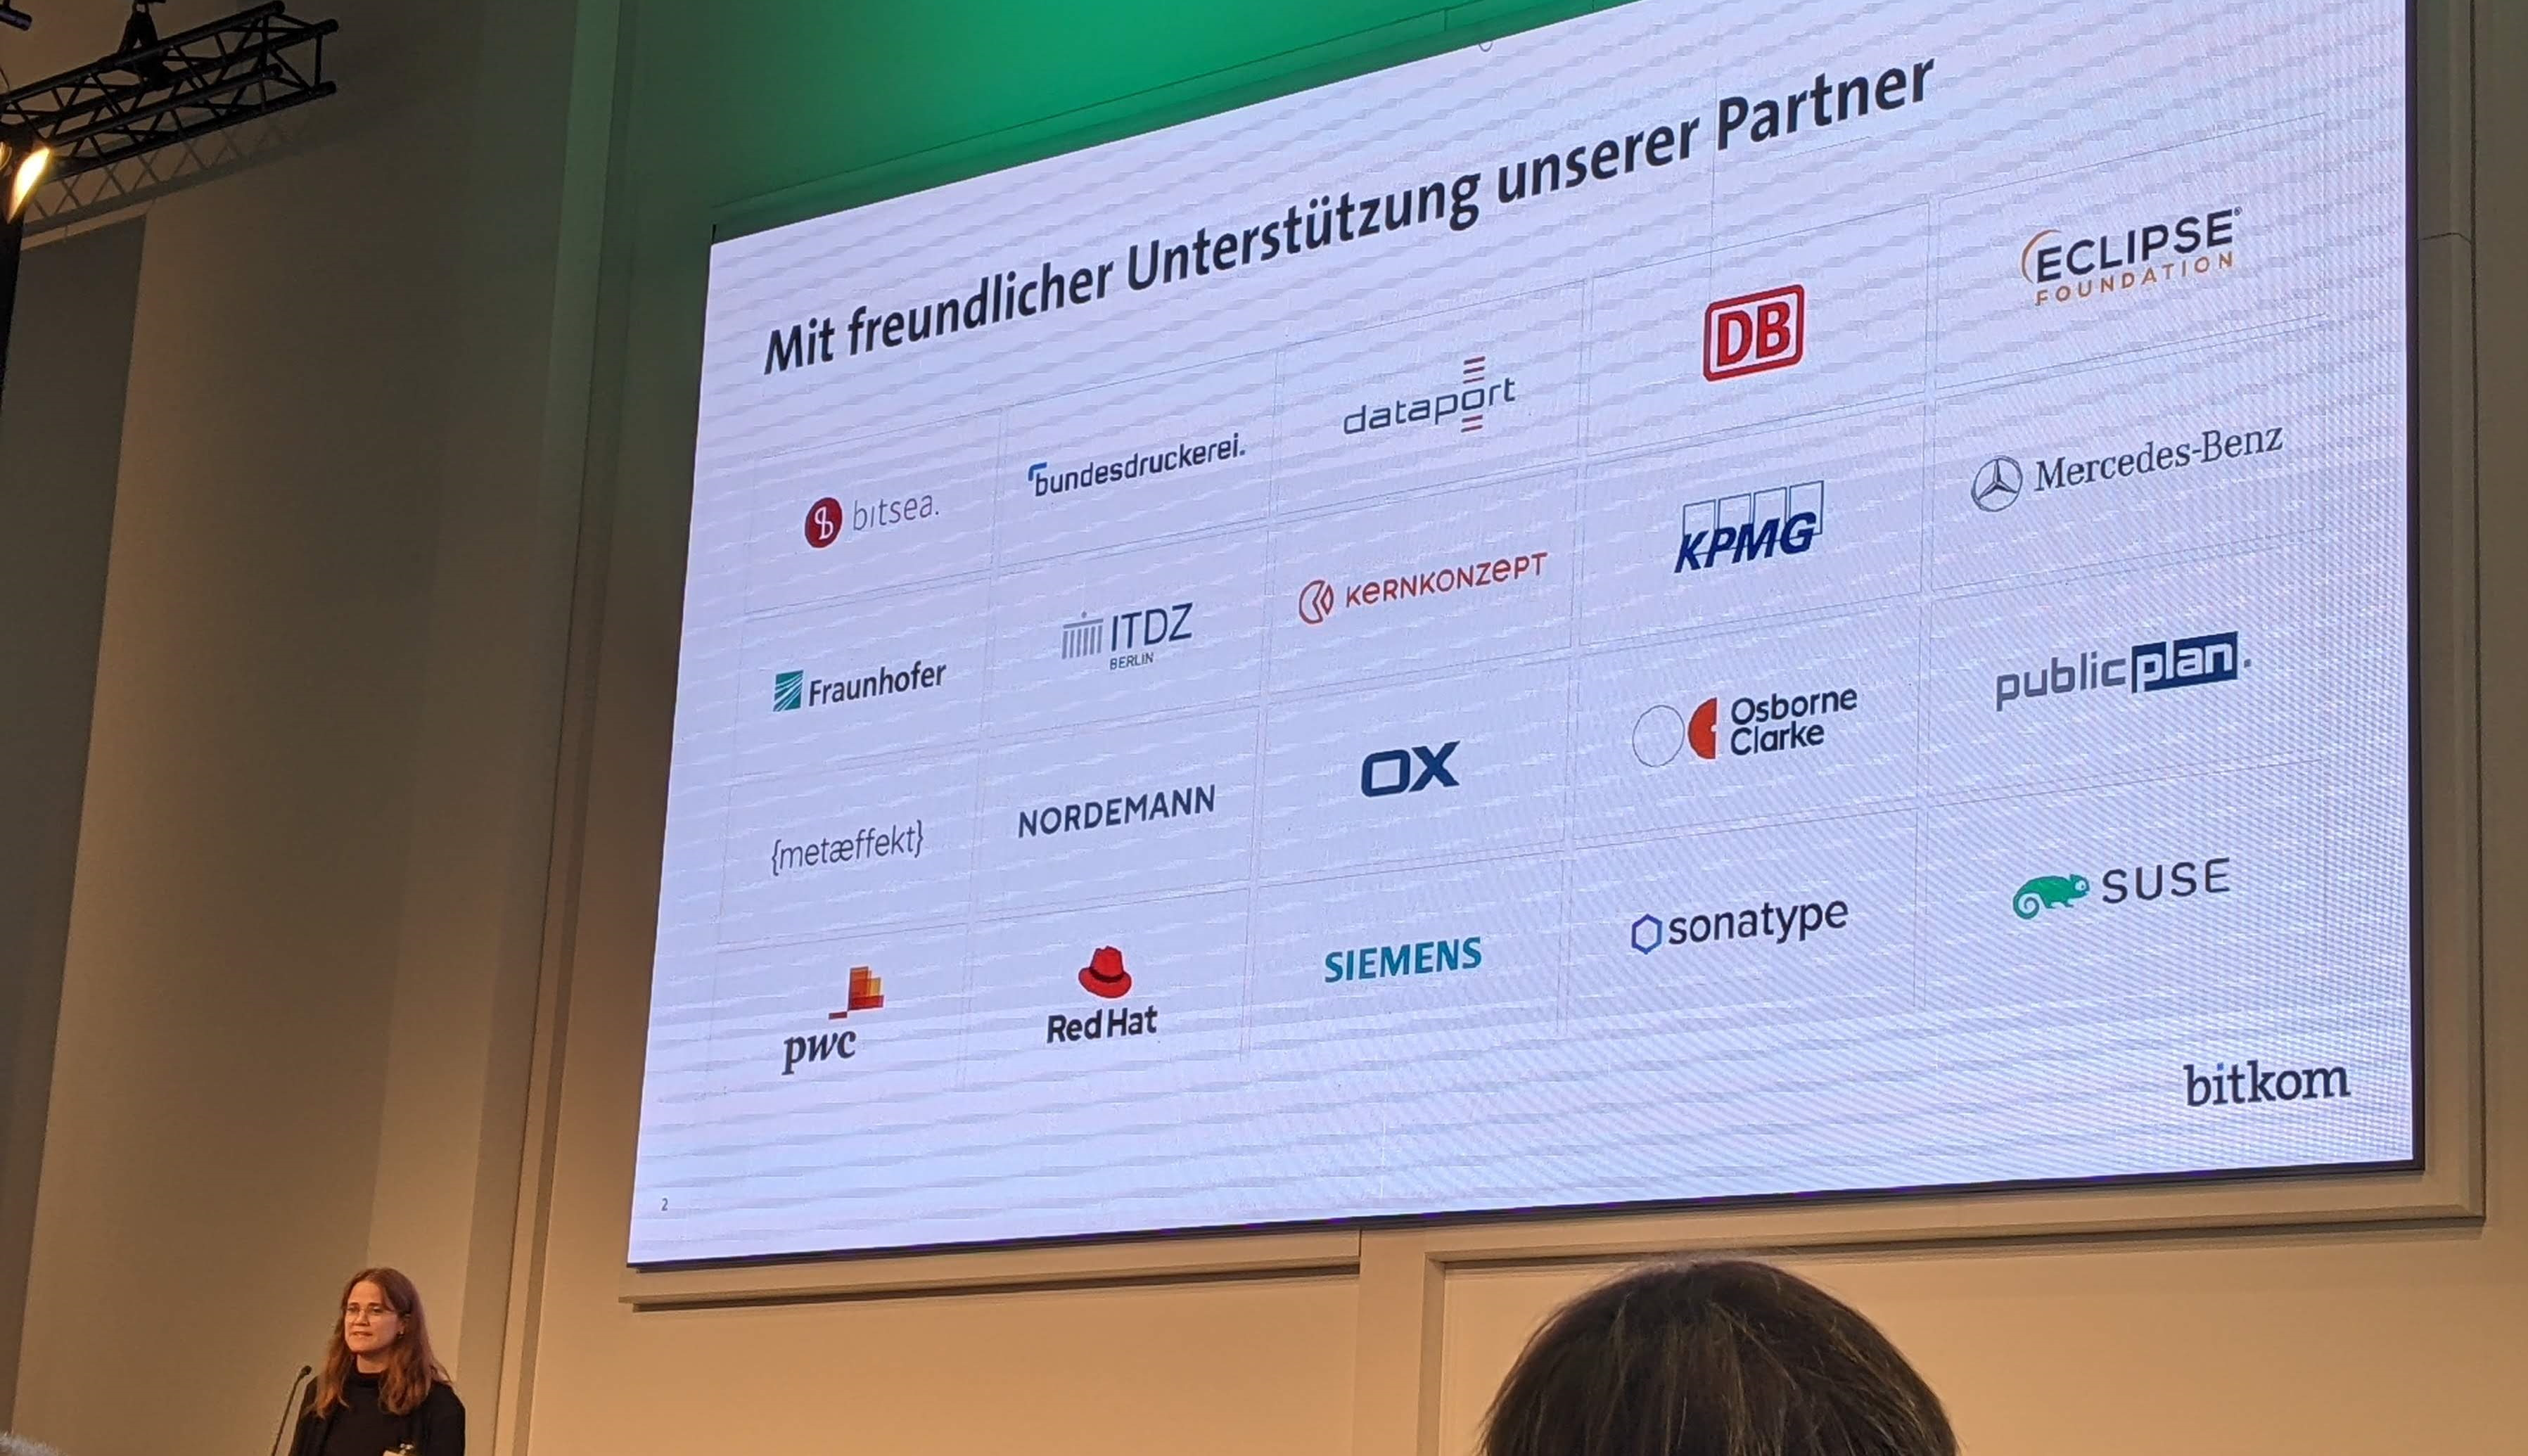
\includegraphics[width=0.8\textwidth, keepaspectratio]{res/img/2023-10-19-ak-os-metaeffekt-sponsor}
    \caption{Die {\metaeffekt} ist links als Sponsor zum OpenSource Monitor aufgeführt}
    \label{fig:foss23-sponsor-metaeffekt}
\end{figure}

\sweekdaymarginpar{\weekdayThursdayShort, \weekdayFridayShort}

Die Rückreise am Donnerstag verlief ohne Zwischenfälle, sodass der Freitag wieder der gewöhnliche Arbeitsalltag war.
Eine neue Kundenanforderung erforderte schon wieder direkte Aufmerksamkeit:
Einer unserer Download-Prozesse scheitert in ihrer Konfiguration, da der verwendete git-Befehl die konfigurierte Proxy-Informationen bislang scheinbar ignoriert.
Um das zu lösen, kann Git sowohl über einen Konfigurationsparameter im Befehlsaufruf, als auch über Umgebungsvariablen der Session konfiguriert werden.
Ich habe mich für die zweite Variante entschieden.

Ein persönliches Highlight war diesen Freitag allerdings, dass mein Bruder ab nächster Woche auch Teil des {\metaeffekt} Teams sein wird.


% Einarbeitung neuer Kollege (Nils)
\section{Woche 5 - Einarbeitung eines neuen Kollegen} \label{sec:bericht-wo-5}

% Woche 5 (2023-10-04 bis 2023-10-06)

\lweekdaymarginpar{\weekdayWednesdayLong}

Da Dienstag ein Feiertag war und ich montags einen Brückentag genommen hatte, war der Mittwoch mein erster Arbeitstag.
Die Einarbeitung meines neuen Kollegen war meine Hauptaufgabe für diese Woche.
Die Korrelationsdaten zu pflegen, also die Mappings zwischen unserer internen Darstellung von Software-Produkten und den Produkten in diversen externen Datenbanken, ist ab sofort sein Aufgabenbereich.
Passend dazu hat mein Chef uns einen neuen Datensatz gegeben, ein Inventar an Komponenten, den man einpflegen musste, anhand dem ich mit ihm die einfacheren Fälle und Grundlagen davon durchzugehen.

\sweekdaymarginpar{\weekdayThursdayLong}

Donnerstag habe ich erneut die etwas komplizierteren Fälle übernommen und ihn mit einigen einsteigerfreundlicheren versorgt.
Die Herausforderung für ihn als nicht-Informatiker an dieser Arbeit ist nicht nur die Methodik, sondern auch das gesammelte Wissen, das man über alle Software-Ökosysteme, Betriebssysteme und Software-Pakete haben muss.

\sweekdaymarginpar{\weekdayFridayLong}

Freitag habe ich ihm bereits etwas interessantere Fälle geben können und natürlich bei Fragen geholfen.
Ich bin etwas früher als er nach dem Weekly in das Wochenende gegangen.


% Weiter Daten-Korrelation & PowerShell Skripte
\section{Woche 6 - Daten-Korrelation \headerand PowerShell Skripte} \label{sec:bericht-wo-6}

% Woche 6 (2023-10-09 bis 2023-10-13)

\lweekdaymarginpar{\weekdayMondayShort\ - \weekdayWednesdayShort}

Da mein Kollege nicht das gesamte Inventar den Rest der Woche fertig bekommen würde, spielte sich diese Woche ähnlich wie letzte ab, in der ich meinen Kollegen bei der Arbeit unterstützte.
So konnte ich das Tool, das ich für diese Arbeit vor meinem Praktikum geschrieben hatte, selbst einmal anwenden und entdeckte einige Verbesserungsmöglichkeiten, die ich gleich umsetzte.
Das Tool (\qt{Correlation Utilities}) selbst ist Webapplikation, die mit einem lokal gehosteten Server, in Spring Boot implementiert, interagiert.
Das Ziel des Tools ist es, den Prozess des Mappings von unseren internen Produkten zu denen externer Datenbanken zu unterstützen.
Es aggregiert relevante Informationen automatisiert und macht Empfehlungen, wie am besten mit Fällen umgegangen werden sollte.
Dank des Tools besteht nun bereits fast keine Notwendigkeit, das ursprungs-Inventar zu durchsuchen oder Internet-Suchen zu starten.
Über die drei Tage habe ich es mit einigen weiteren Features erweitert.
Bis Mittwochabend hatten wir die Hälfte der Daten durchgearbeitet, den Rest sollte mein Kollege bis zum Ende der nächsten Woche erledigen.

\sweekdaymarginpar{\weekdayThursdayLong}

Donnerstag hatten mein Chef und ich morgens einen zweistündigen Termin mit einem unserer Kunden, {\aeclientZEZESE}, bei dem es um die automatisierte Erstellung einer SBOM (Software Bill of Materials) mit allen installierten Programmen, Treibern und Hardware-Devices auf Windows-Systemen ging.
Dieser Prozess sollte zweigeteilt sein:
Zunächst sollten über PowerShell-Skripte über Windows-Integrierte Features viele verschiedene Datenquellen angezapft und die rohen Ergebnisse in einem maschinenlesbaren Format in Dateien geschrieben werden.
Danach würde ein Maven-Plugin diese Daten analysieren und ein Inventar erzeugen.

Bis nächsten Montag sollten bereits erste Versionen der Skripte stehen.
Mein Arbeitslaptop selbst ist ein MacBook, also hat mir mein Chef einen zusätzlichen Windows-Laptop zum Entwickeln zur Verfügung gestellt.
An diesem habe mich zunächst einmal darüber informiert, wie man am besten an Windows-Systeminformationen gelangen kann.
Diese ersten Erkenntnisse habe ich zunächst in unserem internen Confluence niedergeschrieben, wo ich auch sonst meine Dokumentation ablege.

\sweekdaymarginpar{\weekdayFridayLong}

Freitag habe mich schnell wieder an das Thema gesetzt und mit den Ergebnissen meiner gestrigen Recherche angefangen, erste Skripte zur Sammelung von registrierten Programmen aus dem Store oder über Installers, die PNP-Devices (\qt{Plug and Play}) und Treibern.
Ich konnte die Hälfte der Use-Cases noch an diesem Tag durch verschiedene Skripte abdecken.


% PowerShell Skripte, Windows-Inventar & Strategieworkshop
\section{Woche 7 - Windows-Inventar-Extraktion \headerand Strategieworkshop} \label{sec:bericht-wo-7}

% Woche 7 (2023-10-16 bis 2023-10-20)

\lweekdaymarginpar{\weekdayMondayShort, \weekdayTuesdayShort}

Montag habe ich eine erste version der PowerShell Skripte fertigstellen können, die alle Use-Cases abdeckt.
Im Meeting später am Tag mit den Mitarbeitern von {\aeclientZEZESE} wurden meine Datensammlungs-Skripte dann live auf dem Ziel-Windows-Gerät erfolgreich ausgeführt.
Diese Daten auszuwerten hat gezeigt, dass sie noch nicht reichen, um ein vollständiges Bild zu erhalten, was ich dann den restlichen Tag durch Modifikationen an den Skripten geändert habe.

\sweekdaymarginpar{\weekdayWednesdayShort, \weekdayThursdayShort}

Die Entwicklung eines Java-Prozesses zur Verarbeitung von JSON-Daten aus PowerShell-Befehlen für ein Inventar im Format von {\metaeffekt} machte es nötig, die Ergebnisse der vielen verschiedenen PowerShell-Befehle zu kombinieren.
Wie bei Microsoft-Datenquellen so oft liefern die unterschiedlichen Befehle teils überlappende, teils einzigartige Datensätze, die nur zusammengenommen ein volles Bild ergeben.
Besonders bei Systeminformationen und PNP-Geräten waren Daten aus mehreren Befehlen zu konsolidieren.
Das Ergebnis war dann am Donnerstagabend ein vorläufiges Inventar, das zur Besprechung mit dem Kunden am Freitag noch etwas händisch aufbereitet wurde.

\sweekdaymarginpar{\weekdayFridayLong}

Der Freitag war ein ereignisreicher Tag:
Die {\metaeffekt} hat einen Strategieworkshop gehalten, der das Vorgehen der nächsten 9--12 Monate angeben sollte.
An einem großen Tisch und auf mehreren großen Whiteboard-Blättern wurden Wünsche und Pflichten aufgeschrieben und diskutiert.
Zu den Strategiepunkten, bei denen ich beteiligt sein werde, gehören:

\begin{smitemize}
    \item Eine Java-Implementierung von CVSS:2.0, CVSS:3.1 und CVSS:4.0 soll als Open-Source-Projekt auf GitHub veröffentlicht werden.
    Dazu muss die CVSS:4.0-Implementierung fertiggestellt und zusammen mit den anderen in unser Haupt-Repository verschoben werden.
    \item Ein Open-Source-Projekt, das den CVSS-Standard in den Versionen 2.0, 3.1 und 4.0 in TypeScript implementiert und damit auch im Web nutzbar ist, soll angelegt werden.
    Damit soll ein öffentliches Web-Interface erstellt werden, das die Berechnung und Modifikation von CVSS-Vektoren ermöglicht.
    \item Das interne Datenmodell, das für die Speicherung von Schwachstellen und Security Advisories verwendet wird, soll komplett neu geschrieben werden.
    Es soll mit diesem System zu jeder Zeit möglich sein, die exakte Quelle einer Schwachstelle und der von CVSS-Vektoren programmatisch zu identifizieren.
    \item Eine der Ausgaben unseres Systems ist ein sog. \qt{Vulnerability Assessment Dashboard} (VAD), was Ergebnisse aus dem Schwachstell-Monitoring mit aggregierten Details darstellt.
    Es soll nach der Neuentwicklung des Datenmodells in einer \qt{Generation 3.0} stark verändert werden, so sollen auch Kundenwünsche berücksichtigt werden.
\end{smitemize}

Das Meeting war sehr, hilfreich für mich, da es einen klaren roten Faden für das Semester vorgegeben hat.
Den Mitarbeitern von {\aeclientZEZESE} haben wir im Anschluss die Ergebnisse der Windows-Scans gezeigt und darum gebeten, dass sie die aktualisierten Skripte erneut ausführen, damit wir die vollständigeren Daten zu einem besseren Inventar umwandeln können.


% Abschluss Windows-Extraktion & Beginn Überarbeitung des Datenformats
\section{Woche 8 - Abschluss Windows-Extraktion \headerand Beginn Überarbeitung des Datenformats} \label{sec:bericht-wo-8}

% Woche 8 (2023-10-23 bis 2023-10-27)

\lweekdaymarginpar{\weekdayMondayShort, \weekdayTuesdayShort}

Mit den neuen Daten vom Freitag konnte ich Montag die Erkennung von Treibern, PNP-Devices und optionalen Features und die Performance des umfangreicheren Dateisystem-Scans einiger Skripte verbessern.
Um Dienstag die Windows-Extraktion vorerst abzuschließen, habe ich den restlichen Tag noch die PowerShell-Skripte unter einer MIT-Lizenz auf GitHub veröffentlicht und ein Maven-Plugin für die Inventar-Extraktion in Java geschrieben.

\sweekdaymarginpar{\weekdayWednesdayShort, \weekdayThursdayShort}

Mittwoch konnte ich (endlich) mit der Neuimplementierung der Datenstruktur und Logik dahinter beginnen.
Die einzelnen Tasks, die damit einhergehen, würden mich also die nächsten Wochen beschäftigen.
Bevor ich tatsächlich etwas programmieren konnte, wollte ich meine geplanten Änderungen in unserem internen Wiki dokumentieren und planen:
Begonnen habe ich mit dem Einführen eines Systems, das eine Quelle und Version eines Vektors eindeutig angeben kann.
Details dazu können in Kapitel \ref{subsec:projektbericht-loesungsweg-cvss-source-management} gefunden werden.
Eine erste Implementierung dazu konnte ich bereits Donnerstag fertigstellen.

\sweekdaymarginpar{\weekdayFridayLong}

Freitag habe ich damit verbracht, einem Kollegen zu helfen, der Probleme mit einer Software-Bibliothek hatte, die wir seit geraumer Zeit einsetzen.
Das Problem ließ sich am Ende auf einen internen Cache der Bibliothek zurückführen, den wir den Betreuern der Bibliothek in einem Issue\footnote{\url{https://github.com/spdx/Spdx-Java-Library/issues/215}} mitteilten.
Dieses Issue wurde einige Tage später durch einen Pull Request (PR) von meinem Kollegen behoben.


% Überarbeitung des Datenformats
\section{Woche 9 - Überarbeitung des Datenformats} \label{sec:bericht-wo-9}

% Woche 9 (2023-10-30 bis 2023-11-03)

\lweekdaymarginpar{\weekdayMondayLong}

Diese Woche begann ich mit dem nächsten Schritt, der Überarbeitung des Datenformats für Schwachstellen und Security Advisories.
Das bisherige Datenformat besteht im Wesentlichen aus einer \codendt{Map<List<Map<String, String>\!>\!>}, was das domänenspezifische Parsen der Werte erschwert, denn komplexe Attribute müssen so über mehrere Schlüssel verteilt sein.
Durch das Ein- und Auslesen dieser mehreren oder komplex strukturierten Felder entsteht ein zusätzlicher Komplexitätsaufwand, den man lieber vermeiden möchte.

\sweekdaymarginpar{\weekdayTuesdayShort, \weekdayThursdayShort, \weekdayFridayShort}

Nach der Fertigstellung der Planung der Implementierung in zwei Schritten am Montag konnte ich den Rest dieser Woche mit der Umsetzung in unserem internen Projekt, Artifact Analysis, starten.
Ich startete mit der Entwicklung von Wrapper-Klassen um die inneren \code{Map<String, String>} Strukturen, die die Map in eine Kollektion Instanzen unseres Datenmodells umwandeln.
Um diese Wrapper herum erstellte ich eine Verwaltungsklasse, die für die korrekte Initialisierung aller Wrapper-Instanzen zuständig ist, diese verwaltet und die Beziehungen zwischen ihnen modelliert.

Die Programmierung dieser Komponenten erfolgte \qt{blind}, da der Code aufgrund der vielen Änderungen nicht ausführbar war.
Daher musste ich warten, bis die Änderungen in Artifact Analysis umgesetzt waren, was Freitagnachmittag (\textit{fast}) der Fall war.
Durch ein längeres wöchentliches Meeting als sonst konnte ich die Umstellung nicht vollständig abschließen.


% Abschluss Überarbeitung des Datenformats und CVSS Implementierung Verschieben
\section{Woche 10 - Abschluss Überarbeitung des Datenformats \headerand CVSS Implementierung Refactoring} \label{sec:bericht-wo-10}

% Woche 10 (2023-11-06 bis 2023-11-10)

\lweekdaymarginpar{\weekdayMondayLong}

Den Montag habe also damit verbracht, die Änderungen am Datenmodell und die Integration in die Prozessschritte in Artifact Analysis mit dem letzten verbleibenden Prozessschritt, dem VAD, zu vervollständigen\@.
Da hier alle Daten aggregiert dargestellt werden, ist dies einer der komplizierteren Schritte.
Zuerst ging es nur darum, die alte Funktionalität mit dem neuen Modell wiederherzustellen, ohne die neuen Features, die dadurch ermöglicht werden.
Einige Stunden später konnte ich immerhin den Code wieder ausführen, allerdings traten einige erwartete Fehler auf, die ich den restlichen Tag bearbeitete.

\sweekdaymarginpar{\weekdayTuesdayLong}

Die nächsten Tage konnte ich mich auf das Verschieben der CVSS-Implementierungen aus Artifact Analysis nach Core, in ein separates Modul, kümmern.
Die Aggregation der mehreren CVSS-Vektor-Quellen war zwar abgeschlossen, nun musste allerdings noch ein Prozess entworfen werden, der die Auswahl effektiver Vektoren und das korrekte Kombinieren und Überlagern ermöglicht.
Mit der Auswahl effektiver Vektoren habe ich den gesamten Dienstag verbracht, doch mein initialer Ansatz war zu naiv gedacht, weswegen ich die folgenden Tage einen neuen Ansatz verfolgte.

\sweekdaymarginpar{\weekdayWednesdayShort, \weekdayThursdayShort}

Mit diesem neuen Ansatz habe ich mir etwas länger Zeit gelassen, mit einigen Schaubildern und Testfällen zur Unterstützung.
Donnerstagnachmittag war der CVSS-Selektor dann fertig - deutlich komplizierter als anfangs erhofft, aber er konnte alle relevanten Fälle abdecken.

\sweekdaymarginpar{\weekdayFridayLong}

Um die Selektor-Logik in die bisherigen Prozessschritte einfügen war eine Nutzer-Konfiguration nötig, in der diese definierbar sind.
Ich habe in unserer Codebasis bereits ein recht umfangreiches Konfigurationssystem gebaut, was ich sehr einfach auf diesen Anwendungsfall anpassen konnte.
Mit meinem Chef zusammen habe ich beschlossen, dieses Konfigurationsobjekt auf alle Attribute auszuweiten, die etwas mit Security zu tun haben.
Diese neue zentrale Stelle habe ich vor und nach dem Weekly begonnen, überall zu integrieren und die alten Konfigurationsparameter durch diese auszutauschen.


% Transferieren der Datenklassen nach Core
\section{Woche 11 - Transferieren der Datenklassen nach Core} \label{sec:bericht-wo-11}

% 2023-11-13 bis 2023-11-17

\lweekdaymarginpar{\weekdayMondayLong}

Ende letzter Woche hatte ich die CVSS-bezogenen Features implementiert und in den Anreicherungsprozess integriert, sodass das System nun CVSS-Vektoren von beliebigen Datenquellen aufnehmen und deren Quellen nachvollziehbar halten konnte.
Den Montag nutzte ich, um diese Vektoren und deren berechneten Scores im VAD auf eine angereicherte Art anzuzeigen, was erstaunlich gut funktionierte.

\sweekdaymarginpar{\weekdayTuesdayLong}

Dienstagmorgen besprach ich mit meinem Chef die Integration dieser Änderungen in den PDF-Report unseres Core-Projekts.
Wir entschieden uns dazu, vorläufig Teile der Klassen in das andere Projekt zu kopieren, um auch dort Zugriff auf die Parsing-Logik zu haben, was zwar nicht schön ist (Code-Duplizierung), aber für jetzt die einfachere Lösung ist.
Noch am Dienstag konnte ich die relevanten Klassen in das Core-Projekt übernehmen und testen, wobei ich eine Namenskonvention für die kopierten Klassen festlegte und jeweils deren ursprüngliche Herkunft vermerkte.

\sweekdaymarginpar{\weekdayWednesdayShort\ - \weekdayFridayShort}

Mittwoch und Donnerstag stellte sich heraus, dass der Austausch des Datenmodells hinter dem PDF-Report mit dem kopierten Datenmodell komplexer war als erwartet.
Ich musste einige Abschnitte im Datenmodell leider komplett neu implementieren.
Den Rest der Zeit konnte ich dann das aktualisierte Modell in den Report einbinden.

Wir verwenden Apache Velocity mit einem textbasierten Template-XML-Format, was die Integration des neuen Modells aus mehreren Gründen sehr zeitintensiv machte.
Bis Freitagmittag war die Migration des Reports noch nicht abgeschlossen, allerdings hat war am Nachmittag ein Meeting mit einer Mitarbeiterin von \aeclientZEZESE\ geplant, um die Nutzung unseres VADs und die Bewertung von Schwachstellen in ihren Systemen zu besprechen.
Als Vorbereitung erstellte ich eine HTML-Seite, die unsere verschiedenen öffentlichen JSON-Schema-Dateien dynamisch zusammenfasst.
Das Meeting verlief erfreulicherweise angenehm und war produktiv für beide Seiten.


% Integration des Datenmodells in PDF-Report
\section{Woche 12 - Integration des Datenmodells in PDF-Report} \label{sec:bericht-wo-12}

% 2023-11-20 bis 2023-11-24

\lweekdaymarginpar{\weekdayMondayLong}

Am Montag nahm ich mir eine kurze Auszeit von der Report-Migration und wendete mich einem anderen Aspekt des Refactorings zu:
Dem Tracking der genauen Matching-Konfigurationen von Schwachstellen, die aus verschiedenen Quellen identifiziert wurden.
Bisher beschränkt sich unser System auf das Tracking der \qt{CPE}-Informationen, allerdings ohne die dazugehörigen Versionsbereiche und auch nur bei diesen, nicht anderen Quellen.
In der Vergangenheit war das ausreichend, da nur die NVD als Datenquelle diente, aber mittlerweile kommen auch GitHub, Microsoft und andere hinzu.

Deshalb verbrachte ich den Tag damit, diese Daten in den verschiedenen Anreicherungsschritten in das von vor zwei Wochen implementierte Tracking-System einzupflegen.
Diese Informationen konnte ich noch am Montag in das VAD integrieren.
Bei dieser Gelegenheit wurde mir erneut bewusst, wie viel einfacher Anpassungen am VAD im Vergleich zum PDF-Report sind.

\sweekdaymarginpar{\weekdayTuesdayShort, \weekdayWednesdayShort, \weekdayThursdayShort}

In der Mitte der Woche konnte ich mich wieder vollständig auf die Integration des Modells in den Report konzentrieren.
Dieser Prozess ist stets gleich: Für jedes der etwa 20 Velocity-Templates in unserem Prozess überprüfe ich den alten Datenzugriff und suche ich im neuen Modell nach einem entsprechenden Zugriff oder implementiere neue Methoden.
Diese Änderungen mache ich entweder in den Adapterklassen, die als Schnittstelle zwischen Report und Modell dienen, oder direkt im Modell selbst.
In letzterem Fall muss ich die Änderungen sowohl in Core als auch in Artifact Analysis vornehmen.

Eine zusätzliche Herausforderung war, dass ich immer wieder auf Templates stieß, die ich zuvor noch nie gesehen habe und die ich erst verstehen musste.
Um nicht bei jedem Test den Dita-Renderingprozess starten zu müssen, nutze ich das Tool \qt{OxygenXML}, das eine Live-Preview ohne Stilelemente erlaubt.
Dennoch dauert es immer eine Weile, bis ich meinen Testdatensatz angepasst habe, um all diese Dokumente richtig testen zu können.

\sweekdaymarginpar{\weekdayFridayLong}

Freitag begann mit einer unerwarteten Anfrage meines Chefs:
Er fragte mich, ob ich Interesse hätte, alleine an einem Workshop zum CSAF-Standard\footnote{\url{https://web.archive.org/web/20240121120954/https://www.allianz-fuer-cybersicherheit.de/Webs/ACS/DE/Netzwerk-Formate/Veranstaltungen-und-Austausch/CSAFversum/CSAFversum_node.html}} (Common Security Advisory Framework) teilzunehmen, der vom Bundesamt für Sicherheit in der Informationstechnik (BSI) in München organisiert wird.
Nach einer kurzen Recherche zu CSAF fand ich heraus, dass es sich dabei um ein Schema handelt, ähnlich wie OSV\footnote{\url{https://osv.dev}}, das es Herstellern ermöglicht, Security Advisories und Informationen zu Schwachstellen in ihren Produkten zu veröffentlichen.

Der Hintergrund dieser Anfrage war, dass mein Chef plant, dass ich diesen Standard irgendwann in unser System integriere.
Da ich sowohl die Integration von CSAF als sinnvoll erachte, als auch persönlich mich auf eine Reise nach München freuen würde, stimmte ich dem Vorschlag zunächst einmal zu.

Den Rest des Freitags habe ich eine weitere Anfrage meines Chefs bearbeitet:
Das Anlegen von Korrelationsdaten für ein dringendes Inventar.
Dieser Prozess ist nicht besonders spannend, daher war ich froh, nach dem wöchentlichen Meeting ins Wochenende starten zu können.


% Fertigstellung der Integration des Datenmodells & Dokumentation
\section{Woche 13 - Fertigstellung der Integration des Datenmodells \headerand Dokumentation} \label{sec:bericht-wo-13}

% 2023-11-27 bis 2023-12-01

\lweekdaymarginpar{\weekdayMondayShort, \weekdayTuesdayShort}

Gegen Ende der letzten Woche fiel es mir zunehmend schwer, mich auf den Report zu konzentrieren.
Die Pause am Wochenende war anscheinend hilfreich, denn bis Dienstagabend konnte ich nach diesen zwei Wochen die Integration in den Report fast vollständig abschließen.
Ich musste natürlich auch hier noch neue Segmente in den Templates anlegen, die die Herkunft einer Schwachstelle erklären können, wie ich es auch schon im VAD getan hatte.

\sweekdaymarginpar{\weekdayWednesdayShort, \weekdayThursdayShort}

Am Mittwoch startete ich motiviert in den Tag, da nur noch wenige Schritte bis zur Fertigstellung des neuen Prozesses fehlten.
Dazu zählten vor allem die Übersichtsdiagramme mit verschiedenen Statistiken über die gefundenen Schwachstellen, die sowohl im VAD als auch im PDF-Report dargestellt werden.
Im VAD verwenden wir dafür ChartJs\footnote{\url{https://www.chartjs.org}}, während für den PDF-Report SVG-Charts mit JFreeChart\footnote{\url{https://www.jfree.org/jfreechart}} während der Dashboard-Generierung gerendert werden.

Ich stellte schnell fest, dass nie genau definiert wurde, welche Diagramme welche Werte aus welchen Quellen darstellen sollen und wie diese Werte gemappt werden.
Diese Unklarheit erschwerte es mir, die Diagramme im neuen Prozess zu replizieren, da ich die genauen Datenquellen erst durch Reverse-Engineering ermitteln musste.
Bevor ich also mit der Implementierung anfing, begann ich, ein wenig Dokumentation zu diesem Thema zu verfassen.
Tatsächlich konnte ich diese Arbeit bis später am Donnerstag abschließen und hatte damit das große Thema des Refactorings des Datenmodells quasi abgeschlossen.

\sweekdaymarginpar{\weekdayFridayLong}

Weil mir in den vergangenen Tagen die Wichtigkeit von Dokumentation wieder einmal aufgefallen war, nutzte ich den Freitag, um im internen Wiki einen \qt{Migrationsguide} zu erstellen.
Dieser dokumentiert alle Änderungen zwischen der alten und der neuen Generation unseres Systems und enthält zusätzliche Informationen zu einzelnen Themen.
Dazu gehören der Refactor der CVSS-Implementierung mit Unterstützung für mehrere Vektoren gleicher Art, die sonstige Erweiterung der Prozesse um CVSS, das Tracking der Herkunft von CVSS-Vektoren und Schwachstellen, das neue Datenmodell für Schwachstellen und Security Advisories, die zentrale Security Policy Konfiguration, neue Namenskonventionen, geändertes Verhalten und vieles mehr.

Im Weekly Meeting konnte ich berichten, dass der neue Prozess nahezu abgeschlossen ist.
Obwohl es noch einige Monate dauern wird, bis die ersten Kunden diesen nutzen, ist es immer ein gutes Gefühl, ein solches Projekt abzuschließen.


% Neuer Kollege, automatische Korrelationsdaten & Validierung des neuen Prozesses
\section{Woche 14 - Neuer Kollege, automatische Korrelationsdaten \headerand Validierung des neuen Prozesses} \label{sec:bericht-wo-14}

% 2023-12-04 bis 2023-12-08

\lweekdaymarginpar{\weekdayMondayLong}

Der Montag war auch der erste Arbeitstag eines neuen Kollegen, der uns bei der Entwicklung einer CI-Pipeline und eines Testing-Frameworks unterstützen sollte.
Ich half ihm vormittags bei der Einrichtung seines Laptops und erklärte ihm unsere Codebasis.
Nachmittags widmete ich mich einem anderen Kollegen, um über seine Änderungen an den Korrelationsdaten zu gehen, was den Rest des Tages in Anspruch nahm.

\sweekdaymarginpar{\weekdayTuesdayLong}

Diese gestrige Session mit den Korrelationsdaten erinnerte mich an die Art und Weise, wie wir Java-Versionen mit diesem System erkennen und, dass es nur ein provisorisches System sein sollte.
Ich entwarf Dienstag also ein System, das automatisch Korrelations-Einträge für alle bekannten Java-Versionen generieren kann.
Nach drei erfolglosen Iterationen über dieses Problem fand ich dann eine akzeptable und funktionierende Lösung und stellte sie dem Kollegen und meinem Chef vor.


\sweekdaymarginpar{\weekdayWednesdayShort, \weekdayThursdayShort}

In den folgenden Tagen nahm ich einen Schritt zurück, um den Refactoring-Prozess des Datenmodells noch einmal zu überprüfen.
Ich stellte fest, dass ich zwei größere Klassen vergessen hatte zu überführen und korrigierte zudem noch einige Fehler, die im Vergleich zu Generation 2 zu (zu stark) abweichenden Ergebnissen führten.
Nach diesen Korrekturen waren die Ergebnisse verbessert, und ich konnte endlich Generation 3 des Vulnerability-Monitorings meinem Chef präsentieren und besprechen.

\sweekdaymarginpar{\weekdayFridayLong}

Der bevorstehende CSAF-Workshop nächste Woche rückte näher, darum widmete ich den Freitag der Recherche über CSAF, indem ich die Dokumentation und einige Beispiele ansah.
Meine Erkenntnisse fasste ich in einem neuen Wiki-Artikel zusammen, wurde jedoch durch kleinere Anfragen und das wöchentliche Meeting immer wieder unterbrochen.
Die Recherche würde ich in der nächsten Woche fortsetzen.


% CSAF-Workshop in München
\section{Woche 15 - CSAF-Workshop beim BSI} \label{sec:bericht-wo-15}

% 2023-12-11 bis 2023-12-15

\lweekdaymarginpar{\weekdayMondayShort\ - \weekdayWednesdayShort}

Die Woche begann ich mit der Recherche zu CSAF, wobei ich mit der offiziellen Dokumentation\footnote{\url{https://docs.oasis-open.org/csaf/csaf/v2.0/os/csaf-v2.0-os.html}} begann.
Den Großteil der Zeit habe ich mich mit den JSON-Strukturen, Rollen der Teilnehmer, dem Produkt-Matching und den anderen Konzepten, die hinter CSAF stehen, beschäftigt.
Mir fielen einige Unterschiede zu anderen Standards auf, wie zum Beispiel, dass CSAF nicht nur das Format der Security Advisories definiert, sondern auch deren Veröffentlichung, Bereitstellung, Aktualisierung und Verarbeitung durch Endnutzer.
Diese Erkenntnisse hielt ich in einem Wiki-Eintrag fest und bereitete mich Mittwoch auf die Reise vor.

\sweekdaymarginpar{\weekdayThursdayLong}

Donnerstagmorgen reiste ich früh um 5:45 mit dem ICE zum Information Security Hub (ISH) des BSI am Flughafen München, wo der Workshop stattfand (Abbildung \ref{fig:yan-ish-csaf-muenchen}).

\begin{figure}[htbp] % here, top, bottom, separate page
    \centering
    
\includegraphics[width=0.4\textwidth, keepaspectratio]{res/img/2023-12-14-yan-vor-dem-ish-muenchen}
    \caption{Vor dem \qt{Information Security Hub} am Münchner Flughafen}
    \label{fig:yan-ish-csaf-muenchen}
\end{figure}

Vor dem Workshop nutzte ich die Gelegenheit, mich mit anderen Teilnehmern von Bosch und anderen Unternehmen auszutauschen.
Der Workshop selbst war eine Mischung aus theoretischen Präsentationen und praktischen Übungen.
Es ging um die Begriffe, Rollen und Abläufe, aber auch um das tatsächliche Einsetzen der bereitgestellten Tools, dem eigenen erstellen von Security Advisories und dem Veröffentlichen dieser.
Besonders interessant waren für mich die Diskussionen über die Produktidentifikation und dem CVSS-Standard.
Nach dem Workshop und weiteren Gesprächen am abschließenden Buffet beendete ich den Tag mit einem Telefonat mit meinem Chef.

\sweekdaymarginpar{\weekdayFridayLong}

Freitag setzte ich die Teilnahme am Workshop fort, heute war der Fokus auf der praktischen Anwendung des CSAF-Standards.
Ich konnte, nachdem ich die Aufgaben recht schnell abschließen konnte, anderen Teilnehmern dabei helfen, die weniger Informatiker sind als Planer und Manager.
Nach dem Workshop und abschließenden Gesprächen machte ich mich auf den Heimweg und kam sogar dank einer früheren Verbindung schneller nach Hause.
Meine ausführlichen Notizen und Überlegungen würde ich in der folgenden Woche präsentieren.


% Letzte Woche vor der Weihnachtszeit
\section{Woche 16 - Letzte Woche vor der Weihnachtszeit} \label{sec:bericht-wo-16}

% 2023-12-18 bis 2023-12-20

\lweekdaymarginpar{\weekdayMondayLong}

Im Gegensatz zum letzten Jahr, wo das Weihnachtsfest ins Neujahr zurückverschoben werden musste, fand das Weihnachtsfrühstück der \metaeffekt dieses Mal frühzeitig im Schwarzen Walfisch statt.
Nach diesem gemeinsamen Frühstück kehrten wir ins Büro zurück, wo ich einen kurzen Bericht über den CSAF-Workshop für unsere Website verfasste\footnote{\url{https://metaeffekt.com/\#news}} und mit dem neuen Kollegen ein Testkonzept für unseren Software-Scanner diskutierte.

\sweekdaymarginpar{\weekdayTuesdayShort, \weekdayWednesdayShort}

Die restlichen Tage vor dem Urlaub widmete ich mich dem Abschluss des Refactorings meines Datenmodells, einschließlich Dokumentation und Code-Aufräumarbeiten.
Nach einem ausführlichen Gespräch mit meinem Chef über den Workshop konnte ich den Pull Request für die dritte Generation unseres Vulnerability Monitoring Toolings fertigstellen.
Mittwochabend ging ich gemeinsam mit den Kollegen in die Weihnachtsferien.


% TypeScript CVSS Calculator
\section{Woche 17 - TypeScript CVSS Calculator} \label{sec:bericht-wo-17}

% 2024-01-08 bis 2024-01-12

\lweekdaymarginpar{\weekdayMondayLong}

Das neue Jahr begann mit der Aufgabe, einen CVSS-Rechner in TypeScript zu entwickeln, der dann in ein zu entwickelndes Web-Interface integriert werden soll.
Dieses Interface soll die Scores für beliebig viele Vektoren, unabhängig von ihrer Version, berechnen und visualisieren können.
Für das gesamte Projekt ist später eine Veröffentlichung unter einer Open-Source-Lizenz auf GitHub vorgesehen.
Am Montag richtete ich zunächst das Projekt auf unserem lokalen git-Server ein, bereitete einen Build-Prozess mit Webpack vor und legte leere Klassen und Interfaces an.

\sweekdaymarginpar{\weekdayTuesdayShort\ - \weekdayFridayShort}

Die restliche Woche übersetzte ich die Java-Implementierungen in TypeScript und nutzte Jest\footnote{\url{https://jestjs.io/}} für Tests.
Ich erstellte einen Datensatz von 20.000 Vektoren pro CVSS-Version mit ihren erwarteten Scores für automatisierte Tests, anhand denen ich die Implementierungen entwickelte.
Bis zum Ende der Woche hatte ich die Klassen für CVSS:2.0 und CVSS:3.0 fertiggestellt und begann Freitag noch mit der komplexeren Version CVSS:4.0, konnte sie aber noch lange nicht fertigstellen.


% CVSS Calculator Web UI
\section{Woche 18 - CVSS Calculator Web UI} \label{sec:bericht-wo-18}

% 2024-01-15 bis 2024-01-19

\lweekdaymarginpar{\weekdayMondayShort, \weekdayTuesdayShort}

Den Beginn der Woche verbrache ich damit, die Implementierung von CVSS:4.0 abzuschließen.
Im Vergleich zur offiziellen JavaScript-Referenzimplementierung\footnote{\url{https://github.com/RedHatProductSecurity/cvss-v4-calculator/blob/main/app.js}} ist mein Ansatz in TypeScript deutlich objektorientierter und meiner Meinung nach übersichtlicher.
Dazu habe ich einen eher ungewöhnlichen Ansatz gewählt:
ich übertrug die Java-Klassen erst einmal 1:1 in TypeScript und passte sie dann Stück für Stück an die Zielsprache an.
Zirkuläre Referenzen löste durch mit madge\footnote{\url{https://www.npmjs.com/package/madge}} erzeugten Visualisierungen.

\sweekdaymarginpar{\weekdayWednesdayShort\ - \weekdayFridayShort}

Nachdem alle Tests bestanden waren, implementierte ich das Web-Interface mit Bootstrap\footnote{\url{https://getbootstrap.com/}} und ChartJs.
Ich erstellte eine HTML-Struktur und entsprechendes JavaScript, um mit der CVSS-Bibliothek oder der NVD-API zu interagieren.
Nach der Basisfunktionalität verbesserte ich das UI, fügte Lizenzinformationen hinzu, räumte die Bibliothek auf und erstellte Dokumentation.
Das Ergebnis kann in Abb. \ref{fig:metaeffekt-cvss-calculator-ui} gesehen werden.
Das Projekt veröffentlichte ich auf GitHub\footnote{\url{https://github.com/org-metaeffekt/metaeffekt-universal-cvss-calculator}} und teilte es auf LinkedIn\footnote{\url{https://www.linkedin.com/feed/update/urn:li:activity:7151175714694729728/}}.
Das Feedback von unseren Kunden war sehr positiv, mit vielen interessanten Verbesserungsvorschlägen.

\begin{figure}[htbp] % here, top, bottom, separate page
    \centering
    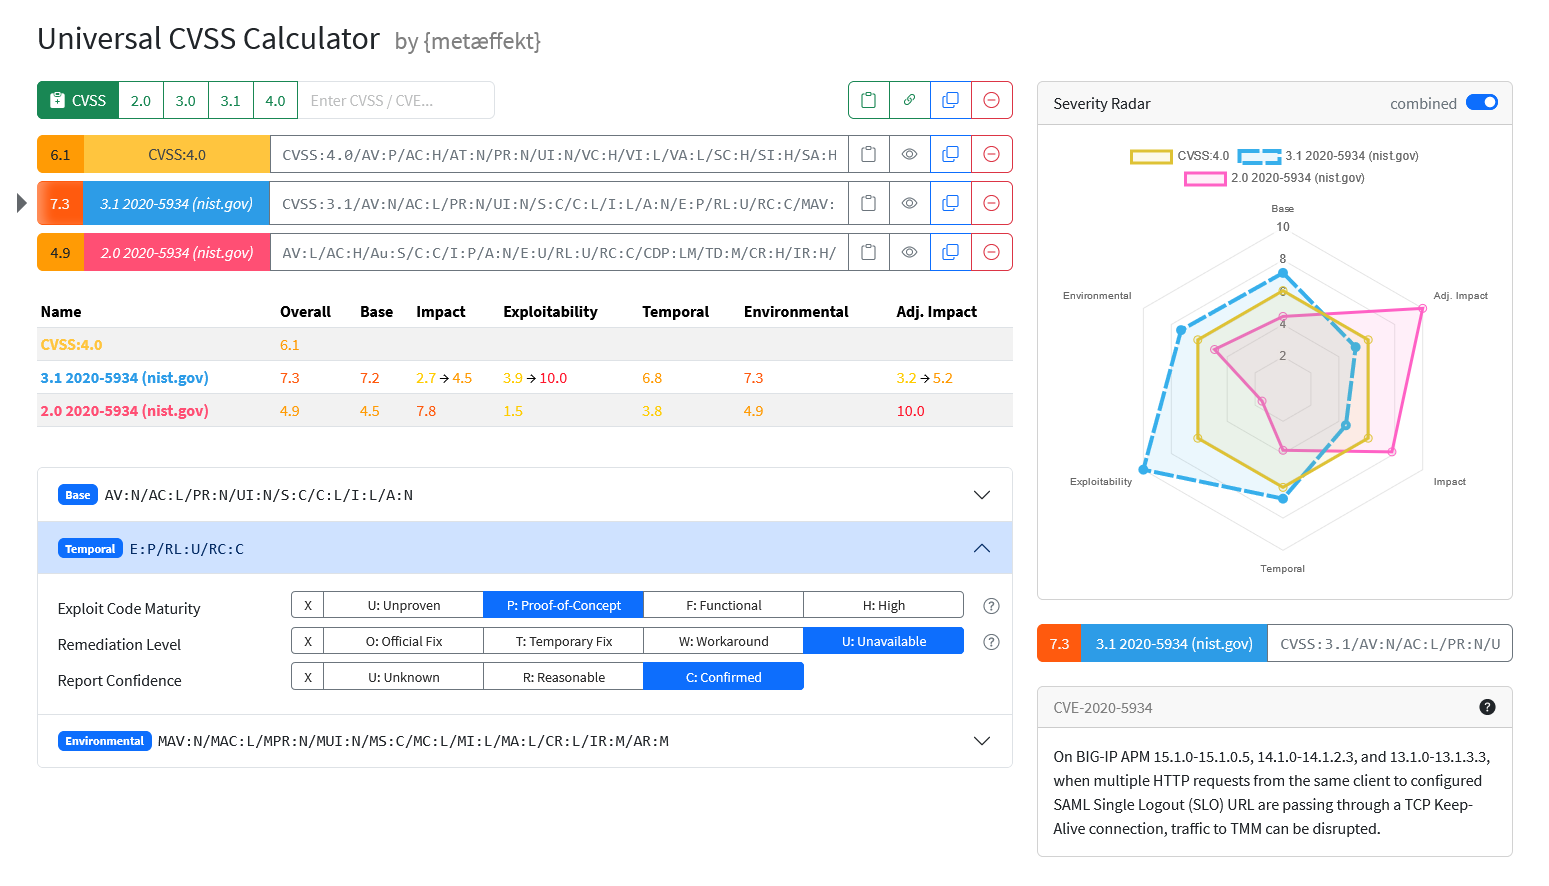
\includegraphics[width=0.8\textwidth, keepaspectratio]{res/img/metaeffekt-cvss-calculator-ui}
    \caption{Der {\metaeffekt} Universal CVSS-Rechner}
    \label{fig:metaeffekt-cvss-calculator-ui}
\end{figure}

Von Shane Coughlan, OpenChain General Manager und ein Referent des Open Source Forum der bitkom, haben wir freundlicherweise folgendes Zitat zu unserem Rechner erhalten:

\begin{quote}
    \textit{\qt{Contextualizing security threats is as important as identifying their existence,” says Shane Coughlan, OpenChain General Manager. “The emergence of open source tools to visualize this is a key part of ensuring the supply chain can plan ahead and action responses. We are delighted to see the work by Metaeffekt, an official OpenChain Partner, in the domain. It aligns well with OpenChain ISO/IEC 18974, the international standard for open source security assurance.}}
\end{quote}


%
\section{Woche 19 - Assessment-Policy \headerand Generation 3 Fertigstellung} \label{sec:bericht-wo-19}

% 2024-01-22 bis 2024-01-26

\lweekdaymarginpar{\weekdayMondayShort, \weekdayTuesdayShort, \weekdayWednesdayShort}

Einer der Kunden der \metaeffekt, den wir mit dem Schwachstell-Monitoring betreuen, geht nun in eine Projektphase, in der er Einschätzungen für Schwachstellen und Maßnahmen für deren Mitigierung vergeben möchte.
Dazu planen sie interne Workshops verpflichtend für mehrere Abteilungen anzubieten, wobei wir sie natürlich unterstützen wollen.

Darum schrieb ich die erste Hälfte der Woche an einer Assessment-Policy als Ausgangspunkt für ihre Überlegungen.
In diesem 6 Seiten langen Dokument berühre ich die folgenden Punkte:
Was ist der allgemeine Prozess, Vulnerability Monitoring durchzuführen?
Wie kann mit CVSS ein kontextualisiertes re-Scoring stattfinden?
Was sind die einzelnen CVSS Metriken der verschiedenen Versionen, die (Kontext-weit) verändert werden können/sollten?
Wie vergibt man einen Status, Risiken und Maßnahmen?
Wie werden Schwachstellen am besten priorisiert?

\sweekdaymarginpar{\weekdayThursdayLong}

Zusammen mit einer Kollegin habe ich dieses Dokument Donnerstag noch einmal überarbeitet und an meinen Chef übergeben, der es auch noch einmal überarbeitet und dann mit unseren Kunden durchgesprochen hat.

\sweekdaymarginpar{\weekdayFridayLong}

Passend dazu war Freitag dann der Tag, an dem der große Pull Request mit der Generation 3 unseres Vulnerability Monitorings ge-merged wurde.
Uns ist es besonders wichtig gewesen, die Änderungen aus dieser Version noch vor den Workshops des Kunden anzuwenden, denn so müssen nicht gleich einen Monat später neue Kurse für die neue Version angeboten werden.
Diese Änderungen zum Kunden zu bringen würde aber erst nächste Woche geschehen.

Den restlichen Tag habe ich noch einige Änderungen aufgrund von Feedback, das wir erhalten haben, an unserem CVSS-Rechner gemacht.
Freitag war außerdem ein alter Kollege zu Besuch, der vor einiger Zeit aufgehört hatte, hier zu arbeiten.


%
\section{Woche 20 - BSI-Meeting \headerand Integration von Generation 3} \label{sec:bericht-wo-20}

% 2024-01-29 bis 2024-02-02

\lweekdaymarginpar{\weekdayMondayLong}

Montags fand mit dem BSI ein Meeting bezüglich des CSAF-Standards und unseres CVSS-Rechners statt, mit Thomas Schmidt\footnote{\url{https://www.it-meets-industry.de/de/referent-thomas-schmidt}}, welcher bereits Leiter des CSAF-Workshops in München Ende letzten Jahres war, und Herr Von Samson.
Nach einer Demo unseres Toolings konnten wir nicht nur zur CSAF-Integration, sondern auch zum CVSS-Rechner, einige Tasks ableiten.
Thomas Schmidt erstellte in den folgenden Tagen dazu noch einige Issues auf unserem GitHub-Repository.

\sweekdaymarginpar{\weekdayTuesdayShort, \weekdayWednesdayShort, \weekdayThursdayShort}

Die restliche Woche startete dann die Integration von Generation 3 unseres Monitorings bei den mehreren Projekten unserer Kunden, um alle einheitlich von Generation 1 und 2 auf die neueste Generation 3 zu heben.
Der Prozess beinhaltete die Aktualisierung der Versionen und vor allem der Konfigurationen zum neuen Format, wobei der zuvor verfasste Migrationsguide wirklich sehr hilfreich war.
Trotz zahlreicher Komplikationen waren bis Donnerstagnachmittag alle Projekte aktualisiert.

\sweekdaymarginpar{\weekdayFridayLong}

Freitag bearbeitete ich die Issues\footnote{\url{https://github.com/org-metaeffekt/metaeffekt-universal-cvss-calculator/issues?q=is\%3Aissue+is\%3Aclosed}} von Thomas Schmidt, wobei bis auf Issue \#2 (keine Rückmeldung von FIRST\footnote{\url{https://www.first.org/cvss}} bis Praktikumsende) keine Probleme auftraten.
Nach unserem Weekly gab es ein Meeting mit einem Kunden zur finalen Integration der Generation 3 in ihre Pipeline.


%
\section{Woche 21 - Praktikumsbetreuung \headerand Abschluss des Praxissemesters} \label{sec:bericht-wo-21}

% 2024-02-05 bis 2024-02-09

\lweekdaymarginpar{\weekdayMondayLong}

Die letzte Woche meines Praktikums sollte ich einen BOGY-Praktikanten bei uns betreuen und die Integration von Generation 3 bei den Kunden fertigstellen.
Mit dem Praktikanten übte Montag ich Programmierkonzepte in Java, da er hauptsächlich Testfälle für unseren Software-Scanner und Komponenten-Extraktor schreiben sollte.

\sweekdaymarginpar{\weekdayTuesdayLong}

Der Praktikant konnte Konzepte schnell aufnehmen und begann Dienstag bereits mit den Testfällen.
Parallel dazu löste ich ein Problem mit der Laufzeit von Generation 3, das durch einen Programmierfehler von durchschnittlich 10 Minuten in Gen.\ 2 auf über zwei Stunden in Gen.\ 3 angestiegen war.
Eine kleine Code-Änderung (die Umwandlung einer Liste in ein Set) reduzierte die Laufzeit auf zweieinhalb Minuten, was uns natürlich alle beruhigt hatte.

\sweekdaymarginpar{\weekdayWednesdayShort, \weekdayThursdayShort}

Mittwoch und Donnerstag behebte ich in einem Teams-Meeting in Live-Kooperation die letzten Probleme, sodass Generation 3 nun endlich überall vollständig integriert war.
Die restliche Zeit verbrachte ich mit dem Praktikanten und diversen Aufgaben.

\sweekdaymarginpar{\weekdayFridayLong}

An meinem letzten Tag brachte ich Kuchen mit und verteilte ihn beim Weekly und nach dem Meeting gingen wir gemeinsam Currywurst essen.
Ich behebte ein Issue mit einem unserer Reports, das durch die neue Filtermethode in Generation 3 entstanden war, und führte neue Parameter und alternative Report-Templates ein.
Der BOGY-Praktikant und ich beendeten mit dieser Woche unser Praktikum erfolgreich.
Ich arbeitete noch weitere 12 Tage bei dem Unternehmen und schloss einen weiteren Vertrag für weitere Zusammenarbeit ab.


    \else
    %! Author = Yan Wittmann


\chapter{Tätigkeitsbeschreibung} \label{ch:wochenberichte-initial}

Im Folgenden wird eine Beschreibung der Tätigkeiten über die Praktikumswochen gegeben.

% Einarbeitung in CVSS 4.0
\section{Woche 1 - Einarbeitung in CVSS 4.0} \label{sec:bericht-wo-1-initial}

% Woche 1 (2023-09-04 bis 2023-09-08)

\lweekdaymarginpar{\weekdayMondayLong}

Mein erster Arbeitstag im Praktikums bei der {\metaeffekt} fiel mit dem Ende der Sommerpause des Unternehmens zusammen.
Da ich bereits seit einiger Zeit im Unternehmen arbeite und ich meine eigenständigen Aufgabenbereiche habe, war eine Einführung für mich nicht notwendig.
Bei {\metaeffekt} ist mein Aufgabenbereich als Entwickler ein automatisiertes Vulnerability Monitoring für unsere Kunden in der Programmiersprache Java zu implementieren und zu betreuen.
Als Hauptverantwortlicher für dieses Gebiet bin ich darüber hinaus für den Kundenkontakt für Fragen, Anforderungen und Unterstützung zuständig.
Ich verbrachte den Montag damit, einige während der Sommerpause aufgetretene Fehler in den Systemen von Kundenprojekten zu korrigieren und Gespräche mit Kollegen zu führen, um anstehende Projekte und Aufgaben zu klären.

Ein wichtiges Thema war die anstehende Veröffentlichung des CVSS 4.0-Standards, die für den 31.\ Oktober 2023\footnote{\url{https://www.first.org/cvss/v4-0/}} geplant war.
Die Software-Implementierung der {\metaeffekt} ist bereits in der Lage, die Scores der CVSS-Versionen 2.0 und 3.1 zu berechnen, und wir müssen in der Lage sein, auch die neuen CVSS 4.0-Vektoren zu berechnen, sobald offizielle Datenquellen diese auch bei sich integrieren.
Mit meinem Chef und Betreuer für das Praktikum, Karsten Klein, habe ich zudem vereinbart, während meines Praxis-Semesters tägliche Meetings mit ihm abzuhalten.

\sweekdaymarginpar{\weekdayTuesdayLong}

Am Dienstag startete ich damit, die zu dem Zeitpunkt noch unfertige Dokumentation und Beispiele von CVSS 4.0 zu studieren.
Ich stellte schnell fest, dass es mehr Unterschiede als Gemeinsamkeiten zu den vorherigen Versionen gibt, insbesondere in Bezug auf die mathematischen Hintergründe.
Ich dokumentierte dennoch meine Erkenntnisse in unserem internen Confluence Wiki.
Auf dem offiziellen RedHat GitHub-Repository\footnote{\url{https://github.com/RedHatProductSecurity/cvss-v4-calculator}} fand ich den Quellcode einer Referenz-JavaScript-Implementierung, die noch sehr nützlich werden sollte.

\sweekdaymarginpar{\weekdayWednesdayLong}

Am Mittwoch begann ich mit einem ersten Versuch einer Implementierung der CVSS 4.0-Berechnungen.
Wie ich bereits gestern vermutet hatte, ist die Berechnung bei 4.0 mathematisch deutlich komplexer, mit Hamming-Distanzen zwischen Vektoren und der Interpolation und Skalierung von mehrdimensionalen Räumen, versehen.
Dank der RedHat JavaScript-Implementierung konnte ich Mittwoch das Grundgerüst für meine Implementierung in Java vorbereiten.

\sweekdaymarginpar{\weekdayThursdayLong}

Der Donnerstag startete mit der Behebung einer \qt{OutOfMemoryError}-Exception im Code eines unserer Reports in einem Kundenprojekt, die auftrat, wenn eine zu große Menge an Daten verarbeitet wurde.
Das Problem war, dass während der Serialisierung in ein HTML-Dokument das interne Modell (damit auch der Speicherbedarf) kurzzeitig dupliziert wurde.
Ich konnte das Problem lösen, indem ich einen FileAppender verwende, der den HTML-String des Reports direkt in eine Datei schreibt, anstatt ihn wie zuvor im Speicher zu halten.

Der Hauptteil meines Tages war jedoch der Untersuchung von CVSS 4.0 zugeordnet.
Leider musste ich im Verlauf feststellen, dass die Referenzimplementierung und die Spezifikation im aktuellen Zustand voneinander abweichen, was bei einem unveröffentlichten Standard zwar verständlich, aber nicht hilfreich ist.
Ich meldete dieses Problem zusammen mit inhaltlichen Fragen in einem GitHub-Issue\footnote{\url{https://github.com/RedHatProductSecurity/cvss-v4-calculator/issues/32}} und beendete den Tag mit einer teilweise funktionierenden Implementierung.

\sweekdaymarginpar{\weekdayFridayLong}

Am Freitag erhielt ich recht schnell eine Antwort auf meine Fragen:
Wie erwartet ist die Spezifikation veraltet und die Implementierung korrekt.
Mithilfe dieser Informationen konnte ich die Berechnungen fertigstellen und durch einen Test-Datensatz, den ich durch die Referenzimplementierung erzeugt habe, validieren.
Damit war der erste Teil dieses Tasks erledigt:
Als Nächstes wollte ich mein Verständnis für die Theorie hinter CVSS 4.0 verbessern und zudem musste die neue Version noch richtig in unsere Systeme integriert werden.

Freitagmittag findet bei der {\metaeffekt} ein wöchentliches Meeting statt, das als \qt{Weekly} bezeichnet wird.
Hier berichtete ich über meine Erfahrungen mit der Implementierung von CVSS 4.0 und hörte, was die anderen Teammitglieder in dieser Woche erreicht hatten.
So beendete ich meine erste Praktikumswoche.


% Vertiefung in CVSS 4.0 und Korrelationsdaten
\section{Woche 2 - Vertiefung in CVSS 4.0 \headerand Korrelationsdaten} \label{sec:bericht-wo-2-initial}

% Woche 2 (2023-09-11 bis 2023-09-15)

\lweekdaymarginpar{\weekdayMondayLong}

Ich verbrachte den Montag damit, die Spezifikation\footnote{\url{https://www.first.org/cvss/v4.0/specification-document}},
die Entwicklungsgeschichte\footnote{\url{https://www.first.org/cvss/v4.0/user-guide\#New-Scoring-System-Development}}
und den Code tiefergehender anzusehen, um zu verstehen, wie die Berechnung des Scores funktioniert.
Über den ersten Schritt der Berechnung mit den MacroVektoren hatte ich ein bereits ein gutes Verständnis, meine Unklarheiten lagen eher in dem zweiten Schritt mit der Interpolation zwischen den einzelnen MacroVektoren.
Ich konnte selbst nach einem ganzen Tag an Recherche keine zufriedenstellende Erklärung finden, wie die Berechnung in diesem Schritt funktioniert.

\sweekdaymarginpar{\weekdayTuesdayShort, \weekdayWednesdayShort}

In Abwesenheit eines Kollegen übernahm ich Dienstag seine Aufgabe, die Pflege von sog. \qt{Korrelationsdaten}, ein von uns gepflegter Datensatz, der Software-Komponenten automatisch Produkten in externen Datenbanken wie den CPEs der NVD\footnote{\url{https://nvd.nist.gov/products/cpe}} zuordnen kann.
Dazu konnte ich ein von mir entwickeltes Tool nutzen, das ich kurz vor meinem Praktikum als Web-UI über Spring Boot neu aufgesetzt hatte, basierend auf umfangreichem Feedback des Kollegen.

In den verbleibenden zwei Stunden diskutierte ich mit meinem Chef über das Abbilden von \qt{Vulnerability Chaining} in unseren Systemen – ein Thema, das wir auf Kundenwunsch in den kommenden Monaten angehen müssen, auch wenn es noch keine hohe Priorität hat.

\sweekdaymarginpar{\weekdayThursdayLong}

Da die Implementierung und Integration von CVSS 4.0 bis Wochenende abgeschlossen sein musste, musste ich mich mit den folgenden verbleibenden Aufgaben intensiv beschäftigen:

\begin{smitemize}
    \item Parsing der Vektoren aus verschiedenen Quellen/Formaten
    \item Korrektes Verarbeiten der Berechnung von Scores und Modifizieren von Vektoren
    \item Anzeigen der Ergebnisse in unseren HTML- und PDF-Reports
\end{smitemize}

Da keine externe Datenquelle bisher CVSS 4.0 Vektoren bereitstellt, basierten einige meiner Annahmen über deren Formate auf Vermutungen, die später eventuell noch angepasst werden müssen.
Ich nutzte den Rest des Tages, um viele Code-Muster, die ich aus der Referenzimplementierung übernommen hatte, durch Refactoring-Operationen eleganter und objektorientierter zu gestalten und Code zu deduplizieren.
Am Ende des Tages stellte ich Pull Requests für die drei betroffenen Code-Projekte fertig.

\sweekdaymarginpar{\weekdayFridayLong}

Freitag widmete ich mich erneut dem Verständnis von CVSS 4.0.
Unter anderem berechnete ich manuell mehrfach auf unterschiedliche Weisen die drei Beispiele der MacroVektor-Interpolation aus der Spezifikation, was mein Verständnis erheblich verbesserte.

Das Weekly am Ende des Tages dehnte sich von einer auf fast zweieinhalb Stunden aus, da nicht nur ich, sondern auch einige Kollegen, diese Woche viel erreicht hatten.


% Excel-Limitierungen & Präsentationsvorbereitung
\section{Woche 3 - Excel-Limitierungen \headerand Präsentationsvorbereitung} \label{sec:bericht-wo-3-initial}

% Woche 3 (2023-09-18 bis 2023-09-24)

\lweekdaymarginpar{\weekdayMondayLong}

Die Woche startete eher ruhig, darum konnte ich endlich einmal einige der Issues aus dem längeren Jira-Backlog abarbeiten.

Bei einem dieser Issues ging es darum, in unserem automatisierten CPE Matching-Algorithmus zwischen Hardware- und Software-Komponenten zu unterscheiden, sodass Softwarekomponenten nicht mehr Hardware-CPEs (und umgekehrt) zugeordnet werden würden, mit dem Ziel, weniger false-positives zu erzeugen.
Das Einzige, was ich hierfür noch benötigte, war ein Indikator, ob eine Komponente Hardware oder Software ist.
Diesen wollten wir durch eine Liste an Kategorien für Hardware ermöglichen, die für die einzelnen Komponenten vergeben werden können.

Der Detailgrad dieser Kategorien war bisher jedoch noch nicht geklärt.
Ich habe nach einiger Recherche drei Vorschläge für meinen Chef vorbereitet und zu zweit konnten wir uns recht schnell auf einen dieser einigen.
Leider hat durch eine davon deutliche abweichende Drittmeinung eines anderen Kollegen die Diskussion den gesamten restlichen Tag eingenommen.
Ohne eine Lösung zu finden, vertagten wir die Diskussion, bis jemand einen neuen Ansatz gefunden hat.

\sweekdaymarginpar{\weekdayTuesdayShort\ - \weekdayThursdayShort}

Die folgenden Tage konnte ich mich eine Aufgabe in unserem Core-Projekt angehen, die ich schon lange erledigen wollte:
Eine Verbesserung der Excel-Serialisierung und Deserialisierung unserer Software-Inventare.
Das Zeichenlimit von $32.767$\footnote{\url{https://support.microsoft.com/en-gb/office/excel-specifications-and-limits-1672b34d-7043-467e-8e27-269d656771c3}} Zeichen pro Excel-Zelle stellte uns vor Probleme, da unsere Daten oft dieses Limit überschreiten.
Der aktuelle Workaround teilt bereits in unserem Datenmodell diese Werte in mehrere Speicherbereiche auf, sodass beim späteren Serialisieren keine Probleme auftreten.
Das führt dazu, dass man nicht einfach so auf die betroffenen Felder in unserem Modell zugreifen kann, ohne speziell von dem Workaround Gebrauch zu machen.

Dies ist offensichtlich keine elegante Lösung, einige Probleme daran sind:

\begin{smitemize}
    \item Weiß jemand nicht von diesem Workaround, wird durch eine falsche Zugriffsart nur ein Bruchteil der Daten zurückgegeben.
    \item Das automatische Stylen der Excel-Zellen und Spalten funktioniert nicht richtig, da die Spalten aufgeteilt werden.
    \item Falls später ein weiteres Format mit einem niedrigeren Limit hinzugefügt werden soll, muss dieses Limit auch bei allen anderen Formaten so angewendet werden.
\end{smitemize}

Ich arbeitete also den Rest des Tages an einer eleganteren Lösung, die die Datenaufteilung direkt beim (De-)Serialisierungsprozess vornimmt und ein allgemeines Styling-Modell für Excel-Dokumente einführt, das leicht auf andere Formate anwendbar ist.

\sweekdaymarginpar{\weekdayFridayLong}

Freitagmorgen wurde ich von meinem Chef mit folgender Information überrascht:
Nächste Woche Dienstag und Mittwoch sollte mit ihm und einer Kollegin nach Erfurt auf das Treffen des Arbeitskreises OpenSource\footnote{\url{https://www.bitkom.org/Bitkom/Organisation/Gremien/Open-Source.html}} unter dem Thema \qt{Open-Source-Communities} und auf das darauf folgende Forum OpenSource\footnote{\url{htthttps://www.bitkom.org/bfoss23}} der {\bitkom} gehen.
Der eigentliche überraschende Punkt war, dass ich bei dem Treffen des Arbeitskreises eine 25-Minütige Präsentation vor 30 Leuten, unter anderem von RedHat, Siemens, DB Systel und anderen großen Unternehmen, über die \qt{Identifikation und Bewertung von Schwachstellen mit Inhalten aus öffentlichen Quellen} halten sollte.

Ich wurde hiermit etwas ins kalte Wasser geworfen, denn ich war noch nie auf einem solchen Treffen war und wusste nicht, wie eine solche Präsentation auszusehen hat.
Ich nahm mir den restlichen Tag für die Vorbereitung darauf.
Trotz der Unterstützung meines Chefs bei der Themenauswahl und Strukturierung, war klar, dass die Zeit knapp werden würde.
Ich schaffte es, die Präsentationsfolien weitestgehend zu erstellen, doch das Skript hatte ich gerade erst angefangen zu verfassen.

\sweekdaymarginpar{\weekdaySaturdayShort, \weekdaySundayShort}

Und so kam das erste Mal, dass ich an einem Wochenende für die {\metaeffekt} gearbeitet habe.
Das Wochenende verbrachte ich damit, ein 11-seitiges Skript für die Präsentation zu schreiben, die Folien weiter anzupassen und Punkte notiert zu notieren, die ich noch mit meinem Chef am Montag besprechen wollte.
Am Sonntagabend hatte ich ein ausführliches Skript, doch zugegebenermaßen fehlte mir noch etwas, um vollends zufrieden zu sein.


% AK OpenSource & OpenSource Forum Erfurt
\section{Woche 4 - AK OpenSource \headerand OpenSource Forum Erfurt} \label{sec:bericht-wo-4-initial}

% Woche 4 (2023-09-25 bis 2023-09-29)

\lweekdaymarginpar{\weekdayMondayLong}

Nach einer kurzen Nacht, in der ich die letzten Feinschliffe an meinem Präsentationsskript anwendete, besprach ich Montag mit meinem Chef noch die letzten Unklarheiten.
Eines meiner Probleme bis jetzt war ein spezifischer Teil der Präsentation, der über ein Thema ging, mit dem sich zwar mein Chef gut auskennt, ich allerdings sehr wenig.
Mein Chef übernahm glücklicherweise kurzerhand diesen Teil.
Den Rest des Tages nutzte also ich lieber im Home-Office, um in Ruhe die Präsentation zu üben und meine Reisetasche für die morgige Reise nach Erfurt zu packen.

\sweekdaymarginpar{\weekdayTuesdayLong}

Der Dienstag begann früh mit unserer Reise mit dem ICE nach Erfurt.
Während der Zugfahrt nutzten mein Chef und ich die Zeit für eine letzte Durchsprache unserer Präsentation.
Angekommen in Erfurt ging es direkt in den nahegelegenen Räumlichkeiten der DB Systel.
Dort gab es zunächst einige einleitende Worte und eine Vorstandswahl, bevor ich mit meiner Präsentation dran war.

Meine Kollegen vor Ort haben mich noch einmal ermutigt und trotz anfänglicher Nervosität verlief alles reibungslos:
Ich war gut vorbereitet, hatte die Präsentation gut geübt und die Themen, die ich vorstellte, gehören zu meinem täglichen Arbeitsbereich seit drei Jahren.
Ich brauchte mein Skript kaum und das Feedback war ausschließlich positiv, was mich sehr gefreut hat, denn ich wollte wirklich einen Mehrwert in diese Runde bringen.

Abends wurde vom {\bitkom} eine Stadtführung und ein gemeinsames Abendessen mit anderen Teilnehmern des OpenSource Forums des nächsten Tages organisiert, an welchen wir teilnahmen.
Dort, und bereits beim Arbeitskreis, konnten wir uns auch mit den anderen Teilnehmern austauschen.

\sweekdaymarginpar{\weekdayWednesdayLong}

Das OpenSource Forum der {\bitkom} bot dann eine entspannte Alternative zum vorherigen Tag, bei dem die Teilnehmer vielfältige Präsentationen verfolgen und sich untereinander auszutauschen konnten.
Besonders spannend waren die Einblicke in die Open-Source-Strategien großer Unternehmen wie SAP, Siemens und Mercedes.
Die Parallelen im Bezug auf die aktuellen Herausforderungen und Lösungsansätze für die Verwaltung von Schwachstellen und Lizenzen von Open-Source-Software in ihren Produkten und Projekten haben mich etwas überrascht und bestätigten die Relevanz unserer Arbeit.

\begin{figure}[htbp] % here, top, bottom, separate page
    \centering
    \includegraphics[width=0.5\textwidth, keepaspectratio]{res/img/2023-10-19-yan-ak-os}
    \caption{Auf dem Forum Open Source der Bitkom 2023}
    \label{fig:foss23-yan-initial}
\end{figure}

Ein großer Programmpunkt war auch der {\bitkom} OpenSource Monitor\footnote{\url{https://www.bitkom.org/opensourcemonitor2023}}, den die {\metaeffekt} gesponsert hat und damit einen Beitrag über den Cyber Resilience Act\footnote{\url{https://digital-strategy.ec.europa.eu/en/policies/cyber-resilience-act}} in diesem verfassen durfte.
Wir wurden auch auf der großen Leinwand aufgeführt, wie in Abbildung\ \ref{fig:foss23-sponsor-metaeffekt-initial} zu sehen ist.

\begin{figure}[htbp] % here, top, bottom, separate page
    \centering
    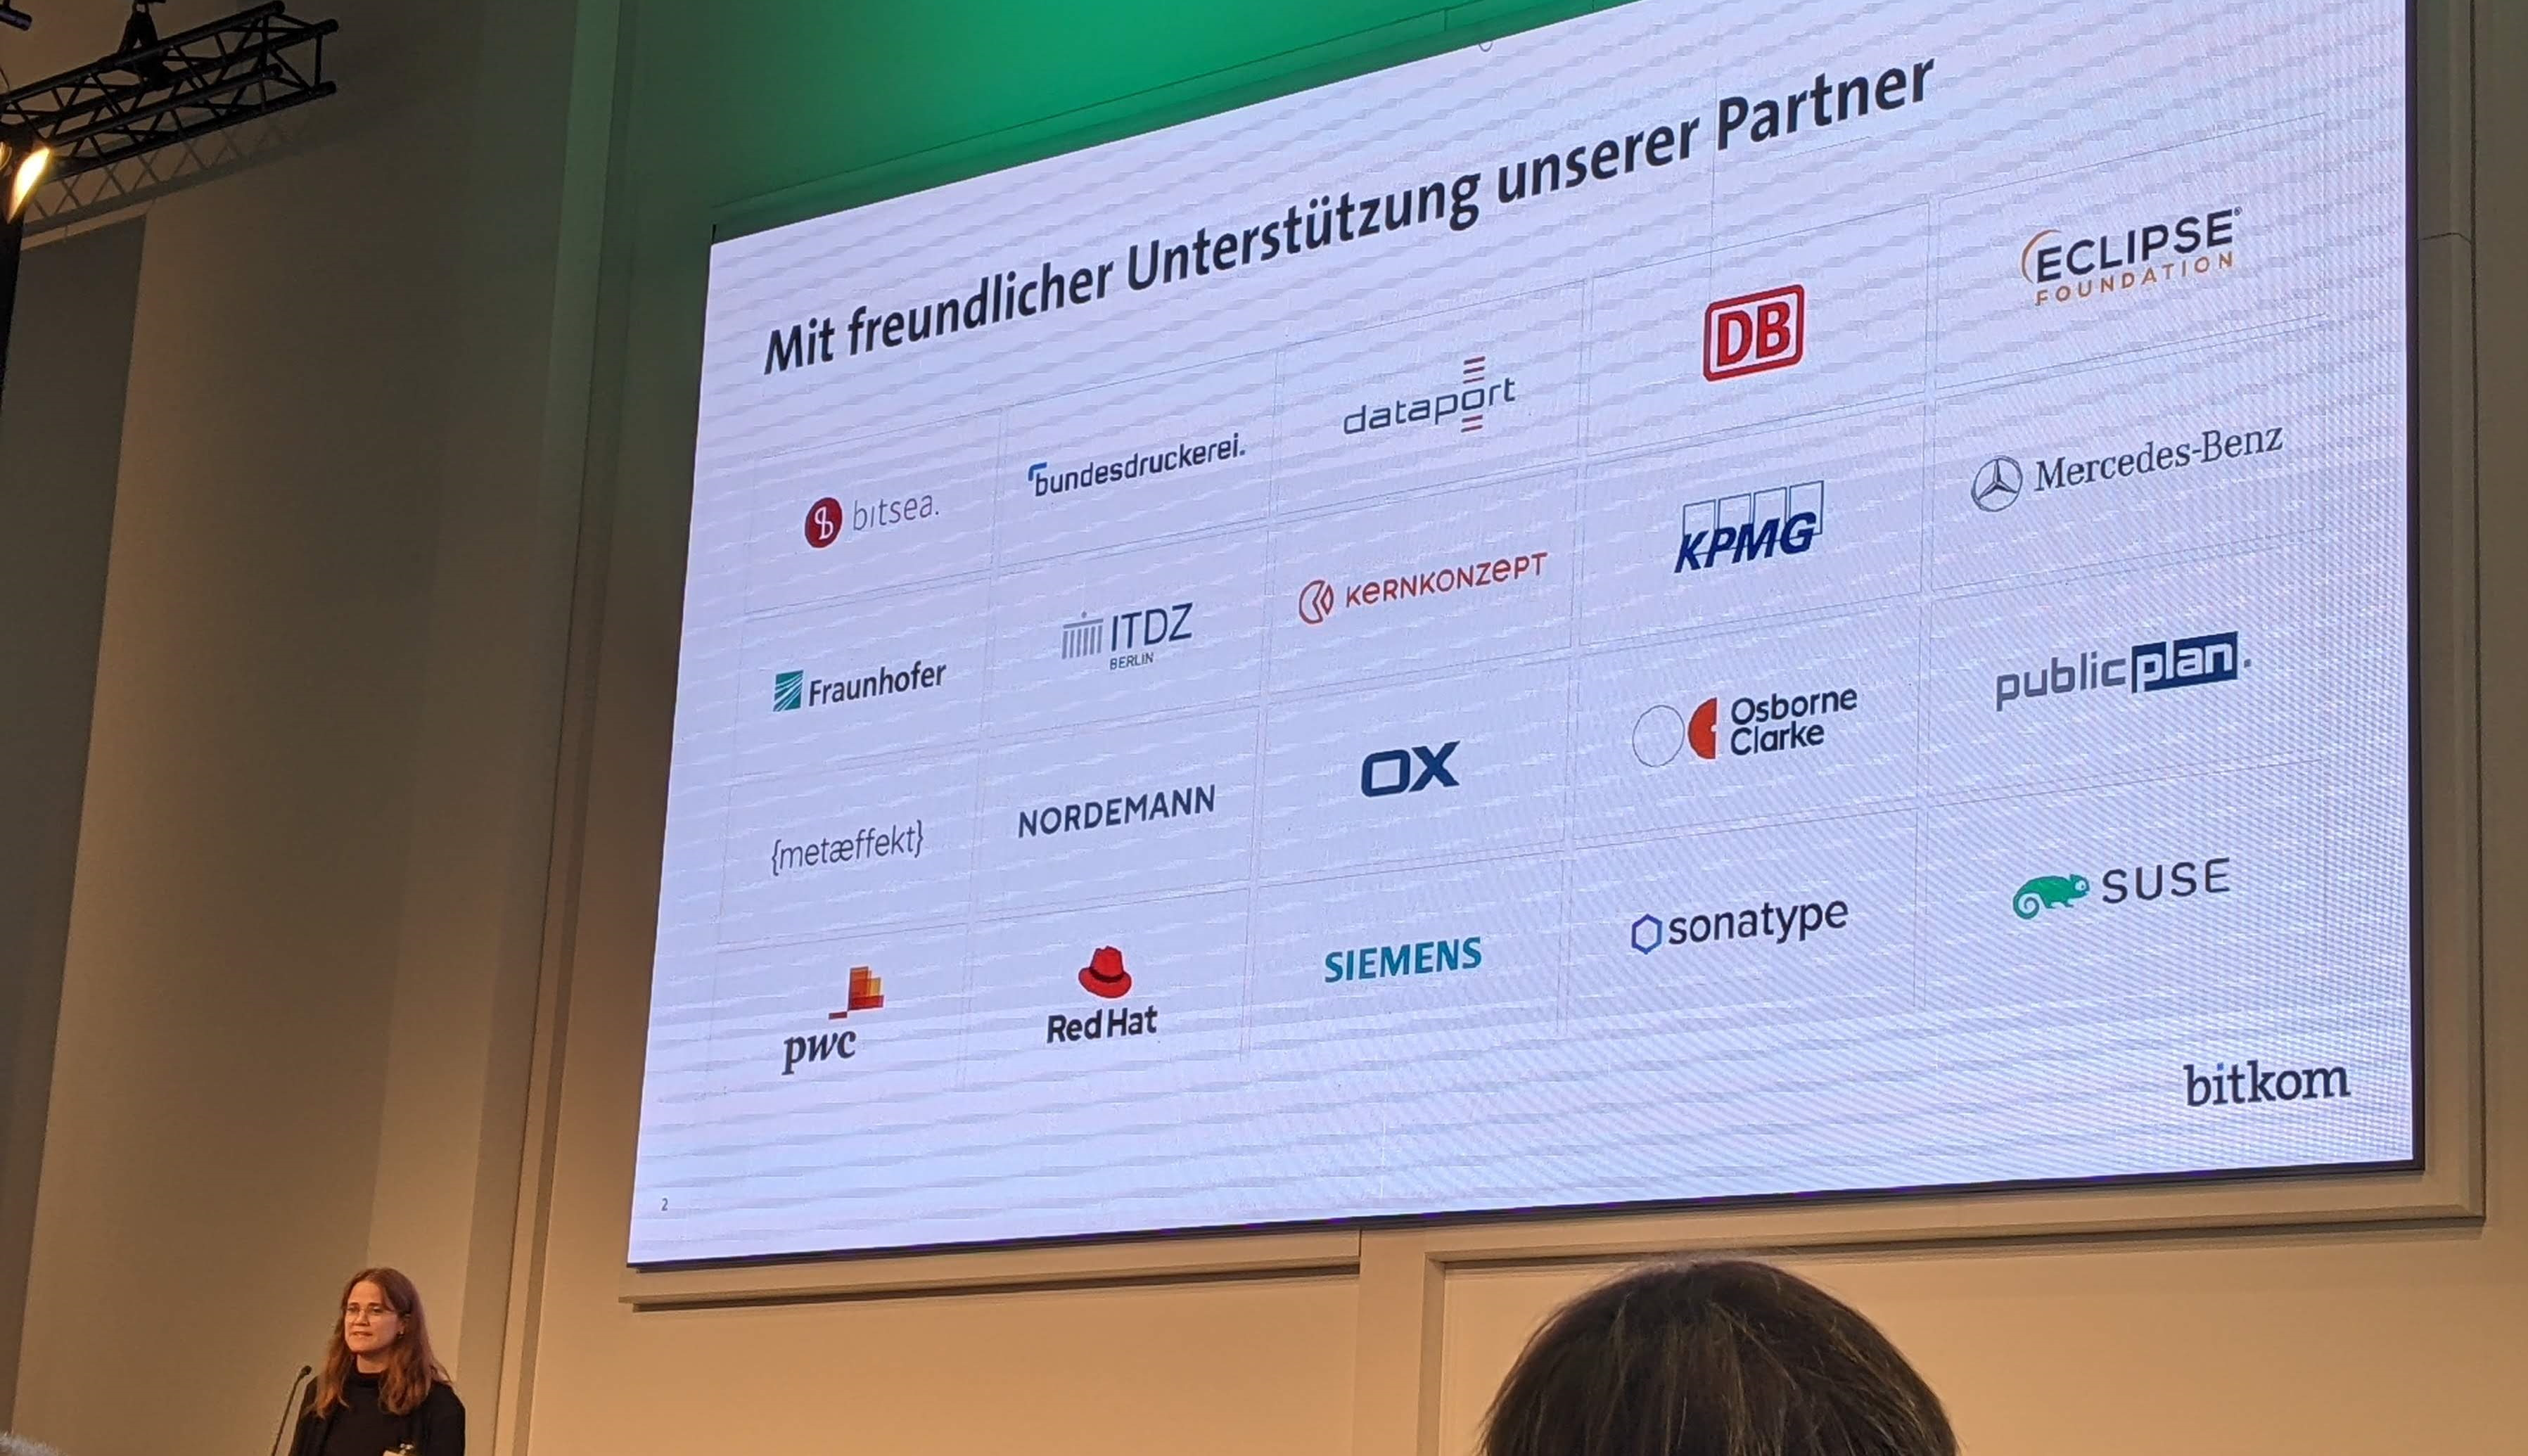
\includegraphics[width=0.8\textwidth, keepaspectratio]{res/img/2023-10-19-ak-os-metaeffekt-sponsor}
    \caption{Die {\metaeffekt} ist links als Sponsor zum OpenSource Monitor aufgeführt}
    \label{fig:foss23-sponsor-metaeffekt-initial}
\end{figure}

Es gab einige bekannte Gesichter vom vorherigen Tag, aber auch einige unserer direkten Kunden waren vertreten, die ich noch nie in Person getroffen hatte.
Außerdem hatte ich die fantastische Chance direkt mit Studenten und Angestellten verschiedener Unternehmen zu sprechen.

\sweekdaymarginpar{\weekdayThursdayShort, \weekdayFridayShort}

Die Rückreise am Donnerstag verlief ohne Zwischenfälle, sodass der Freitag wieder der gewöhnliche Arbeitsalltag war.
Eine neue Kundenanforderung erforderte schon wieder meine direkte Aufmerksamkeit:
Einer unserer Download-Prozesse scheitert in ihrer Konfiguration, da der verwendete git-Befehl die konfigurierte Proxy-Informationen bislang scheinbar ignoriert.
Um das zu lösen, kann Git sowohl über Umgebungsvariablen konfiguriert werden, als auch über einen Konfigurationsparameter im Befehlsaufruf.
Ich habe mich für die Umgebungsvariablen entschieden, die ich in der Prozess-Session, die über Java geöffnet wird, mit den Proxy-Informationen setzen kann.

Ein persönliches Highlight war diesen Freitag allerdings noch, dass mein Bruder nun auch Teil des Teams wird.
Über die letzten Tage hat er seine Bewerbung abgeschlossen, wurde angenommen und hat heute noch seinen Arbeitsvertrag unterzeichnet.
Er wird ab sofort die Korrelationsarbeiten des anderen Kollegen übernehmen.


% Einarbeitung neuer Kollege (Nils)
\section{Woche 5 - Einarbeitung eines neuen Kollegen} \label{sec:bericht-wo-5-initial}

% Woche 5 (2023-10-04 bis 2023-10-06)

\lweekdaymarginpar{\weekdayWednesdayLong}

Da Dienstag ein Feiertag war und die {\metaeffekt} Montag einen Brückentag hatte, war der Mittwoch der erste Arbeitstag diese Woche und vor allem der erste für meinen neuen Kollegen.
Die Einarbeitung von ihm war meine Hauptaufgabe für diese Woche.
Sein Aufgabenbereich wird es sein, die Korrelationsdaten, also die Mappings zwischen unserer internen Darstellung von Software-Produkten und den Produkten in diversen externen Datenbanken, zu pflegen.
Passend dazu hat mein Chef uns einen neuen Datensatz gegeben, ein Inventar an Komponenten, den man einpflegen musste.
Diese Daten sollten bis zum Ende der nächsten Woche fertig sein.
Den Tag habe ich dann also dazu verwendet, mit ihm die Grundlagen unseres Systems und die Benutzung der von mir geschriebenen internen Tools, durchzugehen.

\sweekdaymarginpar{\weekdayThursdayLong}

Der Kollege hatte beschlossen, in seiner ersten Woche mehr als seine 10 Stunden zu arbeiten, darum konnte ich ihn am Donnerstag gleich wieder im Büro begrüßen.
Wir haben uns an die Software-Inventare gemacht, bei denen ich die etwas komplizierteren Fälle übernommen habe und ihn mit einigen einsteigerfreundlicheren versorgt habe.
Die Herausforderung an dieser Arbeit ist nicht nur die Methodik, sondern auch das gesammelte Wissen, das man über alle Software-Ökosysteme, Betriebssysteme und Software-Pakete haben muss, um die richtigen Entscheidungen treffen zu können.
Genau dieses Wissen ist, was ihm noch fehlt, dennoch hat er sich für einen ersten Tag sehr gut geschlagen.

\sweekdaymarginpar{\weekdayFridayLong}

Freitag startete ich mit den Inventaren zunächst ohne meinen Kollegen, der erst zum Weekly dazu kommen konnte.
Dieses Mal habe ich habe ihm etwas interessantere Fälle gegeben und natürlich bei Fragen geholfen.
Dies war das Ende der ersten Woche für ihn, der allerdings noch etwas länger dort verblieben ist, da er erst etwas später dazugekommen ist.


% Weiter Daten-Korrelation & PowerShell Skripte
\section{Woche 6 - Daten-Korrelation \headerand PowerShell Skripte} \label{sec:bericht-wo-6-initial}

% Woche 6 (2023-10-09 bis 2023-10-13)

\lweekdaymarginpar{\weekdayMondayShort, \weekdayTuesdayShort, \weekdayWednesdayShort}

Der Anfang dieser Woche spielte sich ähnlich zur letzten ab: das Anlegen von Korrelationsdaten zu den neuen Inventardaten.
Da es absehbar war, dass die Menge nicht von meinem neuen Kollegen bis zum Ende der Woche alleine bewältigt werden konnte, sollte nun auch ich mich wenigstens teilweise daran beteiligen.

Intern betreiben wir auch gerne etwas, das sich \qt{Dogfooding} nennen lässt:
die von uns entwickelten Tools sollen wir auch selbst einmal anwenden, in der Hoffnung, dass Verbesserungsmöglichkeiten entdeckt und umsetzt werden, bevor man diese auf andere loslässt.
Dies war also ein Anlass für mich, meine eigenen Tools, die ich damals für den anderen Kollegen geschrieben hatte, den der neue Kollege inzwischen ersetzt hat, an einem echten Fall einzusetzen.
Ich habe diese Korrelationsarbeit schon immer zwar als interessant, jedoch auf Dauer auch etwas mühsam und monoton angesehen.
Daher habe ich dies gerne als Anlass genommen, etwas an dem Tool weiterzuentwickeln.

Nehmen wir dennoch einen Schritt zurück:
bei dem Tool, von dem ich berichte, handelt es sich um eine Webapplikation, die mit einem lokal gehosteten Spring Boot Server interagiert.
Bei dem Server wurde sich für Java entschieden, da die von der {\metaeffekt} produzierten Applikationen zum sehr großen Teil ebenfalls in Java geschrieben sind und deren Integration über eine einfache Dependency möglich war.

Das Ziel dieses Tools ist es, den Prozess des Mappings von unseren internen Produkten zu denen externer Datenbanken zu unterstützen:
es soll also möglichst alle Informationen zu Komponenten anzeigen, die automatisierbar abfragbar sind, und Empfehlungen machen, wie am besten mit einem Fall umgegangen werden sollte.

Bereits vor dem Erstellen des Tools war es klar, dass es viele verschiedene Workflows abbilden muss, eventuell auch welche, die zu dieser Zeit noch nicht bekannt waren.
Daher ist das Webinterface dank Gridstack\footnote{\url{https://gridstackjs.com/}} modular und mit den abgekapselten Funktionalitäten (\qt{Widgets}) kann über drag-and-drop ein beliebiges Layout erzeugt werden.
Einige der Widgets sind:
eine tabellarische Übersicht über die Komponenten in einem Inventar, eine Detailzone über die aktuell ausgewählte Komponente,
eine Query-View um den lokalen Index der Datenbanken zu aktualisieren und Abfragen darauf zu ermöglichen, eine Sicht,
in der die bereits erzeugten Korrelationsdaten automatisch nach Übereinstimmungen durchsucht werden und einigen weiteren.

Dank des Tools besteht nun bereits fast keine Notwendigkeit, das ursprungs-Inventar zu durchsuchen oder Internet-Suchen zu starten.
Jedoch, wie gesagt, ist es noch nicht perfekt und ich habe mich über die Tage also daran gemacht, einige spezifische Features, wie eine live-Aktualisierung der Korrelationsdaten auf die Komponenten und schlauere automatisierte Internet-Suchen hinzuzufügen.

Bis Mittwochabend hatten mein Kollege und ich die Hälfte der Daten durchgearbeitet und validiert, da ich jedoch den Rest der Woche wieder zu meinen eigentlichen Aufgaben zurückkehren musste, haben wir bereits mit meinem Chef ausgemacht, dass die Daten nicht bis Freitag fertig würden.

\sweekdaymarginpar{\weekdayThursdayLong}

Donnerstag hatten mein Chef und ich gleich morgens einen zweistündigen Termin mit einem unserer Kunden, {\aeclientZEZESE}, bei dem es um die automatisierte Erstellung einer SBOM (Software Bill of Materials),
beziehungsweise eines Inventars von allen installierten Programmen, Treibern und Hardware-Devices auf Windows-Systemen ging.
Am Ende der Videokonferenz war klar, dass der Prozess zweigeteilt sein wird:

Ein erster Schritt, bestehend aus PowerShell-Skripten, wird über Windows-Integrierte Features viele verschiedene Datenquellen anzapfen und die rohen Ergebnisse in einem maschinenlesbaren Format in Dateien schreiben.
Der zweite Schritt ist ein Maven-Plugin, das diese Daten analysiert und Komponenten in diesen erkennt.

Bis Montag sollten bereits erste Versionen der Skripte erstellt werden, darum habe ich mich gleich daran gesetzt.
Mein Arbeitslaptop ist ein MacBook, also hat mir mein Chef für diese Woche einen zusätzlichen Windows-Laptop zum Entwickeln zur Verfügung gestellt.

Das habe ich auch den restlichen Tag gemacht:
Ich habe mich zunächst einmal darüber informiert, was die Unterschiede der PowerShell zu anderen Terminals sind und wie man an Systeminformationen gelangen kann.
Meine ersten Ergebnisse habe ich in unserem internen Confluence niedergeschrieben, wo ich auch sonst meine Dokumentation ablege.

\sweekdaymarginpar{\weekdayFridayLong}

Freitag war ein intensiver Tag, denn ich bekam von meinem Chef die Information, dass wir bis Montagnachmittag bereits eine erste Version der Skripte fertig haben wollten.
Ich habe mich also schnell wieder an das Thema gesetzt und mit den Ergebnissen meiner gestrigen Recherche angefangen, erste Skripte zu schreiben.

Die Use-Cases sind das Sammeln von registrierten Programmen aus dem Store/über Installers, Sub-Trees von der Registry, eine Liste an Pfaden im Dateisystem, Systeminformationen wie die Windows-Version und installierte Patches, alle PNP (\qt{Plug and Play}) Devices und zuletzt alle installierten Treiber.

Es geht in diesem Schritt darum, erst einmal eine große Menge an Daten über das System zu sammeln, die dann im nächsten ausgewertet werden können.
Ich habe also mit Befehlen wie \code{Get-WmiObject} und seine über 1300 abfragbaren Datenklassen oder \code{Get-Computerinfo} etwas herumexperimentiert und tatsächlich fast die Hälfte der Use-Cases noch an diesem Tag durch verschiedene Skripte abdecken können.

Natürlich gab es auch wieder ein Weekly, bei dem ich über meine Erkenntnisse meinem Chef und Team-Mitgliedern berichten konnte.


% PowerShell Skripte, Windows-Inventar & Strategieworkshop
\section{Woche 7 - Windows-Inventar-Extraktion \headerand Strategieworkshop} \label{sec:bericht-wo-7-initial}

% Woche 7 (2023-10-16 bis 2023-10-20)

\lweekdaymarginpar{\weekdayMondayLong}

Montag stellte ich also eine erste, funktionierende Version der PowerShell Skripte fertig, die alle Use-Cases abdecken konnten.
Ich habe hier nach dem Prinzip \qt{Lieber zuviel als zu wenig} gearbeitet, habe also redundante und zusätzliche Informationen gesammelt, da das nächste Meeting erst wieder am Freitag sein wird und ich nicht darauf warten könnte.

Das Meeting mit den Mitarbeitern von {\aeclientZEZESE} verlief sehr gut:
Wir wurden live per Video-Call in das Test-Labor mitgenommen, wo das Ziel-Windows-Gerät vorhanden war.
Meine Skripte wurden auf dem System ohne Komplikationen ausgeführt und nach Besprechungen über das weitere Vorgehen haben wir diese Daten auch übermittelt bekommen.

\sweekdaymarginpar{\weekdayTuesdayLong}

Den Dienstag habe ich dann begonnen, die Daten zunächst manuell auszuwerten und musste, wie erwartet, feststellen, dass noch einige Daten für ein vollständiges Bild fehlen.
Vor allem zu den PNP-Devices gibt es im WMI-Interface sehr viele Subklassen, die je Details über eine gewisse Kategorie liefern können.
Die Skripte habe ich den Tag lang angepasst, sodass sie nun wirklich alle benötigten Daten abfragen.

\sweekdaymarginpar{\weekdayWednesdayShort, \weekdayThursdayShort}

Die folgenden beiden Tage habe ich damit verbracht, den zweiten Schritt der Windows-Inventar-Extraktion zu schreiben:
einen Java-Prozess, der die JSON-Daten verwertet und daraus ein Inventar im proprietären Format der {\metaeffekt} erzeugt.

Ich habe in der Vergangenheit bereits Erfahrungen mit Inkonsistenzen in den Datenquellen von Microsoft gemacht, wie denen zwischen dem
MSRC Security Update Guide\footnote{\url{https://msrc.microsoft.com/update-guide}},
MSRC CVRF API\footnote{\url{https://api.msrc.microsoft.com/cvrf/v2.0/swagger/index}} und
Security Update Catalogue\footnote{\url{httphttps://www.catalog.update.microsoft.com/Home.aspx}},
die jeweils ein unvollständiges Bild der Security-Situation rund um Microsoft geben und nur zusammen betrachtet vollständig sind.
Nicht anders war es hier:
die unterschiedlichen Befehle an die PowerShell liefern je Teile eines großen Bildes zurück, die sich gegenseitig ergänzen müssen.

Dies war vor allem bei den Systeminformationen und Informationen zu PNP-Geräten der Fall.
Bei den Systeminformationen bieten mindestens vier verschiedene Befehle (siehe Listing\ \ref{lst:win-systeminfo-commands-initial}) jeweils teils überlappende, teils einzigartige Datensätze an.
Die PNP-Geräte waren ähnlich:
Grundlegende Informationen können durch zwei Hauptbefehle abgerufen werden (siehe Listing\ \ref{lst:win-pnp-commands-base-initial}), für Details zu einzelnen Devices müssen jedoch viele verschiedene spezifische WMI-Klassen abgefragt werden (siehe Listing\ \ref{lst:win-pnp-commands-details-initial}).
Hier habe ich mindestens 20 weitere Klassen\footnote{Alle Klassen: \url{https://learn.microsoft.com/de-de/windows/win32/cimwin32prov/win32-provider}} abgefragt und die Daten in einen einheitlichen Datensatz konsolidieren können.

\begin{lstlisting}[language=PowerShell, label={lst:win-systeminfo-commands-initial}, caption={Windows Systeminformationen abfragen}]
Get-ComputerInfo
systeminfo
Get-WmiObject -Class Win32_ComputerSystem
Get-WmiObject -Class Win32_OperatingSystem
\end{lstlisting}

\begin{lstlisting}[language=PowerShell, label={lst:win-pnp-commands-base-initial}, caption={Windows PNP-Devices abfragen}]
Get-PnpDevice
Get-WmiObject -Class Win32_PnPEntity
\end{lstlisting}

\begin{lstlisting}[language=PowerShell, label={lst:win-pnp-commands-details-initial}, caption={Details zu Windows PNP-Devices abfragen}]
Get-WmiObject -Class Win32_Printer
Get-WmiObject -Class Win32_Processor
\end{lstlisting}

Natürlich habe ich auch die restlichen Daten noch verarbeitet und hatte zum Schluss über 30 verwendete PowerShell-Befehle, deren Daten ich zu dem Inventar umgewandelt habe.
Donnerstagabend hatte ich also einen Prozess und ein vorläufiges Inventar, das wir am Freitag mit dem Kunden besprechen konnten.

\sweekdaymarginpar{\weekdayFridayLong}

Dieser Freitag war ein ereignisreicher Tag:
Die {\metaeffekt} hat einen Strategieworkshop gehalten, der das Vorgehen der nächsten 9--12 Monate angeben sollte.
Auf diesen Tag hatte ich mich bereits seit einigen Wochen gefreut, da er jedes Jahr für mich und die anderen neue Aufgaben und einen roten Faden festlegt, der vor allem für mein Praxissemester dieses Halbjahr wichtig ist.

An einem großen Tisch und auf mehreren großen Whiteboard-Blättern wurden Wünsche und Pflichten aufgeschrieben und diskutiert.
Ein großer Punkt war dieses Mal:
Wenn wir nächstes Jahr in Erfurt auf der großen Bühne stehen, was wollen wir dort zeigen können?

Aus den Ergebnissen des Tages ließ sich auf jeden Fall ein roter Faden für mich herauslesen.
Zu den Strategiepunkten, bei denen ich beteiligt sein werde, gehören:

\begin{smitemize}
    \item Eine Java-Implementierung von CVSS:2.0, CVSS:3.1 und CVSS:4.0 soll als Open-Source-Projekt auf GitHub veröffentlicht werden.
    Dazu muss die CVSS:4.0-Implementierung noch fertiggestellt und zusammen mit den anderen in unser Haupt-Repository (Core) verschoben werden.
    \item Ein weiteres Open-Source-Projekt soll ebenfalls auf GitHub angelegt werden, das den CVSS-Standard in den Versionen 2.0, 3.1 und 4.0 in TypeScript implementiert und damit auch im Web nutzbar ist.
    Hiervon existiert noch nichts, sodass ich hier von Grund auf beginnen werde.
    \item Mit der TypeScript-Implementierung soll ein öffentliches Web-Interface erstellt werden, das die Berechnung und Modifikation von CVSS-Vektoren ermöglicht.
    \item Das interne Datenmodell, das für die Speicherung von Schwachstellen und Security Advisories verwendet wird, soll komplett neu geschrieben werden.
    Dabei sollen einige Redundanzen entfernt und die Datenstruktur sowohl für den Entwickler, als auch für den Nutzer einfacher und nachvollziehbarer werden.
    Nachvollziehbarkeit ist ein wichtiges Stichwort, denn es soll mit diesem System zu jeder Zeit möglich sein, die exakte Quelle einer Schwachstelle und von CVSS-Vektoren zu programmatisch identifizieren.
    \item Eine der Ausgaben unseres Systems ist ein sog. \qt{Vulnerability Assessment Dashboard} (VAD), für welches ich vor einigen Jahren den Code einer \qt{Version 1} und \qt{Version 2} geschrieben hab.
    Es stellt die Ergebnisse aus dem Schwachstell-Monitoring in einem übersichtlichen Dashboard mit aggregierten Details dar.
    Dieses VAD soll im Anschluss an die Neuentwicklung des Datenmodells ebenfalls neu geschrieben werden, da mit der Zeit viele mögliche Verbesserungen aufgekommen sind.
    Bei dieser \qt{Version 3.0} des VAD sollen auch Kundenwünsche berücksichtigt werden.
    \item Das letzte Ziel wird nicht mehr in meinem Praxissemester gestartet:
    Es soll ein Software-Asset Monitoring implementiert werden, das über einzelne Software-Artefakte hinausgeht und Aussagen über ganze Software-Produkte treffen können soll.
    Dazu soll ebenfalls ein Reporting und Dashboard erstellt werden, dieses Mal wird es allerdings kein alleinstehendes Dokument, sondern bekommt ein Backend in Java.
\end{smitemize}

Hier haben wir zum Schluss eine große Timeline gezeichnet, die sich in mehrere Stränge aufteilt.
Diese Stränge bestehen aus mehreren Schlüsselpunkten, an denen der Fortschritt gemessen werden kann.
Diese Timeline hing bis zum Ende meines Praxissemesters noch dort und war immer nützlich, um zu sehen, wie weit auch andere sind.

Natürlich war dies nicht der einzige Tagespunkt, denn den Mitarbeitern von {\aeclientZEZESE} haben wir unsere Ergebnisse der Windows-Scans gezeigt und darum gebeten, dass sie die aktualisierten Skripte erneut ausführen, damit wir vollständigere Daten erhalten.
Dieses Meeting war allerdings recht schnell vorbei.


% Abschluss Windows-Extraktion & Beginn Überarbeitung des Datenformats
\section{Woche 8 - Abschluss Windows-Extraktion \headerand Beginn Überarbeitung des Datenformats} \label{sec:bericht-wo-8-initial}

% Woche 8 (2023-10-23 bis 2023-10-27)

\lweekdaymarginpar{\weekdayMondayLong}

Durch einige neue Anforderungen an die Windows-Extraktion, die ich am Freitag erhalten hatte, habe ich die Woche mit der Anpassung der Skripte und der Inventar-Generierung begonnen.
Vor allem ging es um die (genauere) Erkennung von Treibern, PNP-Devices, optionalen Features und einen umfangreicheren Dateisystem-Scan.
Ich nutzte diese Gelegenheit um die Performance einiger Skripte durch parallele Ausführung, performantere Datenstrukturen und weitere Optimierungen zu verbessern.

\sweekdaymarginpar{\weekdayTuesdayLong}

Dienstag sollte die Windows-Thematik vorerst abgeschossen werden.
Dazu waren noch zwei Schritte nötig:
Einerseits die PowerShell-Skripte unter einer MIT-Lizenz auf einem unserer GitHub Repositories zu veröffentlichen, da einer unserer Kunden nicht nur daran Interesse hat diese zu konsumieren, sondern auch weiterzuentwickeln.
Und andererseits musste noch ein Maven-Plugin für die Inventar-Extraktion in Java geschrieben werden, damit diese auch tatsächlich ausgeführt werden kann.
Diese beiden Aufgaben konnte ich am Dienstag erledigen.

\sweekdaymarginpar{\weekdayWednesdayShort, \weekdayThursdayShort}

Die folgenden beiden Tage konnte ich dann mit den Tasks beginnen, die mir beim Strategieworkshop zugewiesen wurden.
Ich beschloss zusammen mit meinem Chef, dass die CVSS:4.0-Implementierung zusammen mit dem Refactoring der Datenstruktur in beiden betroffenen Projekten (core, artifact analysis) auf je nur einem Branch passieren sollten.
Die einzelnen Tasks, die damit einhergehen, würden mich also die nächsten Wochen beschäftigen.
Begonnen habe ich also damit, mehrere Seiten in unserem internen Wiki zu den geplanten Änderungen zu verfassen:

Der Hauptgedanke hinter dem rewrite der Datenstruktur ist es, bestimmte öfters vorkommende (und je unterschiedlich implementierte) Prozessschritte zu generalisieren und an nur einen Ort zu implementieren.
Das beinhaltet vor allem das Lesen und Schreiben der Daten, die Berechnung von effektiven Zuständen wie dem Status einer Schwachstelle oder der Scores von CVSS-Vektoren, aber auch die Verallgemeinerung der Datenstruktur, sodass Schwachstellen und Security Advisories gleich behandelt werden können.
Eine weitere konzeptionelle Änderung, die im Folgenden große Auswirkungen haben wird, ist, dass nun pro Schwachstelle und Security Advisory mehrere CVSS-Vektoren existieren können und diese noch immer unterschieden werden können müssen.

Begonnen habe ich mit dem Einführen eines Systems (Listing \ref{lst:cvss-source-format}), das eine Quelle und Version eines Vektors eindeutig angeben und als einfacher String repräsentiert werden kann.
Dabei wird eine Quelle in die Entität aufgeteilt, die den Vektor herausgibt (\code{HostingEntity}), und die, die ihn erstellt hat (\code{IssuingEntity}).
Wenn die Rolle des \code{IssuingEntity} auf dem \code{HostingEntity} bekannt ist, wird diese mit der \code{IssuerRole} angegeben.

Die Entitäten werden durch Bindestriche getrennt, sind bis auf das \code{HostingEntity} optional und werden durch die CVSS-Version ge-prefixt.
Intern kann dieses Format dann in eine Datenstruktur geparst werden.
Viele CVSS-Provider führen eine Liste ihrer \qt{IssuingEntity}, wie z.B.\ die NVD\footnote{\url{https://nvd.nist.gov/vuln/cvmap/search}} oder CVE.org\footnote{\url{https://www.cve.org/PartnerInformation/ListofPartners}} mit ihren CVE Numbering Authorities (CNA).
Diese können wir dann zu unserem Format matchen und dadurch Metadaten wie Links oder schönere Namen in den Reports anzeigen.
Dazu habe ich einen Prozess geschrieben, der diese Datenquellen herunterlädt und in eine JSON-Datei schreibt, um sie später wieder einlesen zu können.
Ein weiteres System macht diese optional in Java komfortabel Instanzen verfügbar.

\sweekdaymarginpar{\weekdayFridayLong}

Freitag habe ich damit verbracht, einem Kollegen zu helfen, der Probleme mit einer Software-Bibliothek hatte, die wir seit geraumer Zeit einsetzen.
Das Problem ließ sich am Ende auf einen internen Cache der Bibliothek zurückführen, der sich bei der ersten und zweiten Ausführung unterschiedlich verhalten hat und zu inkorrektem Verhalten an einer anderen Stelle geführt hat.
Dies haben wir den Betreuern der Bibliothek in einem Issue\footnote{\url{https://github.com/spdx/Spdx-Java-Library/issues/215}} mitgeteilt.
Dieses Issue wurde einige Tage später durch einen Pull Request (PR) von meinem Kollegen behoben.


% Überarbeitung des Datenformats
\section{Woche 9 - Überarbeitung des Datenformats} \label{sec:bericht-wo-9-initial}

% Woche 9 (2023-10-30 bis 2023-11-03)

\lweekdaymarginpar{\weekdayMondayLong}

Diese Woche begann ich mit der Überarbeitung des Datenformats für Schwachstellen und Security Advisories.
Das bisherige Datenformat besteht im Wesentlichen aus einer \codendt{Map<List<Map<String, String>\!>\!>}, wobei die einzelnen Ebenen zwar tatsächliche Instanzen mit weiteren Attributen und Methoden sind, aber sich nicht um das domänenspezifische  Parsen der Werte kümmern.

Dies bedeutet, dass komplexe Attribute oft über mehrere Schlüssel in der innersten Map verteilt sind oder aus einem strukturierten JSON-Objekt als String abgelegt werden.
Ein Problem dabei ist, dass man das Format dieser einzelnen Schlüssel genau kennen und es bei jedem Lese- und Schreibzugriff korrekt implementieren muss.

Obwohl Hilfsmethoden dafür zwar vorhanden sind, müssen diese trotzdem erst dem Entwickler bekannt sein und auch konsequent genutzt werden.
Es entsteht ein zusätzlicher Komplexitätsaufwand bei jeder Aufgabe, den man lieber vermeiden möchte.

Darum habe ich Montag ein System entworfen, das sich als Wrapper um die Zugriffe auf diese Klassen legt und dabei automatisch das korrekte (De-)Kodieren der Daten beim Ein- und Auslesen verwendet.

\sweekdaymarginpar{\weekdayTuesdayShort\ - \weekdayFridayShort}

Die Implementierung ist in zwei Schritten geplant, für jedes unserer betroffenen Module (core, artifact analysis).
Den Rest dieser Woche konzentrierte ich mich auf die Umsetzung des geplanten Systems in Artifact Analysis.
Dies beinhaltete vor allem die Entwicklung von Wrapper-Klassen für die inneren \code{Map<String, String>} Strukturen, die dafür verantwortlich sind, die Map in eine Kollektion von in unserem Datenmodell vorkommenden Instanzen umzuwandeln.
Zusätzlich plante ich eine Verwaltungsklasse, die für die korrekte Initialisierung aller Wrapper-Instanzen zuständig ist, diese verwaltet und die Verbindungsbeziehungen zwischen ihnen modelliert.

Die Programmierung dieser Komponenten erfolgte \qt{blind}, da ich den Code aufgrund von Konflikten zwischen dem bestehenden und dem neuen Datenmodell nicht ausführen konnte.
Das bestehende Datenmodell ist tief in unserer Codebasis integriert und stand an mehreren Stellen in Konflikt mit den neuen Strukturen.

Daher musste ich warten, bis die Änderungen in Artifact Analysis umgesetzt waren, was Freitagnachmittag \textit{fast} der Fall war.
Allerdings zog sich das wöchentliche Meeting länger als erwartet hin, wodurch ich die Umstellung diese Woche nicht vollständig abschließen und testen konnte.


% Abschluss Überarbeitung des Datenformats und CVSS Implementierung Verschieben
\section{Woche 10 - Abschluss Überarbeitung des Datenformats \headerand CVSS Implementierung Refactoring} \label{sec:bericht-wo-10-initial}

% Woche 10 (2023-11-06 bis 2023-11-10)

\lweekdaymarginpar{\weekdayMondayLong}

Den Montag habe also damit verbracht, die Änderungen am Datenmodell und die Integration in die Prozessschritte in Artifact Analysis zu vervollständigen.
Der einzige verbleibende Prozessschritt ist eine der Ausgaben des Systems: das VAD\@.
Dieses beinhaltet eine Aggregation aller Daten, die in den Schritten davor angereichert wurden und ist daher einer der komplizierteren Schritte.
Hierbei ging es mir nur darum, die alte Funktionalität wiederherzustellen, ohne die neuen Features, die durch das neue Datenmodell ermöglicht werden.
Ich muss hier dazusagen: Im Gegensatz zum alten Datenmodell war eine Freude, damit das UI zu befüllen, da die Daten einfach bereitliegen und ich sie nicht erst überall erneut und erneut berechnen muss.

Ein paar Stunden später konnte ich diesen Schritt abschließen und das Programm zu ersten Mal seit mehr als einer Woche ausführen.
Das Ergebnis war zu erwarten: natürlich hat die Hälfte der Schritte nicht funktioniert.
Ich habe den restlichen Tag noch alle (bis hier) auftretenden Probleme an dem Tag beheben können.

\sweekdaymarginpar{\weekdayTuesdayLong}

Die nächsten Tage konnte ich mich auf das Verschieben der CVSS-Implementierungen aus Artifact Analysis nach Core, in ein separates Modul, kümmern.
Die Klassen zu verschieben habe ich innerhalb weniger Stunden erledigen können, bereits mit anpassung aller Imports und anderer Abhängigkeiten.

Eine der Anforderungen an das neue Datenmodell war, dass mehrere Vektoren gleicher Version mit unterschiedlichen Quellen auf der gleichen Schwachstelle abgelegt werden können.
An dieser hatte ich bereits mit den Quellen in Woche 8 (Kapitel\ \ref{sec:bericht-wo-8-initial}) und bei dem neu-implementieren des Datenmodells gearbeitet.
Allerdings fehlten hier noch einige wichtige Komponenten, wie die Auswahl effektiver Vektoren und das korrekte Kombinieren und Überlagern von Vektoren.

Vor allem mit einer Datenstruktur für die Auswahl effektiver Vektoren habe ich den gesamten Dienstag verbracht.
Es stellte sich recht schnell heraus, dass mein initialer Ansatz zu naiv gedacht war und es schnell komplizierter wurde als erhofft.
Dienstag bin ich mit einem schlechten Gefühl nach Hause gegangen, denn der bisherige Ansatz hat nicht wirklich funktioniert.

\sweekdaymarginpar{\weekdayWednesdayShort, \weekdayThursdayShort}

Dienstagabend hatte ich mir einige Gedanken zu möglichen Verbesserungen gemacht, wodurch ich am Mittwoch dann einen neuen Versuch an diesem System gewagt habe.
Mit diesem habe ich mir etwas länger Zeit gelassen, habe vernünftige Testfälle geschrieben und mir einige Schaubilder auf Papier gezeichnet.
Donnerstagnachmittag war der CVSS-Selektor dann fertig - deutlich komplizierter als ich anfangs erhofft hatte, aber nun konnte er alle Fälle abdecken, die mir und einem meiner Kollegen eingefallen sind.

\sweekdaymarginpar{\weekdayFridayLong}

Freitag wollte ich diesen Selektor in die bisherigen Prozessschritte einfügen, davor war allerdings etwas anderes nötig:
Eine Konfiguration, in der ein Nutzer einen oder mehrere dieser Selektoren spezifiziert werden kann.
Ich habe in unserer Codebasis bereits ein recht umfangreiches Konfigurationssystem gebaut, was ich sehr einfach auf diesen Anwendungsfall anpassen konnte.
Mit meinem Chef zusammen habe ich beschlossen, dieses Konfigurationsobjekt auf alle Attribute auszuweiten, die etwas mit Security zu tun haben.
Das war mir recht wichtig, da bisher viele identische Parameter auf identische Art und Weise in mehrere Schritte eingegeben werden müssen und man so leicht einen vergessen konnte.
Diese neue zentrale Stelle habe ich \code{CentralSecurityConfiguration} genannt und vor und nach dem Weekly angefangen überall zu integrieren und die alten Konfigurationsparameter durch diese auszutauschen.


% Transferieren der Datenklassen nach Core
\section{Woche 11 - Transferieren der Datenklassen nach Core} \label{sec:bericht-wo-11-initial}

% 2023-11-13 bis 2023-11-17

\lweekdaymarginpar{\weekdayMondayLong}

Ende letzter Woche hatte ich also alle CVSS-bezogenen Features implementiert und in den Anreicherungsprozess integriert, sodass das System nun in der Lage war, CVSS-Vektoren von beliebigen Datenquellen aufzunehmen und deren Quellen nachvollziehbar zu halten.
Den Montag nutzte ich, um diese Vektoren und deren berechneten Scores im VAD auf eine angereicherte Art anzuzeigen, was erstaunlich gut funktionierte.

\sweekdaymarginpar{\weekdayTuesdayLong}

Dienstagmorgen besprach ich mit meinem Chef die Integration dieser Änderungen in den PDF-Report unseres Core-Projekts.
Wir konnten zwar zu dem Schluss kommen, dass es für die Codebasis sinnvoll wäre, sowohl das Datenmodell als auch das Reporting in separate Projekte auszulagern, wie so oft in der Informatik entschieden wir uns aufgrund von Zeitmangel jedoch für einen einfacheren Weg:
Wir kopierten Teile der Klassen in das andere Projekt, um auch dort Zugriff auf die Parsing-Logik zu haben.

Noch am Dienstag konnte ich die relevanten Klassen in das Core-Projekt übernehmen und testen.
Dafür legte ich eine Namenskonvention für die kopierten Klassen fest und vermerkte jeweils deren ursprüngliche Herkunft, um zukünftige synchronisationen zu vereinfachen.

\sweekdaymarginpar{\weekdayWednesdayShort, \weekdayThursdayShort}

Mittwoch und Donnerstag merkte ich, dass das Datenmodell hinter dem PDF-Report mit dem kopierten Datenmodell auszutauschen doch nicht so einfach ist, wie erhofft.
Ich musste darum einige Abschnitte im Datenmodell komplett neu implementieren.
Die größte Herausforderung war es allerdings, das aktualisierte Modell in den Report an sich einzubinden.
Wir verwenden Apache Velocity, um ein Template-XML-Format mit relevanten Daten zu füllen und Dita-Chapters zu generieren, die dann von einem Dita mit weiteren Style-Dokumenten zu einem PDF gerendert werden können.
Nicht nur, dass ich mich jedes Mal wieder neu in Velocity einarbeiten muss, wenn ich wieder am Report arbeite, sondern musste ich hier nun auch fast jede Zeile Logik in diesen Templates auf das neue Modell umstellen, was vor allem sehr Zeitintensiv war.

\sweekdaymarginpar{\weekdayFridayLong}

Bis Freitagmittag konnte ich die Migration des Reports zwar noch lange nicht abschließen, allerdings war am Nachmittag ein Meeting mit einer Mitarbeiterin von \aeclientZEZESE\ geplant.
Das Treffen zielte darauf ab, die Nutzung unseres VADs und die Bewertung von Schwachstellen mit Unterstützung unseres Systems zu besprechen.
Als Vorbereitung auf das Meeting erstellte ich eine HTML-Seite, die die verschiedenen öffentlichen JSON-Schema-Dateien unseres Prozesses dynamisch in verschiedenen Versionen zusammenfasst, Beispiele und Dokumentation anzeigt und Links zu den entsprechenden Versionen (oder \qt{latest}) generiert.

Das Meeting verlief sehr angenehm.
Wir kamen gut miteinander aus, und da sie hauptsächlich für das Verfassen von Dokumentationen und die interne Betreuung und das Verständnis unseres Prozesses bei ihnen verantwortlich ist, hat sie sich natürlich darüber gefreut, mit dem Hauptentwickler dieses Systems zu sprechen.


% Integration des Datenmodells in PDF-Report
\section{Woche 12 - Integration des Datenmodells in PDF-Report} \label{sec:bericht-wo-12-initial}

% 2023-11-20 bis 2023-11-24

\lweekdaymarginpar{\weekdayMondayLong}

Am Montag nahm ich mir eine kurze Auszeit von der Report-Migration und wendete mich einem anderen Aspekt des Refactorings zu:
Dem Tracking der genauen Matching-Konfigurationen von Schwachstellen, die aus verschiedenen Quellen identifiziert wurden.
Bisher beschränkt sich unser System auf das Tracking der \qt{CPE}-Informationen, allerdings ohne die dazugehörigen Versionsbereiche und auch nur bei diesen, nicht anderen Quellen.
In der Vergangenheit war das ausreichend, da nur die NVD als Datenquelle diente, aber mittlerweile kommen auch GitHub, Microsoft und andere hinzu.

Deshalb verbrachte ich den Tag damit, diese Daten in den verschiedenen Anreicherungsschritten in das von vor zwei Wochen implementierte Tracking-System einzupflegen.
Diese Informationen konnte ich noch am Montag in das VAD integrieren.
Bei dieser Gelegenheit wurde mir erneut bewusst, wie viel einfacher Anpassungen am VAD im Vergleich zum PDF-Report sind.

\sweekdaymarginpar{\weekdayTuesdayShort\ - \weekdayThursdayShort}

In der Mitte der Woche konnte ich mich wieder vollständig auf die Integration des Modells in den Report konzentrieren.
Dieser Prozess ist stets gleich: Für jedes der etwa 20 Velocity-Templates in unserem Prozess überprüfe ich den alten Datenzugriff und suche ich im neuen Modell nach einem entsprechenden Zugriff oder implementiere neue Methoden.
Diese Änderungen mache ich entweder in den Adapterklassen, die als Schnittstelle zwischen Report und Modell dienen, oder direkt im Modell selbst.
In letzterem Fall muss ich die Änderungen sowohl in Core als auch in Artifact Analysis vornehmen.

Eine zusätzliche Herausforderung war, dass ich immer wieder auf Templates stieß, die ich zuvor noch nie gesehen habe und die ich erst verstehen musste.
Um nicht bei jedem Test den Dita-Renderingprozess starten zu müssen, nutze ich das Tool \qt{OxygenXML}, das eine Live-Preview ohne Stilelemente erlaubt.
Dennoch dauert es immer eine Weile, bis ich meinen Testdatensatz angepasst habe, um all diese Dokumente richtig testen zu können.

\sweekdaymarginpar{\weekdayFridayLong}

Freitag begann mit einer unerwarteten Anfrage meines Chefs:
Er fragte mich, ob ich Interesse hätte, alleine an einem Workshop zum CSAF-Standard\footnote{\url{https://web.archive.org/web/20240121120954/https://www.allianz-fuer-cybersicherheit.de/Webs/ACS/DE/Netzwerk-Formate/Veranstaltungen-und-Austausch/CSAFversum/CSAFversum_node.html}} (Common Security Advisory Framework) teilzunehmen, der vom Bundesamt für Sicherheit in der Informationstechnik (BSI) in München organisiert wird.
Nach einer kurzen Recherche zu CSAF fand ich heraus, dass es sich dabei um ein Schema handelt, ähnlich wie OSV\footnote{\url{https://osv.dev}}, das es Herstellern ermöglicht, Security Advisories und Informationen zu Schwachstellen in ihren Produkten zu veröffentlichen.

Der Hintergrund dieser Anfrage war, dass mein Chef plant, dass ich diesen Standard irgendwann in unser System integriere.
Da ich sowohl die Integration von CSAF als sinnvoll erachte, als auch persönlich mich auf eine Reise nach München freuen würde, stimmte ich dem Vorschlag zunächst einmal zu.
Den Rest des Tages sollte ich aufgrund der Abwesenheit eines anderen Kollegen erneut Korrelationsdaten für ein dringendes Inventar anlegen.


% Fertigstellung der Integration des Datenmodells & Dokumentation
\section{Woche 13 - Fertigstellung der Integration des Datenmodells \headerand Dokumentation} \label{sec:bericht-wo-13-initial}

% 2023-11-27 bis 2023-12-01

\lweekdaymarginpar{\weekdayMondayShort, \weekdayTuesdayShort}

Gegen Ende der letzten Woche fiel es mir zunehmend schwer, mich auf den Report zu konzentrieren.
Die Pause am Wochenende war anscheinend hilfreich, denn bis Dienstagabend konnte ich nach diesen zwei Wochen die Integration in den Report fast vollständig abschließen.
Ich musste natürlich auch hier noch neue Segmente in den Templates anlegen, die die Herkunft einer Schwachstelle erklären können, wie ich es auch schon im VAD getan hatte.

\sweekdaymarginpar{\weekdayWednesdayShort, \weekdayThursdayShort}

Da nur noch wenige Schritte bis zur Fertigstellung des neuen Prozesses fehlten, war ich die Tage umso motivierter, endlich den Prozess fertigzustellen.
Dazu zählten vor allem die Übersichtsdiagramme mit verschiedenen Statistiken über die gefundenen Schwachstellen, die sowohl im VAD als auch im PDF-Report dargestellt werden.
Im VAD verwenden wir dafür ChartJs\footnote{\url{https://www.chartjs.org}}, während für den PDF-Report SVG-Charts mit JFreeChart\footnote{\url{https://www.jfree.org/jfreechart}} während der Dashboard-Generierung gerendert werden.

Ich stellte schnell fest, dass nie genau definiert wurde, welche Diagramme welche Werte aus welchen Quellen darstellen sollen und wie diese Werte gemappt werden.
Diese Unklarheit erschwerte es mir, die Diagramme im neuen Prozess zu replizieren, da ich die genauen Datenquellen erst durch Reverse-Engineering ermitteln musste.
Bevor ich also mit der Implementierung anfing, begann ich, ein wenig Dokumentation zu diesem Thema zu verfassen.
Tatsächlich konnte ich diese Arbeit bis später am Donnerstag abschließen und hatte damit das große Thema des Refactorings des Datenmodells quasi abgeschlossen.

\sweekdaymarginpar{\weekdayFridayLong}

Weil mir in den vergangenen Tagen die Wichtigkeit von Dokumentation wieder einmal aufgefallen war, nutzte ich den Freitag, um im internen Wiki einen \qt{Migrationsguide} zu erstellen.
Dieser dokumentiert alle Änderungen zwischen der alten und der neuen Generation unseres Systems und enthält zusätzliche Informationen zu einzelnen Themen.
Dazu gehören der Refactor der CVSS-Implementierung mit Unterstützung für mehrere Vektoren gleicher Art, die sonstige Erweiterung der Prozesse um CVSS, das Tracking der Herkunft von CVSS-Vektoren und Schwachstellen, das neue Datenmodell für Schwachstellen und Security Advisories, die zentrale Security Policy Konfiguration, neue Namenskonventionen, geändertes Verhalten und vieles mehr.
Im Weekly Meeting konnte ich berichten, dass der neue Prozess nahezu abgeschlossen ist.


% Neuer Kollege, automatische Korrelationsdaten & Validierung des neuen Prozesses
\section{Woche 14 - Neuer Kollege, automatische Korrelationsdaten \headerand Validierung des neuen Prozesses} \label{sec:bericht-wo-14-initial}

% 2023-12-04 bis 2023-12-08

\lweekdaymarginpar{\weekdayMondayLong}

Der Montag war auch der erste Arbeitstag eines neuen Kollegen, der uns in Teilzeit bei der Entwicklung einer CI-Pipeline und eines eigenen Testing-Frameworks für unsere Datenstrukturen unterstützen sollte.
Ich half ihm am Vormittag, unsere Projekte auf seinem Laptop einzurichten und verbrachte den halben Tag damit, ihm verschiedene Teile unserer Codebasis zu erklären.
Nach der Mittagspause übernahm mein Chef die Einarbeitung, und ich widmete mich einem anderen Kollegen, der Fragen zu einem Inventar und den von ihm erstellten Korrelationsdaten hatte.
Wir gingen gemeinsam über 40 Produkt-Mappings, um sicherzustellen, dass alles korrekt war.

Diese gestrige Überprüfung nahm zwar den Rest des Tages in Anspruch, war aber nützlich für meinen Kollegen:
Da er kein Informatiker ist, ist sein Wissen über die verschiedenen Ökosysteme und \qt{weit bekannte} Produkte begrenzt.
So konnte ich ihm verschiedene Paketmanager und Quellen für Paketinformationen zeigen.

\sweekdaymarginpar{\weekdayTuesdayLong}

Diese Session brachte mir ein länger bestehendes Problem in Erinnerung: die Art und Weise, wie wir Java-Versionen in diesem Datensatz erkennen.
Bisher hatte ich mich nicht getraut, Änderungen am Code davon zu machen, weil nicht alle Kunden die neueste Version nutzen und dieser Datensatz von allen verwendet wird.
Ich verbrachte den Dienstag damit, mit dem alten Code ein System zu entwerfen, das automatisch Einträge für alle bekannten Java-Versionen (etwa 2500 aus der NVD über CPE) generieren und den eingesetzten Java-Versionen unserer Kunden zuordnen kann.

Ich durchlief drei erfolglose Iterationen, die jeweils fast funktionierten, aber es fehlte immer ein entscheidendes Feature.
Die fehlenden Features waren ähnlich, aber unterschiedlich genug, sodass ich sie nicht direkt verwenden konnte.
Manchmal hatte ich das Gefühl, mein früheres Ich hätte diese Features absichtlich ausgelassen.
Zum Tagesende fand ich glücklicherweise eine funktionierende vierte Möglichkeit und legte dafür einen Testdatensatz an.

\sweekdaymarginpar{\weekdayWednesdayShort, \weekdayThursdayShort}

In den folgenden Tagen nahm ich einen Schritt zurück, um den Refactoring-Prozess des Datenmodells noch einmal zu überprüfen.
Abgesehen davon, dass ich vergessen hatte, zwei größere Klassen in das neue Modell zu überführen, wollte ich auch inhaltlich sicher sein.
In dem Security-Kontext unserer Applikation ist es besonders wichtig, dass die Ergebnisse entweder gleichbleiben oder sich verbessern, da Kunden korrekte Schwachstellen nicht übersehen sollen, nur weil sich unser Prozess verschlechtert hat.
Ich erstellte daher aus Bestandsdaten einige Testfälle und verglich die Ergebnisse mit der alten Version.
Einige der Ergebnisse unterschieden sich auf eine Weise, die nicht besser war als zuvor, welche sich dann allerdings recht Schnell auf konkrete Fehler in der Programmierung zurückführen ließen, die ich beheben konnte.

Donnerstagabend war für diesen Datensatz in jedem Fall die neue Version im Matching verbessert und Schwachstellen sind nur korrekt und nachvollziehbar verschwunden.
Diese Vergleichsdatensätze besprach ich auch noch einmal mit meinem Chef.

\sweekdaymarginpar{\weekdayFridayLong}

Der bevorstehende CSAF-Workshop nächste Woche rückte näher, darum widmete ich den Freitag der Recherche über CSAF, indem ich die Dokumentation und sah einige Beispiele ansah.
Meine bis dahin gesammelten Erkenntnisse fasste ich in einem neuen Wiki-Artikel zusammen.
Allerdings kam ich nicht so weit, wie ich gehofft hatte, da ich immer wieder durch kleinere Anfragen meines Chefs und das wöchentliche Meeting unterbrochen wurde.
Die Recherche würde ich dann in der nächsten Woche fortfahren.


% CSAF-Workshop in München
\section{Woche 15 - CSAF-Workshop beim BSI} \label{sec:bericht-wo-15-initial}

% 2023-12-11 bis 2023-12-15

\lweekdaymarginpar{\weekdayMondayShort, \weekdayTuesdayShort, \weekdayWednesdayShort}

Wie geplant begann ich die Woche mit der Recherche zum Thema CSA\@.
Die offizielle Dokumentation\footnote{\url{https://docs.oasis-open.org/csaf/csaf/v2.0/os/csaf-v2.0-os.html}} des Standards ist umfangreich, sodass ich den Großteil der Zeit damit verbrachte, die JSON-Strukturen und die Rollen der Teilnehmer zu verstehen.
CSAF definiert aber nicht nur das Format der Security Advisories, sondern auch deren Veröffentlichung, Bereitstellung, Aktualisierung und Verarbeitung durch Endnutzer.

Mir fiel auf, dass CSAF eine mir bisher noch nicht vorgekommene Methode zum Matchen von Produkten auf Advisories verwendet:
Zuerst muss pro Dokument ein Produktbaum verwendet werden, um durch die Knoten mit Bedingungen für die Nutzung der anliegenden Äste enthalten zu Blättern zu kommen, die jeweils ein Produkt identifizieren.
Diese Produkte werden dann in einer Sektion mit Kategorien wie \qt{affected} und \qt{not affected} aufgelistet, um herauszufinden, ob ein Produkt von einem Advisory betroffen ist.
Diese und weitere Erkenntnisse hielt ich in meinem Wiki-Eintrag fest und verließ Mittwoch das Büro etwas früher, um mich auf die Reise vorzubereiten.

\sweekdaymarginpar{\weekdayThursdayLong}

Donnerstag bin ich dann früh um 5:45 mit einem ICE nach München losgefahren, auf der glücklicherweise alles gut verlaufen ist und ich pünktlich in München angekommen bin.
Dort bin ich dann mit einer S-Bahn zum Flughafen gefahren, wo ich direkt zum Information Security Hub (ISH) gegangen bin, wo der Workshop stattfinden sollte.

Am Donnerstagmorgen fuhr ich um 5:45 Uhr mit dem ICE nach München, wo ich glücklicherweise pünktlich ankam.
Von dort ging es mit der S-Bahn zum Münchner Flughafen, wo der zum Information Security Hub (ISH) des BSI liegt, dem Ort des Workshops.

\begin{figure}[htbp] % here, top, bottom, separate page
    \centering
    
\includegraphics[width=0.5\textwidth, keepaspectratio]{res/img/2023-12-14-yan-vor-dem-ish-muenchen}
    \caption{Vor dem \qt{Information Security Hub} am Münchner Flughafen}
    \label{fig:yan-ish-csaf-muenchen-initial}
\end{figure}

Der vorherige Workshop war gerade zu Ende gegangen und die Teilnehmer, die auch am nächsten teilnehmen wollten, nutzten die 30-minütige Pause bis zum Beginn des nächsten, um sich auszutauschen.
Ich nutzte diese Gelegenheit, um einige Leute von Bosch und anderen Unternehmen kennenzulernen und mich mit ihnen über CSAF, über unser Unternehmen und andere Themen auszutauschen.

Der Workshop selbst bestand zur Hälfte aus einer theoretischen Präsentation, in der Begriffe, Rollen und Abläufe erklärt wurden, und zur anderen Hälfte aus praktischen Übungen an bereitgestellten Ubuntu-VMs.
Als Programmierer hatte ich keine Schwierigkeiten mit den Aufgaben und war oft der Einzige, der sie in der vorgegebenen Zeit abschließen konnte.
Das war vorteilhaft, denn so konnte ich noch mehr Menschen kennenlernen, indem ich auch ihnen bei den Aufgaben geholfen habe.

Besonders interessant waren allerdings die Diskussionen mit den Entwicklern des Standards.
Die Teilnehmenden hinterfragten einige Entscheidungen hinter CSAF und diskutierten, wie sich ihre individuellen Anwendungsfälle im Standard abbilden lassen.
Ich habe zu meinen eigenen Themen auch einige Fragen stellen können, wie unser Problem mit der uneindeutigen Produktidentifikation in verschiedenen Vendor- und Schwachstellendatenbanken und natürlich zum Thema CVSS, insbesondere zu den Herausforderungen mit vielen möglichen Vektoren für eine einzige Schwachstelle und zum neuen CVSS:4.0-Standard.

Nachdem der Workshop für den Tag beendet war und ich noch eine Weile am Buffet mit anderen Teilnehmern gesprochen hatte, ging ich zu meinem nahegelegenen Hotel.
Dort konnte ich den Tag nach einem kurzen Telefonat mit meinem Chef abschließen.

\sweekdaymarginpar{\weekdayFridayLong}

Freitagmorgen packte ich wieder früh um 5:30 im Hotel meine Sachen zusammen und checkte aus.
Zurück im ISH traf ich die Teilnehmer vom Vortag, konnte mich weiter austauschen und knüpfte weitere Kontakte.

Der Workshop begann mit einer weiteren Theorieeinheit zu den verschiedenen Rollen und Dokumentenarten, der Fokus lag aber heute auf der praktischen Anwendung des CSAF-Standards.
Unsere Aufgabe war es, die am Vortag eigens erstellten CSAF-Dokumente für die anderen Teilnehmer zugänglich zu machen, dann die der jeweils anderen herunterzuladen, zu validieren und zuletzt noch mit Python-Code zu verarbeiten.

Die Produktidentifikation war heute wieder ein großes Thema für die Teilnehmenden, da bisher vom Workshop nicht wirklich darauf eingegangen wurde, wie diese stattfinden sollte.
Für mich war das ebenfalls ein wichtiger Punkt, denn bei der \metaeffekt gibt es sogar eine Stelle, die sich nur mit der manuellen Zuordnung von Produkten aus Datenbanken zu unseren gescannten Komponenten befasst.
Eine richtige Lösung gibt es dafür scheinbar noch nicht, nur Ansätze, die so gut wie möglich in den Standard aufgenommen wurden.
Dies half zwar nicht wirklich unserem Problem weiter, es war aber auf jeden Fall gut zu hören, dass wir nicht die einzigen mit dieser Herausforderung sind.
In der dritten Version von CSAF möchten sie dieses Problem dann näher angehen.

Nach dem Ende des Workshops und abschließenden Gesprächen machte ich mich auf den Heimweg.
Dank einer Verspätung des ICE von Mannheim nach Heidelberg, wegen der die Zugbindung aufgehoben wurde, konnte ich eine frühere Verbindung nutzen und kam somit mehr als eine Stunde früher als geplant zu Hause an.
Die Erfahrungen teilte ich während der Fahrt mit meinem Chef, meine ausführlichen Notizen und Überlegungen würde ich dann in der folgenden Woche präsentieren.


% Letzte Woche vor der Weihnachtszeit
\section{Woche 16 - Letzte Woche vor der Weihnachtszeit} \label{sec:bericht-wo-16-initial}

% 2023-12-18 bis 2023-12-20

\lweekdaymarginpar{\weekdayMondayLong}

Im Gegensatz zum letzten Jahr, in dem das Weihnachtsfest der \metaeffekt\ ins neue Jahr verschoben wurde, schafften wir es dieses Mal, uns zum Weihnachtsfrühstück im Schwarzen Walfisch zu treffen.
Nach diesem Frühstück fuhren wir alle mit verschiedenen Verkehrsmitteln zurück ins Büro und arbeiteten den restlichen Tag.
Ich verfasste und veröffentlichte einen kurzen Paragrafen über den Workshop der letzten Woche für unsere Website\footnote{\url{https://metaeffekt.com/\#news}}.
Außerdem diskutierte ich mit dem neuen Kollegen über ein Testkonzept für die Ergebnisse unseres Software-Scanners.

\sweekdaymarginpar{\weekdayTuesdayShort, \weekdayWednesdayShort}

Die restlichen beiden Tage der Woche widmete ich mich nach der einwöchigen Pause wieder dem Refactoring meines Datenmodells.
Nachdem der Großteil der Features bereits implementiert war, konzentrierte ich mich nun auf Aufgaben wie die Dokumentation (extern und in JavaDoc), sowie allgemeine Aufräumarbeiten im Code.
Dienstag und Mittwoch verbrachte ich also damit, den Pull Request für die dritte Generation unseres Vulnerability Monitoring Toolings größtenteils fertigzustellen.
Ich nutzte auch die Gelegenheit, mit meinem Chef über den Workshop zu sprechen, was sich zu einem zweistündigen Gespräch entwickelte, da mehr zu besprechen und zu planen war als erwartet.

Diese Aufgaben konnte ich zufriedenstellend abschließen und ging dann am Mittwochabend gemeinsam mit den anderen in die Weihnachtsferien.


% TypeScript CVSS Calculator
\section{Woche 17 - TypeScript CVSS Calculator} \label{sec:bericht-wo-17-initial}

% 2024-01-08 bis 2024-01-12

\lweekdaymarginpar{\weekdayMondayLong}

Das neue Jahr begann nicht nur mit neuen Aufgaben, sondern auch mit einer neuen Programmiersprache: TypeScript.
Nach Abschluss des Datenmodell-Refactors konnte ich mich dem nächsten Projekt unserer Planung stellen, einem online-CVSS-Rechner.
Dieses Web-Interface soll in der Lage sein, für beliebig viele Vektoren, unabhängig von ihrer Version, die Scores zu berechnen und diese kompakt zu visualisieren.
Der erste Schritt bestand darin, die Versionen 2.0, 3.1 und 4.0 meiner Java-Implementierung in TypeScript zu übertragen.
Für das gesamte Projekt ist später eine Veröffentlichung unter einer Open-Source-Lizenz auf GitHub vorgesehen.
Den Montag lang habe ich das entsprechende Projekt erst einmal auf unserem lokalen git-Server eingerichtet, einen Build-Prozess mit Webpack vorbereitet und die leeren Klassen und Interfaces angelegt, die später befüllt werden sollen.

\sweekdaymarginpar{\weekdayTuesdayShort, \weekdayWednesdayShort, \weekdayThursdayShort, \weekdayFridayShort}

Die restliche Woche verbrachte ich also damit, die Java-Implementierungen in TypeScript zu übersetzen.
Um sicherzustellen, dass meine Implementierung die Scores auch wirklich korrekt berechnet, nutzte ich Jest\footnote{\url{https://jestjs.io/}}, ein Testing-Framework für TypeScript-Projekte.
Dafür erzeugte ich durch den vorhandenen Java-Code einen Datensatz von 20.000 Vektoren pro CVSS-Version mit ihren erwarteten Scores, um die Tests automatisiert durchzuführen.

Da es die erste Woche des Jahres war und alle anderen erst noch ihre Prozesse und Aufgaben wiederaufnahmen, konnte ich mich ungestört auf dieses Projekt konzentrieren.
Bis zum Ende der Woche hatte ich daher die Klassen für CVSS:2.0 und CVSS:3.0 fertiggestellt und hatte bereits ein wenig mit der komplexeren Version CVSS:4.0 begonnen.
Allerdings fiel es mir am Freitagnachmittag nach einer ganzen Woche mit CVSS schwer, mich weiterhin zu konzentrieren, sodass ich froh war ins Wochenende zu gehen.


% CVSS Calculator Web UI
\section{Woche 18 - CVSS Calculator Web UI} \label{sec:bericht-wo-18-initial}

% 2024-01-15 bis 2024-01-19

\lweekdaymarginpar{\weekdayMondayShort, \weekdayTuesdayShort}

Den Beginn der Woche verbrache ich damit, die Implementierung von CVSS:4.0 in TypeScript abzuschließen.
Wie auch schon für die vorherigen Versionen war das Definieren der CVSS-Metriken und ihrer möglichen Werte einer der aufwendigeren Teile, insbesondere bei den über 30 Metriken von CVSS:4.0.
Im Vergleich zur offiziellen JavaScript-Referenzimplementierung\footnote{\url{https://github.com/RedHatProductSecurity/cvss-v4-calculator/blob/main/app.js}}, die in einer einzigen Datei geschrieben ist, ist mein Java-Code in über 7 Klassen deutlich objektorientierter.
Daher habe ich zum Übernehmen der Implementierung einen eher ungewöhnlichen Ansatz gewählt:
Ich kopierte die Java-Klassen direkt 1:1 in das TypeScript-Projekt rüber und übersetzte sie nach und nach in die andere Sprache.

Dieser Prozess lief natürlich nicht reibungslos, und ich musste oft Konstrukte komplett neu schreiben, aber es war auf jeden Fall einfacher, als alles komplett neu schreiben zu müssen.
Kleinere Probleme hatte ich mit zirkulären Referenzen, die ich mit dem Tool madge\footnote{\url{https://www.npmjs.com/package/madge}} über einen Abhängigkeitsgraphen eliminieren konnte.
Zur Lösung der Abhängigkeiten verlagerte ich einige Funktionen einer Basisklasse in ein Interface, um den Typ des Interfaces in einer anderen Klasse verwenden zu können, die auch in der Basisklasse verwendet wird.

\sweekdaymarginpar{\weekdayWednesdayShort, \weekdayThursdayShort, \weekdayFridayShort}

Nachdem alle drei Versionen alle Tests bestanden hatten, konnte ich mich der Implementierung des Web-Interfaces zuwenden.
Einige Wochen zuvor hatten mein Chef und ich bereits Prototypen für das Interface auf Papier entworfen.
Das Design, das uns nun am besten gefiel, setzte ich in der zweiten Wochenhälfte mit Bootstrap\footnote{\url{https://getbootstrap.com/}} und ChartJs\footnote{\url{https://www.chartjs.org/}} um.

Ich erstellte eine HTML-Struktur mit verschiedenen Container-Elementen, die später durch JavaScript mit Inhalten befüllt werden sollten.
Das JavaScript teilte ich in fünf Dateien auf, die jeweils für einen Teil des Interfaces, für Zugriffe auf externe Daten oder als Adapter zur CVSS TypeScript-Bibliothek für die Score-Berechnung zuständig sind.

Nachdem die Basisfunktionalität vorhanden war, verbrachte ich den Rest der Woche damit, das UI weiter zu verbessern, Lizenzinformationen hinzuzufügen, die TypeScript-Bibliothek aufzuräumen und Dokumentation zu erstellen.
Am Ende der Woche veröffentlichte ich das Projekt auf GitHub\footnote{\url{https://github.com/org-metaeffekt/metaeffekt-universal-cvss-calculator}} und teilte es auf LinkedIn\footnote{\url{https://www.linkedin.com/feed/update/urn:li:activity:7151175714694729728/}}.
Mein Chef und ich waren sehr erfreut über das Ergebnis, da der CVSS-Rechner ein lang geplantes Projekt war.
Er stellte es noch am selben Tag und in der folgenden Woche unseren Kunden vor, die großes Interesse zeigten und auch, wie zu erwarten war, viele Verbesserungsvorschläge einbrachten.

\begin{figure}[htbp] % here, top, bottom, separate page
    \centering
    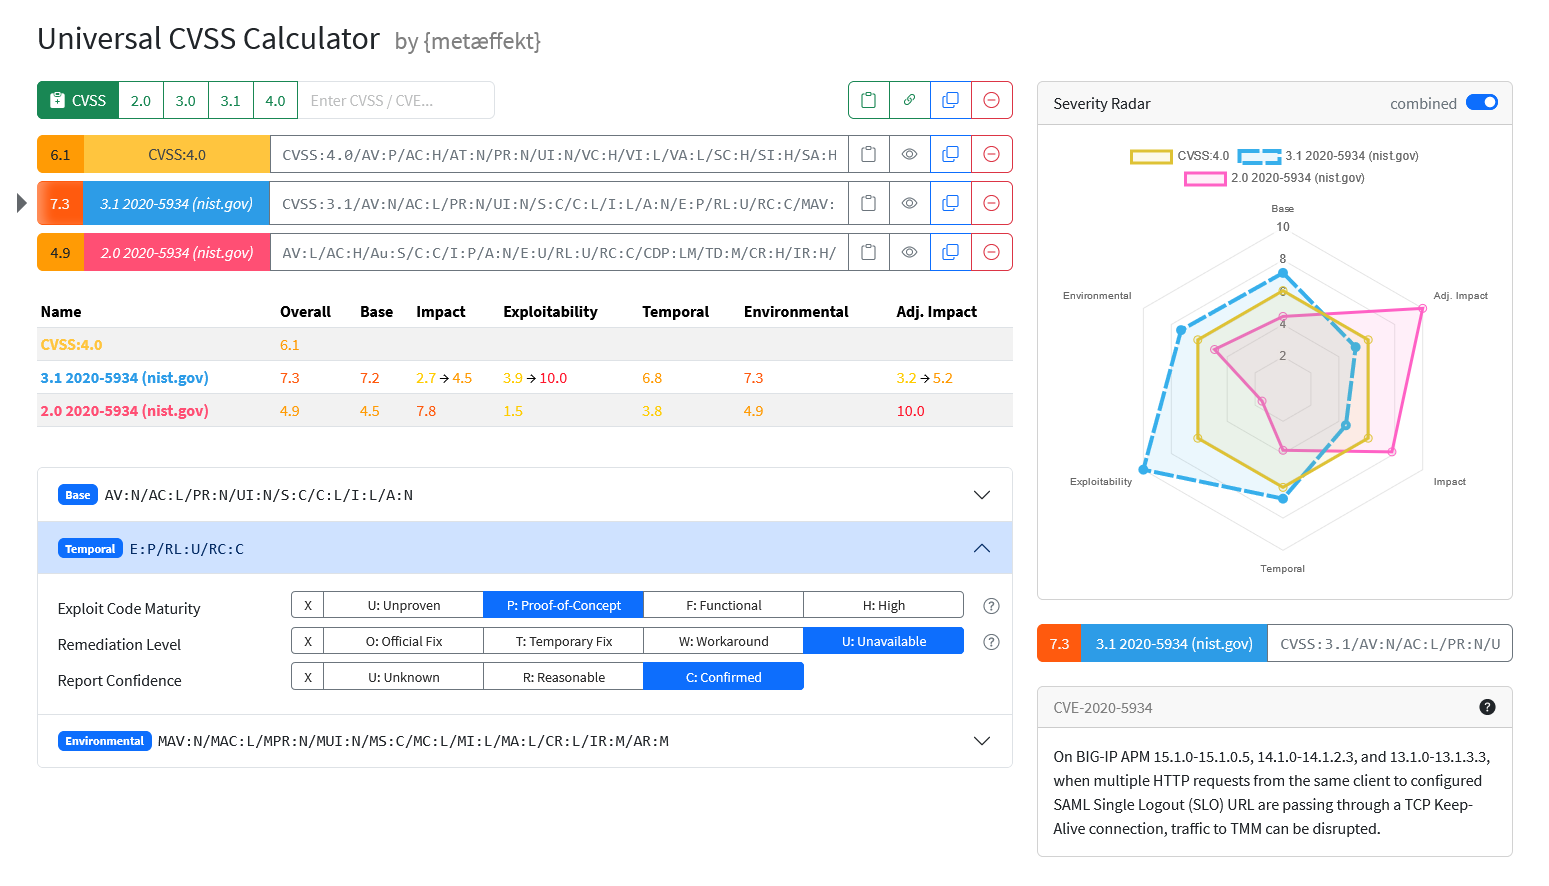
\includegraphics[width=0.8\textwidth, keepaspectratio]{res/img/metaeffekt-cvss-calculator-ui}
    \caption{Der {\metaeffekt} Universal CVSS-Rechner}
    \label{fig:metaeffekt-cvss-calculator-ui-initial}
\end{figure}

Von Herrn Shane Coughlan (OpenChain General Manager und ein Referent vom Open Source Forum der bitkom) haben wir freundlicherweise folgendes Zitat zu unserem Rechner erhalten:
\begin{quote}
    \textit{\qt{Contextualizing security threats is as important as identifying their existence,” says Shane Coughlan, OpenChain General Manager. “The emergence of open source tools to visualize this is a key part of ensuring the supply chain can plan ahead and action responses. We are delighted to see the work by Metaeffekt, an official OpenChain Partner, in the domain. It aligns well with OpenChain ISO/IEC 18974, the international standard for open source security assurance.}}
\end{quote}


%
\section{Woche 19 - Assessment-Policy \headerand Generation 3 Fertigstellung} \label{sec:bericht-wo-19-initial}

% 2024-01-22 bis 2024-01-26

\lweekdaymarginpar{\weekdayMondayShort\ - \weekdayWednesdayShort}

Einer der Kunden der \metaeffekt, den wir mit dem Schwachstell-Monitoring betreuen, geht nun in eine Projektphase, in der er Einschätzungen für Schwachstellen und Maßnahmen für deren Mitigierung vergeben möchte.
Dazu planen sie interne Workshops verpflichtend für mehrere Abteilungen anzubieten, wobei wir sie natürlich unterstützen wollen.

Darum schrieb ich die erste Hälfte der Woche an einer Assessment-Policy als Ausgangspunkt für ihre Überlegungen.
In diesem 6 Seiten langen Dokument berühre ich die folgenden Punkte:
Was ist der allgemeine Prozess, Vulnerability Monitoring durchzuführen?
Wie kann mit CVSS ein kontextualisiertes re-Scoring stattfinden?
Was sind die einzelnen CVSS Metriken der verschiedenen Versionen, die (Kontext-weit) verändert werden können/sollten?
Wie vergibt man einen Status, Risiken und Maßnahmen?
Wie werden Schwachstellen am besten priorisiert?

\sweekdaymarginpar{\weekdayThursdayLong}

Zusammen mit einer Kollegin habe ich dieses Dokument Donnerstag noch einmal überarbeitet und an meinen Chef übergeben, der es auch noch einmal überarbeitet und dann mit unseren Kunden durchgesprochen hat.

\sweekdaymarginpar{\weekdayFridayLong}

Passend dazu war Freitag dann der Tag, an dem der große Pull Request mit der Generation 3 unseres Vulnerability Monitorings ge-merged wurde.
Uns ist es besonders wichtig gewesen, die Änderungen aus dieser Version noch vor den Workshops des Kunden anzuwenden, denn so müssen nicht gleich einen Monat später neue Kurse für die neue Version angeboten werden.
Diese Änderungen zum Kunden zu bringen würde aber erst nächste Woche geschehen.

Den restlichen Tag habe ich noch einige Änderungen aufgrund von Feedback, das wir erhalten haben, an unserem CVSS-Rechner gemacht.
Freitag war außerdem ein alter Kollege zu Besuch, der vor einiger Zeit aufgehört hatte, hier zu arbeiten.


%
\section{Woche 20 - BSI-Meeting \headerand Integration von Generation 3} \label{sec:bericht-wo-20-initial}

% 2024-01-29 bis 2024-02-02

\lweekdaymarginpar{\weekdayMondayLong}

Montag war ein interessanter Tag, denn heute hatten wir ein Meeting mit Repräsentanten vom BSI bezüglich des CSAF-Standards und unseres CVSS-Rechners.
Beteiligt war vor allem Thomas Schmidt\footnote{\url{https://www.it-meets-industry.de/de/referent-thomas-schmidt}}, welcher bereits Leiter des CSAF-Workshops in München Ende letzten Jahres war, und Herr Von Samson.

Hierfür habe ich den Morgen eine Demo unseres Toolings vorbereitet, welche wir dann am Nachmittag zusammen mit vorbereiteten Fragen durchgesprochen haben.
Insgesamt war es ein sehr konstruktives Meeting, aus dem wir viele weitere Tasks ableiten konnten, vor allem zu Ansätzen zur Integration von CSAF in unseren Workflow.
Thomas Schmidt hat die folgenden Tage noch einige Issues auf unserem Repository des CVSS-Rechners auf GitHub erstellt, die ich Ende der Woche angehen würde.

\sweekdaymarginpar{\weekdayTuesdayShort\ - \weekdayThursdayShort}

Die restliche Woche habe ich mich mit der Integration von Generation 3 unseres Monitorings bei den Kunden beschäftigt.
Einer unserer Problempunkte war es bisher, dass teilweise Kunden noch auf Generation 1 standen, diese wollten wir nun alle zusammen einheitlich auf Generation 3 heben.
Insgesamt mussten drei Projekte fürs Erste ge-upgraded werden.

Dafür habe ich von meinem Chef nacheinander Zugriff auf je einen Kundenlaptop bekommen, bei denen je ein- oder mehrere Git-Projekte mit unserem Tooling, welche in deren Pipelines verwendet werden.
Der Prozess war immer der gleiche:
die vorhandenen Versionen und Konfigurationen mussten alle der Reihe nach aktualisiert werden, sodass sie dem neuen Format entsprechen.
Hier war der Migrationsguide, den ich zuvor (für genau diese Situation) verfasst hatte, viel wert.

Es gab natürlich unzählige Komplikationen und genauso viele Änderungen, die noch am Code gemacht werden mussten, die hier aufgelistet den Rahmen sprengen würden.
Mittwochs bin ich auch etwas länger geblieben, aber Donnerstagnachmittag waren alle Projekte aktualisiert und liefen durch.

\sweekdaymarginpar{\weekdayFridayLong}

Freitag bin ich die Issues\footnote{\url{https://github.com/org-metaeffekt/metaeffekt-universal-cvss-calculator/issues?q=is\%3Aissue+is\%3Aclosed}} von Thomas durchgegangen und habe die ersten davon bearbeitet.
Hier gab es nichts, das Probleme bereitet hätte (bis auf Issue \#2, hier hat sich das FIRST\footnote{\url{https://www.first.org/cvss}} bis Praktikumsende nicht zurückgemeldet).

Zudem gab es nach unserem Weekly ein Meeting mit dem Kunden, der die Assessment-Workshops plant bezüglich der Generation 3, der Änderungen und es bei ihnen final in ihre Pipeline zu integrieren.


%
\section{Woche 21 - Praktikumsbetreuung \headerand Abschluss des Praxissemesters} \label{sec:bericht-wo-21-initial}

% 2024-02-05 bis 2024-02-09

\lweekdaymarginpar{\weekdayMondayLong}

Die letzte Woche für mich im Praktikum bedeutete den Start eines anderen:
Die \metaeffekt\ hat einen BOGY-Praktikanten angenommen, der diese Woche einmal bei uns reinschnuppern durfte.
Ich war zu einem großen Teil für seine Betreuung verantwortlich, nebenbei habe ich noch weitere Probleme mit der Integration von Generation 3 bei den Kunden gelöst, die seit dem Ende der letzten Woche aufgetreten sind.

Mit dem Praktikanten habe ich erst einmal ein wenig programmieren und Konzepte in Java geübt, denn er sollte diese Woche hauptsächlich mit einem der Testing-Frameworks eines anderen Kollegen einige Testfälle für unseren Software-Scanner und Komponenten-Extraktor schreiben.

\sweekdaymarginpar{\weekdayTuesdayLong}

Er schien Konzepte recht schnell aufzunehmen und so konnte er bereits Dienstag mit den eigentlichen Testfällen beginnen.
Natürlich hat er ab und zu auch andere Probleme lösen und Dinge tun dürfen.

Ansonsten ist der Dienstag genau wie der Montag verlaufen - ich durfte wieder Probleme mit Generation 3 beheben.
Allerdings schien dieses Mal ein größeres Problem dabei zu sein:
Unser Prozess ist auf einmal von durchschnittlich 10 Minuten Laufzeit auf Generation 2 zu über zwei Stunden auf der dritten gesprungen.
Das ist natürlich nicht akzeptabel, und ich habe mich gleich an die Recherche gemacht.
Gewundert hat es mich allerdings schon, denn ich hatte bei meinen Tests bei dem neuen Datenmodell speed-ups von bis zu 200\% oder 300\% in optimalen Fällen gemessen.

Glücklicherweise konnte ich das Problem mit nur einer Zeile Code-Änderungen beheben:
Ich habe eine Liste zu einem Set umgewandelt, eine Übersehene nicht vollständig durchgeführte Optimierung meinerseits, die ich scheinbar vergessen hatte, fertig durchzuführen.
Dadurch sind wir bei nur noch zweieinhalb Minuten gelandet, was eher dem entsprach, was ich erwartet hatte.

\sweekdaymarginpar{\weekdayWednesdayShort, \weekdayThursdayShort}

Mittwoch und Donnerstag habe ich noch live in Kooperation mit einem Teams-Meeting die letzten Probleme beheben können, passend zum Ende meines Praktikums war also Generation 3 vollständig integriert.
Natürlich konnte ich auch noch mit dem Praktikanten einige Dinge tun und üben.

\sweekdaymarginpar{\weekdayFridayLong}

An meinem 100sten und damit letzten Tag des Praktikums habe ich zur Feier Kuchen mitgebracht und beim Weekly zusammen mit den restlichen süßen Stückchen verteilt.
Nach dem Weekly konnten wir auch noch alle zusammen aus dem Büro Currywurst essen gehen, es war also ein guter Abschluss zum Praktikum.

Natürlich wurde auch gearbeitet:
Ich habe den Tag dazu genutzt, einem weiteren Issue meines Chefs mit einem unserer Reports zu beheben.
Hier ging es um den periodischen Security-Advisory Report mit Bezug auf die Schwachstellsituation in einem Projekt.
Durch die neue Art zu filtern in Generation 3 hat er bemerkt, dass er nun gerne genauer kontrollieren können möchte, welche Daten in diesem Report angezeigt werden.
Hier habe ich also neue Parameter und alternative Report-Templates angelegt, die diesen Wünschen entsprechen.

Auch für den BOGY-Praktikanten war es der letzte Tag und so sind wir beide mit einem erfolgreich absolvierten Praktikum ins Wochenende gegangen.

Ich habe noch weitere 12 Tage bei dem Unternehmen mit meinen 35 Stunden in den folgenden Wochen gearbeitet und einen weiteren Vertrag für weitere Zusammenarbeit abgeschlossen.
Meine Reise in dieser Welt ist also noch lange nicht vorbei.


    \fi

    %! Author = Yan Wittmann


\chapter{Projektbericht} \label{ch:projektbericht}

In der Einleitung (Kapitel\ \ref{sec:projektbericht-projektziel}) wird zunächst auf die Abteilung im Unternehmen, die aktuelle Situation und die Ziele für das Projektsemester eingegangen.
Bei den darauf folgenden Grundlagen (Kapitel\ \ref{sec:projektbericht-grundlagen}) werden die relevanten Themen, Begriffe und Standards erklärt.

\section{Einleitung, Problemstellungen und Projektziel} \label{sec:projektbericht-projektziel}

Die für dieses Praktikum relevante Abteilung in der {\metaeffekt} stellt ein automatisiertes Vulnerability Monitoring her und integriert es bei diversen Kunden, deren Wünsche und Anforderungen priorisiert in die Systeme zurückgeführt werden.
Das Vulnerability Monitoring wird intern durch eine Aneinanderreihung von Prozessschritten modelliert, die auch als \qt{Inventory Enrichment Pipeline} bezeichnet wird.
Die Prozessschritte erhalten jeweils ein Software-Inventar als Eingabe, welches sie auf eine bestimmte definierte Weise modifizieren und für den nächsten Schritt bereitstellen, sodass ein Inventar, das alle Schritte durchlaufen hat, alle nötigen Schwachstell-Informationen angereichert bekommen hat.
Auf diese Pipeline wird im Kapitel\ \ref{subsec:projektbericht-grundlagen-vulnerability-monitoring} kurz eingegangen, sie soll allerdings nicht Hauptbestandteil dieses Berichts sein und dient nur zur besseren Einordnung der anderen Prozesse.

In dem Praktikum liegt der Schwerpunkt vor allem auf dem CVSS-Standard\textsuperscript{\ref{subsec:projektbericht-grundlagen-cvss}}, vor allem die Verbesserung unseres Supports für neuere Versionen dieses und konzeptionelle Änderungen, wie wir mit diesen umgehen wollen.
Konkret geht es um die folgenden Punkte:

\begin{smitemize}
    \item Die Veröffentlichung der neuesten Version 4.0 des CVSS-Standards am 31.\ Oktober 2023\footnote{\url{https://www.first.org/cvss/v4-0/}} wird über die nächsten Monate zur Folge haben, dass CVSS-Vektoren der Version 4.0 für Schwachstellen in den öffentlichen Datenbanken auftauchen werden, die wir in der Lage sein müssen, zu parsen und zu berechnen.
    Es ist dazu also notwendig, die aktuelle Implementierung der Versionen 2.0 und 3.1 um die vierte zu erweitern.
    Jedoch reicht hier nicht einfach die Implementierung der Berechnungslogik, um diesen Task abzuschließen, sie muss auch noch in die vorhandenen Systeme integriert und die Theorie dahinter verstanden werden, damit man gegenüber Kunden aussagekräftig die Unterschiede und die Vorteile begründen kann.
    \item Über die Monate vor dem Praktikum ist es bereits immer deutlicher geworden, dass das Datenmodell hinter dem Vulnerability Monitoring fast komplett neu geschrieben werden muss, um neue Anforderungen und Erkenntnisse effizient und korrekt unterstützen zu können.
    Die Anforderung an das Datenmodell, die hier relevant ist, ist eine bessere Art, die CVSS-Vektoren abzulegen und zu verarbeiten.
    Es wurde erkannt, dass meistens nicht nur ein CVSS-Vektor einer Quelle pro Schwachstelle (CVE, \ldots) vorhanden ist, sondern mehrere, die von mehreren Organisationen und Institutionen vergeben werden, da ihre Meinungen über den Schweregrad voneinander abweichen können.
    Bisher wird mit diesen zusätzlichen Vektoren nicht bewusst unterschiedlich umgegangen, es wird einfach der erste verarbeitet, der vorhanden ist.
    Um diese Situation zu verbessern, soll ein System eingeführt werden, das über die einzelnen Schritte der Inventory Enrichment Pipeline nur die Vektoren aggregiert und noch nicht verarbeitet oder berechnet.
    Erst zum Ende, wenn es darum geht die Reports (PDF, HTML) zu generieren, sollen die Vektoren ausgewählt, eventuell kombiniert und deren Scores berechnet werden.
    Bei dem Überarbeiten des Datenmodells muss also darauf geachtet werden, diese Anforderung zu unterstützen.
    Zudem muss ein CVSS-Selektor geschrieben werden, der die darzustellenden Vektoren berechnen kann.
    \item Zuletzt ging es noch um die Implementierung des CVSS-Standards in TypeScript, die Open Source gestellt werden sollte und mit einem Web-UI als online verfügbarer, interaktiver CVSS-Rechners verfügbar sein soll.
    Dieser soll dann aus den eigenen Reports verlinkt werden können.
    Der Grund hierfür ist simpel: Es gibt bisher keinen online CVSS-Rechner, der alle unsere Anforderungen erfüllt.
    Es gibt keinen Rechner, der alle Versionen zugleich unterstützt, keinen, der mehrere Vektoren gleichzeitig gut vergleichbar zulässt und leider haben viele der offiziellen Rechner auch Probleme, die URL-Parameter korrekt zu erkennen.
\end{smitemize}

In diesem Bericht wird ein Fokus auf die CVSS-seitigen Arbeiten gelegt, da sie den Großteil des Semesters eingenommen haben.

\section{Grundlagen} \label{sec:projektbericht-grundlagen}

\subsection{Software-Inventare} \label{subsec:projektbericht-grundlagen-inventories}

\subsection{NVD / NIST} \label{subsec:projektbericht-grundlagen-nvd-nist}

\subsection{CVE / CPE} \label{subsec:projektbericht-grundlagen-cve-cpe}

\subsection{CPE Derivation} \label{subsec:projektbericht-grundlagen-cpe-derivation}

\subsection{CVSS} \label{subsec:projektbericht-grundlagen-cvss}

\subsection{Vulnerability Assessment} \label{subsec:projektbericht-grundlagen-vulnerability-assessment}

\subsection{Automatisiertes Vulnerability Monitoring} \label{subsec:projektbericht-grundlagen-vulnerability-monitoring}

Die relevanten Prozessschritte sind das automatische Zuordnen von CPEs zu den Produkten aus den Kundeninventaren (CPE Derivation\textsuperscript{\ref{subsec:projektbericht-grundlagen-cpe-derivation}})


    %! Author = Yan Wittmann

\chapter{Ergebnisse} \label{ch:ergebnisse}

In dem Praxissemester wurden unter anderem die folgenden Haupt-Ergebnisse erzielt:

\begin{itemize}
    \item Implementierung des CVSS 4.0 Standards in die vorhandene Softwarelösung und Integration in den Daten-Mirror und die Reporting-Tools.
    \item Überarbeitung des Datenmodells zur Unterstützung von mehreren CVSS-Vektoren je Schwachstelle, verbessertem Tracking der Quellen von Schwachstellen und der Generalisierung der Datenzugriffe um Redundanzen in den Implementierungen zu vermeiden.
    \item Implementierung der CVSS-Versionen 2.0, 3.0, 3.1 und 4.0 in TypeScript.
    \item Entwickeln eines online-CVSS-Rechners, der aus den eigenen Reporting-Tools referenziert wird und bereits bei verschiedenen Events vorgestellt wurde.
    \item Integration der durchgeführten Änderungen in die entsprechenden Kundenprojekte an den Kundensystemen und im konstanten Dialog mit den Zuständigen.
    \item Besuchen des Arbeitskreises OpenSource des {\bitkom} und halten eines Vortrages vor anderen Firmen.
    \item Besuchen des Open Source Forums des {\bitkom} in Erfurt.
    \item Besuchen des zweitägigen CSAF-Workshops in München im ISH (Information Security Hub), durchgeführt vom BSI\@.
\end{itemize}

Die folgenden konkreten öffentliche Ergebnisartefakte wurden dabei unter anderem erzeugt (mit Links hinterlegt):

\begin{itemize}[noitemsep]
    \item \href{https://www.metaeffekt.com/security/cvss/calculator}{Universal CVSS Calculator}
    \item \href{https://github.com/org-metaeffekt/metaeffekt-universal-cvss-calculator}{GitHub Repository der TypeScript Implementierung}
    \item \href{https://youtu.be/R2S0_6-NQGQ?si=d7zpxbJ7P4R26nRb&t=2801}{Webinar zum CVSS Calculator}
    \item \href{https://mvnrepository.com/artifact/com.metaeffekt.artifact.analysis/ae-artifact-analysis}{Weiterführung des aritfact-analysis Projektes}
    \item \href{https://github.com/org-metaeffekt/metaeffekt-core}{Weiterführung des Core Projektes}
\end{itemize}


    %! Author = Yan Wittmann

\chapter{Ausblick} \label{ch:ausblick}

Meine Mitarbeit bei der {\metaeffekt} wird nach dem Praxissemester weiterhin fortgeführt.
In diesem Zusammenhang werde ich mit den Systemen, Kunden und Kollegen auch weiterhin in Kontakt bleiben und die Entwicklungen begleiten.

Konkret werden in der nächsten Zeit die folgenden Punkte relevant:

\begin{itemize}
    \item Integration von KEV (Known Exploited Vulnerabilities) in die bestehenden Systeme.
    \item Integration von CSAF (Common Security Advisory Framework) als Advisory-Quelle und Support für Export von CSAF-Dateien aus gescannten Software-Inventaren.
    \item Besuch des KIT, um mit einem Professor über das Thema Vulnerability Chaining zu sprechen, welches in nächster Zeit bei uns mit einem eigenen Konzept integriert werden soll.
    \item Neuschreiben des VAD (Vulnerability Assessment Dashboards) mit TypeScript.
    \item Erstellen eines \qt{Overview Reports} in HTML und TypeScript, für eine Übersicht über mehrere Kontexte.
    \item Um unsere Systeme mehr eine Art Tooling-Chain bauen, um den Einstieg in die Verwendung unserer Tools zu erleichtern.
    \item Präsentieren unseres Toolings auf der großen Bühne beim Open Source Forum des {\bitkom} in Erfurt im September.
    \item Erstellung eines Test-Frameworks für das Vulnerability Monitoring.
\end{itemize}


    \newpage

% Listen wenn überhaupt ans Ende und nicht an den Anfang.
% Meist ist das aber unnötig.
    \listoffigures % Liste der Abbildungen
%\begingroup % aahh nicht noch ein pagebreak
%\let\clearpage\relax %
    % \listoftables % Liste der Tabellen
%\endgroup

% Glossar kommt auch ans Ende
%\glsaddall % das fügt alle Glossar-Einträge ein
%\printglossaries % nicht vergessen "makeglossaries praksem" aufzurufen
%\gls{Computer}
%\newpage

    \addcontentsline{toc}{chapter}{Literaturverzeichnis}
    %\bibliographystyle{plain}
    %\bibliography{praksem}
    \printbibliography
% \bibliography{praksem,online} # wenn man zwei Dateien hätte

% Das wäre die Alternative mit geteilten Quellen (preamble muss auch
% angepasst werden) und die Literatur muss in die Datei praksem.bib
% und die Online-Quellen müssen in die Datei online.bib.
%\begin{btSect}{praksem} % mit bibtopic Quellen trennen
%\section*{Literaturverzeichnis}
%\addcontentsline{toc}{chapter}{Literaturverzeichnis}
%\btPrintCited
%\end{btSect}
%\begin{btSect}{online}
%\section*{Online-Quellen}
%\addcontentsline{toc}{chapter}{Online-Quellen}
%\btPrintCited
%\end{btSect}
% dann ab und zu "bibtex praksem1" und "bibtex praksem2" aufrufen

\end{document}
;;; Local Variables:
;;; ispell-local-dictionary: "de_DE-neu"
;;; End:
